\documentclass[a4paper, 12pt]{report}

\usepackage[dvipsnames]{xcolor}

%%%%%%%%%%%%%%%%
% Set Variables %
%%%%%%%%%%%%%%%%

\def\useItalian{1}  % 1 = Italian, 0 = English

\def\courseName{Calcolo delle Probabilità}

\def\coursePrerequisites{Apprendimento del materiale relativo al corso \textit{Metodi Matematici per l'Informatica}}

\def\book{\curlyquotes{The Probability Tutoring Book}, C. Ash}

\def\authorName{Simone Bianco}
\def\email{bianco.simone@outlook.it}
\def\github{https://github.com/Exyss/university-notes}
\def\linkedin{https://www.linkedin.com/in/simone-bianco}


%%%%%%%%%%%%
% Packages %
%%%%%%%%%%%%

\usepackage{../../../packages/Nyx/nyx-packages}
\usepackage{../../../packages/Nyx/nyx-styles}
\usepackage{../../../packages/Nyx/nyx-frames}
\usepackage{../../../packages/Nyx/nyx-macros}
\usepackage{../../../packages/Nyx/nyx-title}
\usepackage{../../../packages/Nyx/nyx-intro}

%%%%%%%%%%%%%%
% Title-page %
%%%%%%%%%%%%%%

\logo{../../../packages/Nyx/logo.png}

\if\useItalian1
    \institute{\curlyquotes{\hspace{0.25mm}Sapienza} Università di Roma}
    \faculty{Ingegneria dell'Informazione,\\Informatica e Statistica}
    \department{Dipartimento di Informatica}
    \ifdefined\book
        \subtitle{Appunti integrati con il libro \book}
    \fi
    \author{\textit{Autore}\\\authorName}
\else
    \institute{\curlyquotes{\hspace{0.25mm}Sapienza} University of Rome}
    \faculty{Faculty of Information Engineering,\\Informatics and Statistics}
    \department{Department of Computer Science}
    \ifdefined\book
        \subtitle{Lecture notes integrated with the book \book}
    \fi
    \author{\textit{Author}\\\authorName}
\fi


\title{\courseName}
\date{\today}

% \supervisor{Linus \textsc{Torvalds}}
% \context{Well, I was bored\ldots}

%%%%%%%%%%%%
% Document %
%%%%%%%%%%%%

\begin{document}
    \maketitle

    % The following style changes are valid only inside this scope 
    {
        \hypersetup{allcolors=black}
        \fancypagestyle{plain}{%
        \fancyhead{}        % clear all header fields
        \fancyfoot{}        % clear all header fields
        \fancyfoot[C]{\thepage}
        \renewcommand{\headrulewidth}{0pt}
        \renewcommand{\footrulewidth}{0pt}}

        \romantableofcontents
    }

    \introduction

    \chapter{Introduzione alla probabilità}

    \section{Probabilità classica e limitazioni}

    Prima di poter parlare di probabilità, è necessario definire ciò di cui essa si occupa. Il calcolo di una probabilità corrisponde allo studio di un fenomeno osservabile esclusivamente dal punto di vista della possibilità o meno del suo verificarsi. La probabilià è uno strumento molto utile per effettuare ragionamenti e prendere decisioni, ma essa può essere \textit{interpretata} in svariati modi.

    Supponiamo ad esempio di trovarci in ospedale. Il nostro amico Marco è molto malato ed ogni trattamento sembra fallire. Un dottore ci notifica dell'esistenza di un farmaco che possa \textit{probabilmente} salvargli la vita. Preoccupati, chiediamo al dottore quale sia la probabilità che il farmaco funzioni. Il medico afferma, tramite le sue conoscenze del campo, che \curlyquotes{con buona probabilità} il farmaco funzionerà. Volendo utilizzare un approccio più matematico, chiediamo il rateo di successo del farmaco su 100 pazienti, ossia quanti dei 100 pazienti sono guariti dopo la somministrazione. Dopo aver controllato, il medico afferma che il rateo sia 65 casi su 100, rassicurandoci.

    L'affermazione iniziale del medico si basa su una probabilità data dal \textbf{pensiero soggettivo}, mentre la nostra domanda finale si basa su una probabilità data dalla \textbf{frequenza degli esiti}. Di primo occhio, penseremmo che il nostro approccio sia \curlyquotes{più matematico} o \curlyquotes{più corretto}. Uno scettico potrebbe però contestare anche la nostra affermazione:
    \begin{itemize}
        \item E se le condizioni iniziali degli esiti presi in analisi sono diverse?
        \item E se il farmaco viene somministrato per la prima volta dal medico?
        \item E se gli esiti registrati sono stati tutti fortuiti?
        \item E se aumentando il campione il rateo di successo diminuisce?
    \end{itemize}

    Con solo questo caso in analisi, concludiamo facilmente che parlare di probabilità è \textit{molto} difficile. L'obiettivo principale di questo capitolo è quindi quello di introdurre concetti elementari che ci permettano di discutere di probabilità. In particolare, ci concentreremo inizialmente sulla \textbf{probabilità classica}. Questa tipologia elementare di probabilità si basa sul concetto di \textbf{eventi} ed \textbf{esiti}.
    
    Consideriamo ad esempio il lancio di una moneta. Tale \textit{evento} può avere solo due \textit{esiti}: testa o croce. Intuitivamente, ci aspettiamo che ciascuno dei due esiti abbia il 50\% di probabilità di accadere, ossia \curlyquotes{metà e metà}. Nella probabilità classica, questi due esiti costituiscono lo \textbf{spazio ambiente}, vale a dire l'insieme di tutti gli esiti possibili per il fenomeno preso in esame. Lo spazio ambiente viene generalmente indicato con il simbolo $\Omega$, mentre gli esiti vengono generalmente indicati con un numero. Ad esempio, in questo caso abbiamo $\Omega = \{0,1\}$, dove l'esito 0 corrisponde a \curlyquotes{croce} e l'esito 1 corrisponde a \curlyquotes{testa}.

    Nella probabilità classica, la probabilità di un evento $A$ viene (solitamente) calcolata utilizzando la frequenza degli esiti positivi nello spazio ambiente, ossia la quantità di esiti dello spazio ambiente che rende vero l'evento $A$. In questo caso, dunque, abbiamo che:
    \[\Pr[\text{il risultato del lancio è testa}] = \frac{\text{numero di esiti testa}}{\text{numero di esiti totali}}\]

    Questa tipologia di probabilità può essere comodamente modellata tramite la teoria degli insiemi. In particolare, dato lo spazio ambiente $\Omega$, possiamo definire un \textbf{evento} come un semplice sottoinsieme di $A \subseteq \Omega$, dove gli elementi di $A$ corrispondono a tutti gli esiti che rendono vero l'evento $A$. Ad esempio, l'insieme $T = \{1\}$ corrisponde all'evento \curlyquotes{testa}. Questo ci permette di calcolare la probabilità dell'esempio precedente nel seguente modo:
    \[\Pr[T] = \frac{\abs{T}}{\abs{\Omega}} = \frac{1}{2} = 50\%\]

    ottenendo il 50\% di probabilità che ci aspettavamo. Tuttavia, notiamo facilmente che questa interpretazione della probabilità non è sempre un corretto modello:
    \begin{itemize}
        \item E se la moneta è stata truccata al fine di rendere uno dei due esiti più probabile?
        \item E se lo spazio ambiente contiene un numero infinito di esiti?
    \end{itemize}

    Per la prima domanda, il modello può essere \curlyquotes{spremuto} in modo da forzare un modello corretto. Ad esempio, se la moneta è stata truccata in modo da ottenere il 75\% delle volte l'esito \curlyquotes{testa}, possiamo considerare lo spazio ambiente $\Omega' = \{0,1,11,111\}$ ed imporre che $T' = \{1,11,111\}$ e che $C' = \{0\}$, dove $C$ è l'evento descrivente l'esito \curlyquotes{croce}. In questo modo, otteniamo che:
    \[\Pr[T'] = \frac{\abs{T'}}{\abs{\Omega'}} = \frac{3}{4} = 75\%\]

    Per il secondo caso, invece, è chiaramente impossibile adattare il modello in quanto non possiamo dividere per una cardinalità infinita. Vedremo nelle sezioni successive un modello \textbf{assiomatico} della probabilità che ci permetterà di risolvere entrambe le problematiche (e molte altre) comodamente.

    \begin{frameddefn}{Spazio ambiente ed Evento (prob. classica)}
        Dato un insieme finito $\Omega = \{\omega_1, \ldots, \omega_n\}$ detto spazio ambiente, definiamo un sottoinsieme $A \subseteq \Omega$ come evento su $\Omega$. 
        La probabilità classica dell'evento $A$ è definita come:
        \[\Pr[A] = \frac{\abs{A}}{\abs{\Omega}}\]

        \textit{Nota}: il simbolo $\omega$ corrisponde all'Omega greco minuscolo, non alla lettera $w$
    \end{frameddefn}

    \section{Modelli principali del Calcolo Combinatorio}

    Dopo aver enunciato le basi della probabilità classica, risulta evidente la necessità di ripassare le basi del \textbf{calcolo combinatorio}, ossia la branca della matematica atta a studiare metodi per computare quantità di elementi ed oggetti. Difatti, domande come \curlyquotes{qual è la probabilità di pescare un asso da un mazzo di 52 carte francesi?} nella probabilità classica vengono ridotte a due sotto-problemi: calcolare la quantità di assi in un mazzo di 52 carte francesi (vale a dire 4, 1 per seme) e la quantità di carte in un mazzo di 52 carte francesi (vale a dire 52, ovviamente).

    In questa sezione verranno riassunte le basi del calcolo combinatorio, elencandone i principali principi e modelli. \underline{Per appunti più approfonditi sull'argomento} (in particolare spiegazioni ed esempi ulteriori delle formule mostrate in seguito), si rimanda agli appunti del corso \textit{Metodi Matematici per l'Informatica} (\href{https://github.com/Exyss/university-notes}{reperibili qui}).
    
    Partiamo con un problema semplice. Supponiamo che in un urna vi siano 3 palline bianche e 2 palline nere. Ci chiediamo quale sia la probabilità che,
    estraendo due palline, la seconda sia bianca? Formalizziamo il problema secondo il modello della probabilità classica. Prima di tutto, individuiamo l'\textbf{evento elementare}, ossia la forma assunta da un singolo esito, come l'estrazione \textit{ordinata} di due palline $\omega=(\omega_1,\omega_2)$, dove $\omega_1$ è la prima pallina estratta e $\omega_2$ è la seconda pallina estratta.
    
    Possiamo numerare le palline da 1 a 5, dicendo che le palline bianche son quelle da 1 a 3, mentre le restanti sono nere. Detto ciò, possiamo capire che l'insieme degli eventi elementari, cioè lo spazio ambiente, corrisponde a tutte le coppie di numeri naturali compresi fra 1 a 5 senza ripetizioni.
    \[\Omega = \{(\omega_1,\omega_2) \mid \omega_1 \in \{1,2,3,4,5\}, \omega_2 \in \{1,2,3,4,5\} - \{\omega_1\}\}\]

    È di facile intuizione capire che $\abs{\Omega}=5 \cdot 4 = 20$ poiché abbiamo 5 possibilità per la prima pallina e 4 possibilità per la seconda pallina (visto che una è stata già pescata), dunque è sufficiente moltiplicare le varie combinazioni tra loro. In questo caso, abbiamo implitamente utilizzato il \textbf{principio moltiplicativo}, il quale afferma che dati due insiemi finiti $A,B$ si ha che:
    \[\abs{A \times B} = \abs{A} \cdot \abs{B}\]

    Tornando all'esempio, definiamo come $B_2$ l'evento \curlyquotes{la seconda pallina estratta senza ripetizioni è bianca}. Formalmente, abbiamo che:
    \[B_2 = \{(\omega_1,\omega_2) \in \Omega \mid \omega_2 \in \{1,2,3\}\}\]
    
    Ancora una volta, tramite il principio moltiplicativo osserviamo facilmente che $\abs{B_2} = 4 \cdot 3 = 12$ poiché per la seconda estrazione abbiamo 3 possibili palline bianche e per la prima estrazione abbiamo tutte le altre rimanenti (non ci interessa il colore essendo la prima estrazione). Possiamo quindi concludere che:
    \[\Pr[B_2] = \frac{\abs{B_2}}{\abs{\Omega}} = \frac{12}{20} = \frac{3}{5} = 0.6\]
    
    Passiamo adesso al riepilogo di alcuni modelli fondamentali nella quale spesso ricadono i problemi di conteggio. L'idea principale dietro ogni modello viene comunemente metaforizzata secondo il problema delle palline nelle urne.
    \begin{itemize}
        \item \textbf{Disposizioni senza ripetizione di classe $k$ per $n$ elementi}. Si hanno $n$ palline numerate dentro un urna e si vogliono fare \(k\) estrazioni con \textit{senza rimpiazzo} (ossia ogni pallina pescata viene eliminata dall'urna). L'ordine di estrazione delle palline è di nostro interesse, sequenze come $1,2,3$ e $1,3,2$ vengono considerate come \textit{diverse}. Per problemi di questo tipo, la quantità $D_{n,k}$ di sequenze possibili estraendo $k$ palline su $n$ totali è data da:
        \[D_{n,k} = \frac{n!}{(n-k)!}\]
        Quando $k =n$, questo modello viene detto \textbf{permutazione}.
        \item \textbf{Disposizioni con ripetizione di classe $k$ per $n$ elementi}. Si hanno $n$ palline numerate dentro un urna e si vogliono fare \(k\) estrazioni \textit{con rimpiazzo} (ossia ogni pallina pescata viene subito reinserita nell'urna). L'ordine di estrazione delle palline è di nostro interesse, dunque sequenze come $1,2,3$ e $1,3,2$ vengono considerate come \textit{diverse}. Per problemi di questo tipo, la quantità $D'_{n,k}$ di sequenze possibili estraendo $k$ palline su $n$ totali è data da:
        \[D'_{n,k} = n^k\]
        \item \textbf{Combinazioni di classe $k$ per $n$ elementi}. Si hanno $n$ palline numerate dentro un urna e si vogliono fare \(k\) estrazioni \textit{senza rimpiazzo} (ossia ogni pallina pescata viene subito reinserita nell'urna). L'ordine di estrazione delle palline è di nostro interesse, dunque sequenze come $1,2,3$ e $1,3,2$ vengono considerate come \textit{uguali}. Per problemi di questo tipo, la quantità $C_{n,k}$ di sequenze possibili estraendo $k$ palline su $n$ totali è data da:
        \[C_{n,k} = \frac{n!}{k! (n-k)!} = \binom{n}{k}\]
        dove $\binom{n}{k}$ è il \textbf{coefficiente binomiale}
        \item \textbf{Anagrammi di classi $k_1, \ldots, k_m$ per $n$ elementi}. Si hanno $n$ palline numerate dentro un urna. Le palline sono di $m$ tipologie e per ogni tipologia $i$ vi sono $k_i$ palline (dunque $k_1 + \ldots + k_m = n$). Si vogliono fare $n$ estrazioni \textit{senza rimpiazzo} (ossia ogni pallina pescata viene subito reinserita nell'urna). L'ordine di estrazione delle palline è di nostro interesse, ma le palline della stessa tipologia vengono considerate come uguali tra loro, dunque sequenze come $1_R, 2_R, 3_B$ e $2_R, 3_B, 1_R$ (dove $R$ e $B$ rappresentano la tipologia della pallina) vengono considerate \textit{uguali} mentre sequenze come $1_R, 2_R, 3_R$ e $1_R, 2_R, 3_B$ vengono considerate \textit{diverse}. Per problemi di questo tipo, la quantità $A_{k_1, \ldots, k_m}$ di sequenze possibili estraendo $n$ palline su $n$ totali è data da:
        \[A_{k_1, \ldots, k_m} = \frac{n!}{k_1! \cdot \ldots \cdot k_m !} = \binom{n}{k_1, \ldots, k_m}\]
        dove $\binom{n}{k_1, \ldots, k_m}$ è il \textbf{coefficiente multinomiale} 
    \end{itemize}

    È opportuno osservare come il coefficiente binomiale sia un caso speciale del coefficiente multinomiale dove vi sono solo due tipologie: quella contenente gli oggetti di nostro interesse e quella che non li contiene. 
    Ricordiamo inoltre l'identità conosciuta come \textbf{binomio di Newton}, la quale afferma che:
    \[(a+b)^n = \sum_{k = 0}^n \binom{n}{k} a^k b^{n-k}\]
    
    Vediamo ora alcuni esempi per comprendere come applicare tali modelli combinatori nel calcolo delle probabilitè classiche.
    \begin{enumerate}
        \item Un codice PIN è formato da 4 cifre scelte tra 0 e 9 (quindi 10 cifre totali). Le cifre possono ripetersi (es. 1123 è valido) e l'ordine di digitazione conta (dunque 1234 è diverso da 4321). Supponiamo che un ladro voglia indovinare il PIN di un bancomat inserendo un codice casuale. Vogliamo sapere quale sia la probabilità dell'evento $A$ definito come \curlyquotes{il ladro indovina il PIN al primo tentativo}.
        
        Osserviamo come la quantità di esiti totali, ossia la cardinalità dello spazio ambiente, sia data da tutti i PIN possibili, i quali sono modellati da una disposizione con ripetizione di classe $4$ per $10$ elementi. Concludiamo quindi che $\abs{\Omega} = D'_{10,4} = 10^4$. Inoltre, è evidente che esista un solo esito favorevole all'evento $A$, vale a dire il PIN da indovinare. Concludiamo quindi che:
        \[\Pr[A] = \frac{1}{10^4} = 0.01\%\] 

        \item In una classe di 20 studenti, si devono eleggere una delegazione di 3 rappresentanti con ruoli distinti: presidente, vicepresidente e segretario. Ogni studente può essere eletto per un solo ruolo e  (ad esempio vi è distinzione tra il caso in cui Marco viene eletto come presidente e il caso in cui viene eletto come vicepresidente). Vogliamo sapere quale sia la probabilità dell'evento $B$ definito come \curlyquotes{Anna, Marco e Luca vengono eletti in questo ordine}.
        
        Osserviamo come la quantità di esiti totali sia data da tutte delegazioni da 3 rappresentanti possibili, le quali sono modellati da una disposizione senza ripetizione di classe $3$ per $20$ elementi. Concludiamo quindi che $\abs{\Omega} = \frac{20!}{17!} = 20 \cdot 19 \cdot 18$. Inoltre, è evidente che esista un solo esito favorevole all'evento $B$, ossia la delegazione Anna, Marco e Luca. Concludiamo quindi che:
        \[\Pr[B] = \frac{1}{\frac{20!}{17!}} = \frac{1}{20 \cdot 19 \cdot 18} = \frac{1}{6840} \approx 0.0001\%\] 


        \item Considerando la stessa situazione del punto precedente, vogliamo ora sapere la probabilità dell'evento $C$ definito come \curlyquotes{Anna, Marco e Luca vengono eletti in qualsiasi ordine}.
        
        La cardinalità dello spazio ambiente rimane chiaramente inalterata, ma la quantità di esiti favorevoli aumenta. In particolare, tali esiti sono modellati da una dispozione senza ripetizione di classe $3$ per $3$ elementi (ossia una permutazione di $3$ elementi), dunque $\abs{C} = \frac{3!}{0!} = 3 \cdot 2 \cdot 1$. Concludiamo quindi che: 
        \[\Pr[C] = \frac{\frac{3!}{0!}}{\frac{20!}{17!}} = \frac{3 \cdot 2 \cdot 1}{20 \cdot 19 \cdot 18} = \frac{1}{1140} \approx 0.0009\%\]

        \item Da un mazzo standard di 52 carte francesi, si estraggono 5 carte casualmente, senza rimetterle nel mazzo (come nel poker classico). Vogliamo sapere la probabilità dell'evento $D$ definito come \curlyquotes{la mano pescata è composta da esattamente una carta cuori}.
        
        Osserviamo come la quantità di esiti totali sia data da tutte pescate di 5 carte possibili, le quali sono modellati da una combinazione di classe $5$ per $52$ elementi, dunque $\abs{\Omega} = \binom{52}{5}$. Per quanto riguarda la quantità di esiti favorevoli, anche essi  possono essere modellati dalle combinazioni. In particolare, poiché l'ordine di pescata non conta, gli eventi favorevoli sono modellati dalle pescate in cui viene pescata 1 carta dalle 13 di cuori disponibili e 4 carte dalle 39 rimanenti, senza contare l'ordine di pescata, dunque $\abs{D} = \binom{13}{1} \binom{39}{4}$. Concludiamo quindi che: 
        \[\Pr[D] = \frac{\binom{13}{1} \binom{39}{4}}{\binom{52}{5}} = \frac{1069263}{2598960} \approx 0.41\%\]
    \end{enumerate}

    \section{Operazioni tra eventi}

    La definizione data di probabilità classica ci permette di prendere in prestito alcuni concetti della teoria degli insiemi ed applicarli nel calcolo delle probabilità. Ad esempio, consideriamo il lancio di un dado (non truccato) a 6 facce,  descritto dallo spazio ambiente $\Omega = \{1,2,3,4,5,6\}$. Consideriamo ora l'evento $P$ descritto dagli esiti in cui la faccia risultante sia un numero pari, ossia $P = \{2,4,6\}$. Sia inoltre $F_{\leq 3}$ l'evento descritto dagli esiti in cui la faccia risultate sia un numero minore o uguale a 3, ossia $F_{\leq 3} = \{1,2,3\}$.

    Consideriamo quindi l'evento \curlyquotes{la faccia risultante è un numero pari ed è un numero minore o uguale a 3}. Tramite la teoria degli insiemi, questo evento è facilmente descrivibile tramite l'\textbf{intersezione} $P \cap F_{\leq 3} = \{2\}$, ottenendo quindi che:
    \[\Pr[P \cap F_{\leq 3}] = \frac{\abs{P \cap F_{\leq 3}}}{\abs{\Omega}} = \frac{1}{6}\]

    Similmente, l'evento \curlyquotes{la faccia risultante è un numero pari o è un numero minore o uguale a 3} è describile come l'\textbf{unione} $P \cup F_{\leq 3} = \{1,2,3,4,6\}$, ottenendo quindi che:
    \[\Pr[P \cup F_{\leq 3}] = \frac{\abs{P \cup F_{\leq 3}}}{\abs{\Omega}} = \frac{5}{6}\]


    Altre basilari operazioni insiemistiche sono la \textbf{differenza} e il \textbf{complemento}. Dati due insiemi $A, B \subseteq \Omega$, la differenza insiemistica di $A$ con $B$ corrisponde all'insieme $A-B$ definito come:
    \[A-B = \{x \in A \mid x \notin B\}\]
    ossia l'insieme degli elementi di $A$ che non si trovano in $B$. Osserviamo come tale operazione sia \textit{non commutativa}. Ad esempio, per gli eventi precedenti abbiamo che $P - F_{\leq 3} = \{4,6\}$ e che $F_{\leq 3} - P = \{1,3\}$.

    Il complemento insiemistico su un insieme $A \subseteq \Omega$, indicato con $\overline{A}$ (oppure $A^c$), corrisponde al sottoinsieme dello spazio ambiente contenente tutti gli esiti opposti che non rientrano nell'evento $A$, vale a dire:
    \[\overline{A} = \{x \in \Omega \mid x \notin A\}\]

    In altre parole, abbiamo che $\overline{A} = \Omega -A$. Osserviamo come tale operazione sia un'\textit{involuzione}, vale a dire un'operazione inversa di se stessa. Difatti, abbiamo che:
    \[\overline{\overline{A}} = \Omega - (\Omega - A) = \{x \in \Omega \mid x \notin \Omega - A\} = \{x \in \Omega \mid x \in A\} = A\]

    In questi casi, risultano fondamentali le principali proprietà insiemistiche di base di seguito elencate (con le quali si dovrebbe già essere familiari):
    \begin{itemize}
        \item \textit{Proprietà disgiuntiva}:
        \[A \cap \overline{A} = \varnothing\]
        \item \textit{Proprietà associativa}: 
        \[A \cup (B \cup C) = (A \cup B) \cup C \qquad A \cap (B \cap C) = (A \cap B) \cap C\]
        \item \textit{Proprietà distributiva}: 
        \[A \cap (B \cup C) = (A \cap B) \cup (A \cap C) \qquad A \cup (B \cap C) = (A \cup B) \cap (A \cup C)\]
        \item \textit{Leggi di De Morgan}:
        \[\overline{A \cup B} = \overline{A} \cap \overline{B} \qquad \overline{A \cap B} = \overline{A} \cup \overline{B}\]
        \item \textit{Principio di inclusione-esclusione}:
        \[\abs{A \cup B} = \abs{A} + \abs{B} - \abs{A \cap B}\]
    \end{itemize}

    L'uso di questi operatori insiemistici risulta fondamentale nella probabilità classica, poiché esso ci permette di \curlyquotes{riscrivere} molti eventi complessi in termini di eventi meno complicati. Di seguito, riportiamo due esempi:
    \begin{enumerate}
            \item Consideriamo ancora l'evento $P \cap F_{\leq 3}$ descritto precedentemente. Consideriamo ora gli eventi $F_{= 3}$ e $F_{< 3}$, definiti analogamente. Osserviamo facilmente che $F_{\leq 3} = F_{= 3} \cup F_{< 3}$. Per tanto, abbiamo che:
            \[P \cap F_{\leq 3} = P \cap (F_{= 3} \cup F_{< 3}) = (P \cap F_{= 3}) \cup (P \cap F_{< 3}) = \varnothing \cup \{2\} = \{2\}\]

            concludendo quindi che:
            \[\Pr \sbk{P \cap F_{\leq 3}} = \frac{\abs{P \cap F_{\leq 3}}}{\abs{\Omega}} = \frac{1}{6}\]

            \item Tramite le \textit{leggi di De Morgan} possiamo riscrivere l'evento \curlyquotes{la faccia risultate non è né un numero pari né un numero minore o uguale a 3}, ossia l'evento $\overline{P} \cap \overline{F_{\leq 3}}$ come l'evento \curlyquotes{la faccia risultante non è un numero pari o un numero minore o uguale a 3}, ossia l'evento $\overline{P \cup F_{\leq 3}}$, concludendo che:
            \[\Pr \sbk{\overline{P} \cap \overline{F_{\leq 3}}} = \Pr \sbk{\overline{P \cup F_{\leq 3}}} = \frac{\abs{\overline{P \cup F_{\leq 3}}}}{\abs{\Omega}} = \frac{1}{6}\]
            dove $\overline{P \cup F_{\leq 3}} = \{5\}$.
    \end{enumerate}

    Osserviamo inoltre come gli eventi complementari ci permettano di derivare una prima fondamentale proprietà della probabilità classica (che verrà estesa anche agli altri tipi di probabilità). Dato un evento $A \subseteq \Omega$, poiché $\Omega$ contiene tutti gli elementi di $A$ abbiamo che:
    \[\Pr\sbk{\overline{A}} = \frac{\abs{\Omega - A}}{\abs{\Omega}} = \frac{\abs{\Omega} -\abs{A}}{\abs{\Omega}} = 1 - \frac{\abs{A}}{\abs{\Omega}} = 1 - \Pr[A]\]

    In altre parole, la probabilità di un evento complementare è uguale a 1 meno la probabilità dell'evento di partenza.

    \begin{framedthm}{Probabilità di un evento complementare}
        Dato un evento $A \subseteq \Omega$, si ha che:
        \[\Pr\sbk{\,\overline{A}\,} = 1- \Pr[A]\]
    \end{framedthm}

    Similmente, il \textit{principio di inclusione-esclusione} nella probabilità classica ci permette di riscrivere la probabilità di eventi disgiunti (cioè quelli della forma \curlyquotes{A o B}) tramite somme e differenze. Dati due eventi $A, B  \subseteq \Omega$, abbiamo che:
    \[\begin{split}
        \Pr[A \cup B] &= \frac{\abs{A \cup B}}{\abs{\Omega}} \\
        &= \frac{\abs{A} + \abs{B} - \abs{A \cap B}}{\abs{\Omega}} \\
        &= \frac{\abs{A}}{\abs{\Omega}} + \frac{\abs{B}}{\abs{\Omega}} + \frac{\abs{A \cap B}}{\abs{\Omega}} \\
        &= \Pr[A] + \Pr[B] - \Pr[A \cap B]
    \end{split}\]

    Come per il precedente risultato, estenderemo questa proprietà anche alle altre forme probabilità e non solo a quella classica.

    \begin{framedthm}{Regola della somma di probabilità}
        Dati due eventi $A,B \subseteq \Omega$, si ha che:
        \[\Pr\sbk{A \cup B} = \Pr[A] + \Pr[B] - \Pr[A \cap B]\]
    \end{framedthm}

    Questi teoremi risultano estremamente convenienti in molte situazioni. Ad esempio, consideriamo l'evento $A$ definito come \curlyquotes{su 2 pescate da un mazzo di 52 carte francesi almeno una è un asso} (assumendo che la carta venga reinserita nel mazzo). Tale evento può essere riscritto come l'unione di due eventi $A_1$ e $A_2$, dove ogni $A_i$ rappresenta l'evento \curlyquotes{la pescata $i$-esima è un asso}, dunque $A = A_1 \cup A_2$. Per il principio di inclusione-esclusione, abbiamo che:
    \[\begin{split}
        \Pr[A_1 \cup A_2] &= \Pr[A_1] + \Pr[A_2] - \Pr[A_1 \cap A_2]
    \end{split}\]

    Essendoci solo 4 assi (uno per seme) ed essendo la carta pescata reinserita nel mazzo (dunque non vi è differenza tra le due pescate), otteniamo facilmente che:
    \[\Pr[A_1] = \Pr[A_2] = \frac{4}{52}\]

    mentre, utilizzando il principio moltiplicativo, la probabilità $\Pr[A_1 \cap A_2]$ può essere calcolata come il rapporto tra il numero di coppie di carte di nostro interesse e il numero totale di coppie di carte, ossia:
    \[\Pr[A_1 \cap A_2] = \frac{4 \cdot 4}{52 \cdot 52}\]

    Concludiamo quindi che:
    \[\begin{split}
        \Pr[A_1 \cup A_2] &= \Pr[A_1] + \Pr[A_2] - \Pr[A_1 \cap A_2] \\
        &= \frac{4}{52} + \frac{4}{52} - \frac{4 \cdot 4}{52 \cdot 52} \\
        &= \frac{400}{2704}\\
        &\approx 0.148
    \end{split}\]

    Il PIE ci permette quindi di \curlyquotes{spezzare} il calcolo in più sotto-calcoli molto immediati. E se l'evento $A$ fosse stato definito su 10 pescate? In tal caso osserviamo che:
    \[\begin{split}
        \Pr[A_1 \cup \ldots \cup A_{10}] &= \Pr[A_1] + \Pr[A_2 \cup \ldots \cup A_{10}] - \Pr[A_1 \cap (A_2 \cup \ldots \cup A_{10})] \\
        &= \Pr[A_1] + \Pr[A_2 \cup \ldots \cup A_{10}] - \Pr[(A_1 \cap A_2) \cup \ldots \cup (A_1 \cap A_{10})]
    \end{split}\]

    Notiamo quindi che la scomposizione da vita ad altre probabilità formate da unioni, le quali vanno a loro volta ricorsivamente scomposte utilizzando il PIE, rendendo quindi il calcolo estremamente impegnativo. Il primo teorema, invece, ci permette di \curlyquotes{rigirare la frittata} calcolando la probabilità dell'evento opposto, ossia l'evento $\overline{A}$ definito come \curlyquotes{su 10 pescate da un mazzo di 52 carte nessuna è un asso}. 
    Questo trucco viene comunemente detto \textit{passaggio per il complementare}.
    \[\begin{split}
        \Pr[A_1 \cup \ldots \cup A_{10}] &= 1 - \Pr[\, \overline{A_1 \cup \ldots \cup A_{10}} \,] \\
        &= 1 - \Pr[\,\overline{A_1} \cap \ldots \cap \overline{A_{10}} \,] \\
        &= 1 - \frac{(52-4)^{10}}{52^{10}} \\
        &= 1 - \rbk{\frac{48}{52}}^{10} \\
        &\approx 0.55
    \end{split}\]


    La regola della somma ha forti implicazioni nel calcolo della probabilità. In particolare, essa ci permette di \curlyquotes{spacchettare} eventi complessi in calcoli più semplici suddividendo l'evento originale in casistiche. Immaginiamo di avere un'urna contenente 2 palline bianche e 3 palline nere. Supponiamo inoltre di avere due mazzi di carte. Al primo mazzo sono state levate tutte le carte con seme cuori (dunque contengono un seme rosso e due neri). Al secondo mazzo, invece, sono state levate tutte le carte con seme picche (dunque contengono due semi rossi e un seme nero). I mazzi e l'urna sono legati dalle seguenti regole:
    \begin{enumerate}
        \item Se la pallina estratta è bianca, peschiamo una carta dal primo mazzo
        \item Se la pallina estratta è nera, peschiamo una carta dal secondo mazzo
    \end{enumerate}

    Vogliamo sapere la probabilità (classica) dell'evento $R$ definito come \curlyquotes{pesco una carta con seme rosso}. Calcolare questa probabilità non risulta facile in quanto vi siano troppi eventi dipendenti tra loro da analizzare. Possiamo quindi sfruttare gli operatori insiemistici per scomporre l'evento $R$ in due eventi più semplici da calcolare. Sia $B$ l'evento \curlyquotes{pesco una pallina bianca}. Poiché $R \subseteq \Omega$, abbiamo che:
    \[R = \Omega \cap R = (B \cup \overline{B}) \cap R = (B \cap R) \cup (\overline{B} \cap R)\]

    Infine, usando la regola della somma tra probabilità abbiamo che:
    \[\begin{split}
        \Pr[R] &= \Pr[(B \cap R) \cup (\overline{B} \cap R)] \\
        &= \Pr[B \cap R] + \Pr[\overline{B} \cap R] - \Pr[(B \cap R) \cap (\overline{B} \cap R)] \\
        &= \Pr[B \cap R] + \Pr[\overline{B} \cap R] - \Pr[\varnothing] \\
        &= \Pr[B \cap R] + \Pr[\overline{B} \cap R]\\
    \end{split}\]

    A questo punto, calcolare $\Pr[R]$ risulta molto semplice in quando le due congiunzioni ci permettono di sapere con certezza da quale mazzo andremo a pescare (osserviamo che si tratta di due eventi non indipendenti):
    \[\Pr[B \cap R] = \frac{2}{5} \cdot \frac{13}{39} \qquad \Pr[\overline{B} \cap R] = \frac{3}{5} \cdot \frac{26}{39}\] 

    dunque:
    \[\Pr[R] = \Pr[B \cap R] + \Pr[\overline{B} \cap R] = \frac{2}{5} \cdot \frac{13}{39} + \frac{3}{5} \cdot \frac{26}{39}\]

    Osserviamo come la condizione fondamentale in grado di far funzionare tale trucco è la \textit{digiunzione} tra gli eventi $B$ e $\overline{B}$, ossia il fatto che $B \cap \overline{B} = \varnothing$. Difatti, questo trucco può essere generalizzato ad una qualsiasi \textit{partizione} dello spazio ambiente $\Omega$. La generalizzazione di questa techica viene detta \textbf{probabilità totale}.

    \begin{frameddefn}{Partizione}
        Sia $X$ un insieme. Diciamo che $A_1, \ldots, A_n$ è una partizione di $X$ quando:
        \begin{itemize}
            \item Per ogni $i \leq n$ vale che $A_i \subseteq X$
            \item Per ogni coppia di indici $i \neq j$ vale che $A_i \cap A_j = \varnothing$
            \item $X = \bigcup_{i = 1}^n A_i$
        \end{itemize}
    \end{frameddefn}

    \begin{framedprop}{Probabilità totale}
        Sia $B$ un evento. Data una partizione $A_1, \ldots, A_n$ di $\Omega$ si ha che:
        \[\Pr[B] = \sum_{i = 1}^n \Pr[A_i \cap B]\]
    \end{framedprop}

    \section{Indipendenza stocastica}
   
    Consideriamo il lancio di due monete. Vogliamo sapere qual è la probabilità che entrambe le monete diano esito \curlyquotes{testa}. Questo evento è comodamente descrivibile dall'evento intersezione $T_1 \cap T_2$ corrispondente a \curlyquotes{la prima moneta è testa e la seconda moneta è testa}. Usando la probabilità classica, notiamo che la situazione sia modellabile da una disposizione con ripetizione $D'_{2,2}$, come se volessimo disporre le lettere $\{T,C\}$ su due posizioni. In questo caso, l'unico esito positivo è dato dalla singola disposizione $TT$. Otteniamo quindi che $\Pr[T_1 \cap T_2] = \frac{1}{4}$. Ponendo maggior attenzione, osserviamo che:
    \[\Pr[T_1 \cap T_2] = \frac{1}{4} = \frac{1}{2} \cdot \frac{1}{2} = \Pr[T_1] \cdot \Pr[T_2]\]

    Notiamo quindi che in questo caso la probabilità dell'evento intersezione è uguale al prodotto delle probabilità dei singoli eventi.

    Consideriamo ora invece due pescate dallo stesso mazzo di 52 carte. Vogliamo sapere quale sia la probabilità dell'evento \curlyquotes{la prima carta pescata è un asso di cuori e la seconda carta pescata è di cuori}, dunque la probabilità dell'evento $\Pr[P_1 \text{ è asso di cuori} \cap P_2 \text{ è cuori}]$.
    
    Se l'evento considerato fosse \curlyquotes{la prima carta pescata è un asso di cuori}, calcoleremmo tale probabilità come $\Pr[P_1 \text{ è asso di cuori}] = \dfrac{1}{52}$ poiché vi è un solo asso di cuori sulle 52 carte totali. Per quanto riguarda il nostro evento in analisi, invece, tramite il principio moltiplicativo otteniamo facilmente che gli esiti possibili siano $52 \cdot 51$ ($52$ possibilità per la prima pescata e $51$ per la seconda) e che quelli positivi siano $1 \cdot 12$ ($1$ possibilità per la prima pescata e $12$ per la seconda), concludendo che:
    \[\Pr[P_1\text{ è asso di cuori} \cap P_2 \text{ è cuori}] = \frac{1 \cdot 12}{52 \cdot 51} = \frac{1}{52} \cdot \frac{12}{51}\]

    Tuttavia, osserviamo che la probabilità dell'evento \curlyquotes{la seconda carta pescata è di cuori} la probabilità risulterebbe $\Pr[P_2 \text{ è di cuori}] = \dfrac{13}{52}$ poiché non abbiamo assolutamente alcuna informazione sulla prima carta pescata, dunque siamo in una situazione identica a quella in cui nessuna carta è stata pescata dal mazzo (in altre parole, è come se la carta fosse solo stata spostata dal mazzo). Concludiamo quindi che:
    \[\Pr[P_1\text{ è asso di cuori} \cap P_2 \text{ è cuori}] \neq \Pr[P_1\text{ è asso di cuori}] \cdot \Pr[P_2 \text{ è cuori}] \]

    Qual è dunque la differenza tra le due situazioni analizzate? Nella prima situazione, i due lanci di moneta \textit{non si influenzano} a vicenda, ossia l'esito del primo lancio non ha alcun effetto sul secondo e viceversa. Nella seconda situazione, invece, la seconda pescata sarà sicuramente \textit{influenzata} dalla prima pescata in quando un asso di cuori è stato già estratto dal mazzo. I due eventi della seconda situazione  sono quindi \textbf{dipendenti} tra loro, mentre quelli della prima sono \textbf{indipendenti}.

    In generale, dunque, diciamo che due eventi $A$ e $B$ sono \textit{indipendenti} tra loro quando si verifica che:
    \[\Pr[A \cap B] = \Pr[A] \cdot \Pr[B]\]

    La nozione di \textit{indipendenza stocastica} viene generalizzata anche al caso tra $n$ eventi: se nessuno degli $n$ eventi si influenza a vicenda indipendentemente da quanti e quali di essi vengano considerati, gli eventi godono di indipendenza stocastica. Nel caso di tre eventi $A,B,C$, ad esempio, è necessario che tutte e quattro le seguenti condizioni si verifichino:
    \[\Pr[A \cap B] = \Pr[A] \Pr[B] \qquad \Pr[A \cap C] = \Pr[A] \Pr[C] \qquad \Pr[B \cap C] = \Pr[B] \Pr[C]\]
    \[\Pr[A \cap B \cap C] = \Pr[A] \Pr[B]\Pr[C]\]

    \begin{frameddefn}{Indipendenza stocastica}
        Diciamo che $n$ eventi $A_1, \ldots, A_n$ sono stocasticamente indipendenti quando per ogni sottoinsieme $I \subseteq \{1,\ldots,n\}$ si ha che:
        \[\Pr\sbk{\bigcap_{i \in I} A_i} = \prod_{i \in I} \Pr[A_i]\]
    \end{frameddefn}

    Quando si trattano probabilità congiunte, dunque, risulta essenziale comprendere se gli eventi coinvolti siano indipendenti o meno.
    
    \begin{framedobs}{}
        Osserviamo che il concetto di indipendenza statistica è del tutto \underline{slegato} dal concetto di \textit{disgiunzione} tra eventi. Difatti, è possibile che vi siano due eventi $A$ e $B$ tali che $A \cap B = \varnothing$ (dunque $\Pr[A \cap B] = 0$) ma tali che $\Pr[A] \Pr[B] > 0$.
    \end{framedobs}

    \section{Estrazioni da un'urna di composizione nota}

    Immaginiamo di avere un'urna contenente palline di due tipologie, alcune di colore rosso e alcune di coloreblu. Sappiamo che l'urna contiene $r$ palline rosse e $b$ palline blu, per un totale che $r+b$ palline. Osserviamo che la probabilità classica di estrarre una pallina rossa e quella di estrarre una pallina blu siano date da:
    \[\Pr[\text{estraggo una rossa}] = \frac{r}{r+b}\]
    \[\Pr[\text{estraggo una blu}] = \frac{b}{r+b}\]

    Supponiamo ora di voler effettuare una serie di estrazioni e di essere interessati alla probabilità classica di estrarre una specifica sequenza di palline, ad esempio la sequenza $BBRRRBRR$. Osserviamo fin da subito che vi sia una questione da chiarire: una volta estratte, le palline vengono reinserite nell'urna oppure no? Questa informazione non è da poco: nel caso in cui vengano reinserite, ogni estrazione sarà indipendente dalle precedenti poiché si avrà sempre la situazione iniziale, mentre nel secondo caso il numero di palline del colore interessato può cambiare o meno. Le due tipologie di estrazione vengono solitamente riferite come \textbf{estrazione con reinserimento} ed \textbf{estrazione senza reinserimento}.

    Per ora, soffermiamoci sulla prima tipologia di estrazione. Supponiamo di voler estrarre la sequenza $BBRRRBRRR$ su $9$ pescate. Calcoliamo prima di tutto la cardinalità dello spazio ambiente $\Omega$. Osserviamo come il numero totale di sequenze su $9$ pescate sia modellato da una distribuzione con ripetizione di classe $9$ per $r+b$ elementi, dunque $\abs{\Omega} = D'_{r+b,9} = (r+b)^9$. Procediamo quindi a calcolare la cardinalità dell'evento $\{\text{estraggo } BBRRRBRRR\}$. Osserviamo che per la prima pescata abbiamo $b$ possibili palline di colore blu e che lo stesso per la seconda pescata. Similmente, per la terza, quarta e quinta pescata abbiamo $r$ possibili palline di colore rosso e così via per tutte le altre pescate. Utilizzando il principio moltiplicativo, abbiamo che:
    \[\abs{\{\text{estraggo } BBRRRBRRR\}} = b \cdot b \cdot r \cdot r \cdot r \cdot b \cdot r \cdot r \cdot r = r^6 b^3 \]
    
    Concludiamo quindi che:
    \[\Pr[\text{estraggo } BBRRRBRRR] = \frac{r^6b^3}{(r+b)^9}\]

    A conferma del fatto che le estrazioni con reinserimento siano indipendenti, osserviamo che in questo caso valga che:
    \[\begin{split}
        \Pr[BBRRRBRRR] & = \frac{r^6 b^3}{(r+b)^9} \\
        &= \frac{b}{r+b} \cdot \frac{b}{r+b} \cdot \frac{r}{r+b} \cdot \frac{r}{r+b} \cdot \frac{r}{r+b} \cdot \frac{r}{r+b} \cdot \frac{b}{r+r} \cdot \frac{r}{r+b} \cdot \frac{r}{r+b} \\
        &= \Pr[ B] \cdot \Pr[ B] \cdot \Pr[ R] \cdot \Pr[ R] \cdot \Pr[ R] \cdot \Pr[ B] \cdot \Pr[ R] \cdot \Pr[ R] \cdot \Pr[ R]
    \end{split}\]

    Supponiamo ora di voler calcolare la probabilità di estrarre 6 palline rosse e 3 palline blu indipendentemente dall'ordine in cui esse capitano. Utilizzando la probabilità totale, possiamo calcolare tale probabilità enumerando tutte le sequenze che rispettano la nostra richiesta ($RRRRRRBBB$, $RRRRRBRBB$, $RRRRBBRB$, \dots, $BBBRRRRRR$):
    \begin{equation*}
        \resizebox{\textwidth}{!}{
            $\begin{split}
                \Pr[\text{3 rosse e 3 blu in ogni ordine (con reins.)}] &= \Pr[RRRRRRBBB] + \Pr[RRRRRBRBB] \\
                &+ \Pr[RRRRBBRB] + \ldots + \Pr[BBBRRRRRR]
            \end{split}$
        }
    \end{equation*}

    A questo punto, osserviamo che lo stesso stesso ragionamento utilizzato per calcolare $\Pr[BBRRRBRRR]$ può essere utilizzo per ogni sequenza contenente esattamente 6 palline rosse e 3 palline blu.
    \[\begin{split}
        \Pr[RRRRRRBBB] &= \Pr[RRRRRBRBB] = \Pr[RRRRBBRB] \\
        &= \ldots = \Pr[BBBRRRRRR] = \frac{r^6b^3}{(r+b)^9}
    \end{split}\]

    In altre parole, abbiamo che:
    \[\Pr[\text{3 rosse e 3 blu in ogni ordine (con reins.)}] = K \cdot \Pr[RRRRRRBBB] = K \cdot \frac{r^6b^3}{(r+b)^9}\]
    
    dove $K$ è il numero di sequenze con 6 palline rosse e 3 palline blu. In particolare, osserviamo che $K$ corrisponde esattamente al numero di anagrammi della stringa $RRRRRRBBB$, corrispondente a:
    \[K = \frac{9!}{6! \cdot 3!} = \binom{9}{6}\]

    concludendo che:
    \[\Pr[\text{6 rosse e 3 blu in ogni ordine (con reins.)}] = \binom{9}{6} \frac{r^6b^3}{(r+b)^9}\]

    Il modello appena descritto non è ristretto solo al caso di estrazioni con reinserimento di palline da un'urna, bensì è utilizzabile per ogni problema che possa essere ridotto ad una situazione equivalente. Ad esempio, supponiamo di aver lanciato $n$ monete non truccate e di voler calcolare la probabilità che vi siano $k$ esiti testa, indipendentemente dall'ordine. Avendo \curlyquotes{una pallina} per tipologia di esito, abbiamo che:
    \[\Pr[\text{$k$ teste su $n$ lanci}] = \binom{n}{k} \frac{1^k \cdot 1^{n-k}}{(1+1)^n}\]
    
    In generale, questo modello viene detto \textbf{modello binomiale}.

    \begin{frameddefn}{Modello binomiale (prob. classica)}
        Data un'urna con $r+b$ palline di cui $r$ sono di un primo tipo e $b$ sono di un secondo tipo, la probabilità di estrarre $k$ palline del primo tipo su $n$ estrazioni con reinserimento indipendentemente dall'ordine è data da:
        \[\Pr[\text{$k$ estr. del 1° tipo su $n$ pescate (con reins.)}] = \binom{n}{k} \frac{r^k b^{n-k}}{(r+b)^n}\]
    \end{frameddefn}

    Questo modello può anche essere generalizzato a più tipologie di palline. Dati $m$ tipi, sia $n_i$ la quantità dell'$i$-esimo tipo nell'urna, per un totale di $n = n_1 + \ldots + n_m$ palline. Allora, la probabilità dell'evento $X$, definito come \curlyquotes{vengono estratte $k_1, \ldots, k_m$ palline per i tipi $1, \ldots, m$ senza ripetizioni e in qualsiasi ordine}, è data da:
    \[\Pr[X] = \frac{k!}{k_1! \cdot \ldots \cdot k_m!} \cdot \frac{n_1^{k_1} \cdot \ldots \cdot n_m^{k_m}}{(n_1 + \ldots + n_m)^{k}}\]
    dove $k = k_1 + \ldots + k_m$. Questa generalizzazione viene detta \textbf{modello multinomiale}.

    Passiamo ora alle estrazioni senza ripetizione. Supponiamo ora di essere interessati alla probabilità classica di estrarre una specifica sequenza senza reinserire le palline. Per differenziarlo dall'evento discusso precedentemente, per ogni estrazione $i \in [9]$ definiamo l'evento $R_i$ come \curlyquotes{estraggo una rossa all'$i$-esima estrazione senza ripetizione} e l'evento $B_i$ in modo analogo. Chiaramente, per ogni $i \in [9]$ abbiamo che $R_i \cap B_i = \varnothing$. Per quanto riguarda una singola estrazione, siamo esattamente nella stessa situazione del caso con ripetizioni, ossia:
    \[\Pr[R_1] = \frac{r}{r+b}\]
    \[\Pr[B_1] = \frac{b}{r+b}\]

    Supponiamo ora di voler calcolare $\Pr[R_1 \cap R_2]$, cioè la probabilità dell'evento che prevede l'estrazione di due palline rosse di fila. Poiché nella seconda pescata l'urna conterrà una pallina rossa in meno, avremo $r-1$ possibili palline rosse sulle $r+b-1$ palline totali. Concludiamo quindi che:
    \[\Pr[R_1 \cap R_2] = \frac{r (r-1)}{(r+b)(r+b-1)}\]

    Un ragionamento simile può essere effettuato per calcolare $\Pr[R_1 \cap B_2]$: nella seconda estrazione avremo $b$ palline blu ma comunque su un totale di $r+b-1$ palline totali. Concludiamo quindi che:
    \[\Pr[R_1 \cap B_2] = \frac{r b}{(r+b)(r+b-1)}\]

    Vediamo ora una situazione diversa. Supponiamo di voler calcolare la probabilità  Utilizzando la probabilità totale, possiamo spezzare l'evento in base all'esito della prima pescata:
    \[\begin{split}
        \Pr[R_2] &= \Pr[R_1 \cap R_2] + \Pr[B_1 \cap R_2] \\
        &= \frac{r(r-1)}{(r+b)(r+b-1)} + \frac{br}{(r+b)(r+b-1)} \\
        &= \frac{r(r-1) + br}{(r+b)(r+b-1)} \\
        &= \frac{r(r+b-1)}{(r+b)(r+b-1)} \\
        &= \frac{r}{r+b}\\
        &= \Pr[R_1] 
    \end{split}\] 

    Cerchiamo quindi di dare un'interpretazione dietro questo risultato. Supponiamo che un nostro amico estragga in segreto una prima pallina, senza mostrarci quale tipologia abbia pescato. Poiché non abbiamo alcuna informazione su quale tipologia sia stata pescata, per noi il tutto appare come se la prima pallina non fosse mai stata pescata. In altre parole, è come se la pallina facesse ancora parte dell'urna, come se fosse solamente stata spostata dal suo interno. Esploereremo ulteriormente tale concetto nella sezione successiva, parlando di \textit{probabilità condizionata}.


    Riprendiamo ora la nostra sequenza $BBRRRBRRR$. Per calcolare la probabilità di estrarre tale sequenza senza ripetizioni, procediamo in modo analogo agli esempi precedenti:
    \begin{equation*}
        \resizebox{\textwidth}{!}{
            $\displaystyle \Pr[E] = \frac{b(b-1)r(r-1)(r-2)(b-2)(r-3)(r-4)(r-5)}{(r+b)(r+b-1)(r+b-2)(r+b-3)(r+b-4)(r+b-5)(r+b-6)(r+b-7)(r+b-8)}$
        }
    \end{equation*}
    
    dove $E = B_1 \cap B_2 \cap R_3 \cap R_4 \cap R_5 \cap B_6 \cap R_7 \cap R_8 \cap R_9$. Tramite un po' di manipolazione algebrica, possiamo riscrivere tale probabilità in una forma più coincisa:
    \[\begin{split}
        \Pr[E] &= \frac{D_{r,6} \cdot D_{b,3}}{D_{r+b,9}} \\
        &= \frac{6! \cdot D_{r,6}}{6!} \cdot \frac{3! \cdot D_{r,3}}{3!} \cdot \frac{9!}{9! \cdot D_{r+b,9}} \\
        &= 6! \cdot \binom{r}{6} \cdot 3! \cdot \binom{b}{3} \cdot \frac{1}{9! \cdot \binom{r+b}{9}} \\
        &= \displaystyle \frac{\binom{r}{6} \binom{b}{3}}{\binom{r+b}{9} \binom{9}{6}}
    \end{split}\]

    È facile intuire che lo stesso ragionamento possa essere utilizzato per ogni sequenza contenente esattamente 6 palline rosse e 3 palline blu, come nel caso delle distribuzioni con reinserimento. Ciò implica anche che la probabilità di estrarre 6 palline rosse e 3 palline blu senza reinserimento e indipendentemente dall'ordine è data da:
    \[\Pr[\text{$6$ rosse e $3$ blu in ogni ordine (no reins.)}] = K \cdot \Pr[E] = \dfrac{\binom{r}{6} \binom{b}{3}}{\binom{r+b}{9}}\]

    Anche questo modello, detto \textbf{modello ipergeometrico}, non è ristretto al solo caso delle urne, anche se difficilmente può essere utilizzato per problemi che si discostano da questo caso. 
    
    \begin{frameddefn}{Modello ipergeometrico (prob. classica)}
        Data un'urna con $r+b$ palline di cui $r$ sono di un primo tipo e $b$ sono di un secondo tipo, la probabilità di estrarre $k$ palline del primo tipo su $n$ estrazioni senza reinserimento indipendentemente dall'ordine è data da:
        \[\Pr[\text{$k$ estr. del 1° tipo su $n$ pescate (no reins.)}] = \dfrac{\binom{r}{k} \binom{b}{n-k}}{\binom{r+b}{n}}\]
    \end{frameddefn}

    Come il modello binomiale, anche quello ipergeometrico può anche essere generalizzato a più tipologie di palline. Dati $m$ tipi, sia $n_i$ la quantità dell'$i$-esimo tipo nell'urna, per un totale di $n = n_1 + \ldots + n_m$ palline. Allora, la probabilità dell'evento $Y$, definito come \curlyquotes{vengono estratte $k_1, \ldots, k_m$ palline per i tipi $1, \ldots, m$ con ripetizioni e in qualsiasi ordine}, è data da:
    \[\displaystyle \Pr[Y] = \dfrac{\binom{n_1}{k_1} \cdot \ldots \cdot \binom{n_m}{k_m}}{\binom{n}{k}}\]
    dove $k = k_1 + \ldots + k_m$. Questa generalizzazione viene detta \textbf{modello ipergeometrico multivariato}.

    \section{Probabilità condizionata}

    Fino ad ora abbiamo ristretto la nostra attenzione ad eventi semplici in cui gli esiti dipendono solo da un istante di tempo iniziale. In molti casi, invece, la probabilità di un evento $A$ di veridicità ignota potrebbe essere influenzata dal verificarsi di un evento precedente $B$ (dunque i due eventi non avvengono in contemporanea). In altre parole, l'informazione dell'esito dell'evento $B$ può cambiare la nostra valutazione delle probabilità dell'evento $A$. Formalmente, questo tipo di probabilità viene detta \textbf{probabilità condizionata}, scritta come $\Pr[A \mid B]$, dove la sbarra in mezzo viene letta come \curlyquotes{dato che} o \curlyquotes{sapendo che}.

    Come al solito, diamo un'intuizione usando la probabilità classica. Consideriamo un mazzo da 52 carte. Vogliamo sapere quale sia la probabilità $\Pr[R_2 \mid A_1]$ definito come \curlyquotes{pescare una mano di poker da 5 carte con esattamente due re sapendo che nella mano pescata vi è esattamente un asso}. Normalmente, per calcolare la probabilità dell'evento \curlyquotes{pescare una mano di poker da 5 carte con esattamente due re} procederemmo considerando le combinazioni semplici. In particolare, assumendo che non vi siano imbrogli nel mazzo, la candinalità dello spazio ambiente risulta essere $\binom{52}{5}$ poiché dalle 52 totali ne stiamo scegliendo 5 casuali senza ripetizioni e senza ordine, mentre la cardinalità dell'evento favorevole risulta essere $\binom{4}{2}\binom{48}{3}$ poiché stiamo scegliendo 2 re dai 4 presenti nel mazzo e 3 carte dalle 48 carte che non sono un re.
    \[\Pr[R_2] = \frac{\binom{4}{2}\binom{48}{3}}{\binom{52}{5}}\]

    Nel caso della probabilità $\Pr[R_2 \mid A_1]$, invece, sappiamo già che una delle 5 carte è un asso e che non vi sono altri assi nella mano. Questo restringe chiaramente la cardinalità dei casi possibili considerabili (dunque come se stessimo usando uno spazio ambiente ristretto), portando le scelte totali a $\binom{4}{1}\binom{48}{4}$. Per quanto riguarda gli eventi favorevoli, invece, le scelte diventano $\binom{4}{1} \binom{4}{2} \binom{44}{2}$ poiché stiamo scegliendo 1 asso, 2 re e 2 carte dalle 44 che non sono nè assi nè re.
    \[\Pr[R_2 \mid A_1] = \frac{\binom{4}{1} \binom{4}{2} \binom{44}{2}}{\binom{4}{1} \binom{48}{4}}\]

    Con un po' di manipolazione algebrica osserviamo come:
    \[\Pr[R_2 \mid A_1] = \frac{\binom{4}{1} \binom{4}{2} \binom{44}{2}}{\binom{4}{1} \binom{48}{4}} \cdot \frac{\binom{52}{5}}{\binom{52}{5}} = \frac{\Pr[R_2 \cap A_1]}{\Pr[A_1]}\]

    In altre parole, una probabilità condizionata $A \mid B$ non è nient'altro che il rapporto tra la probabilità congiunta $A \cap B$ e la probabilità dell'evento $B$. Questa definizione viene utilizzata per tutte le probabilità (dunque non solo in quella classica).

    \begin{frameddefn}{Probabilità condizionata}
        Dati due eventi $A$ e $B$, la probabilità condizionata \curlyquotes{$A$ dato $B$} è definita come:
        \[\Pr[A \mid B] = \frac{\Pr[A \cap B]}{\Pr[B]}\]
    \end{frameddefn}

    Sebbene la probabilità condizionata sia definita tramite la probabilità congiunta, in molte situazioni la prima risulta più \curlyquotes{immediata} da calcolare. Difatti, spesso non è neanche richiesto passare per la definizione esatta, permettendoci di inferire il risultato direttamente tramite la logica. Questo ci permette di sfruttare la probabilità condizionata per calcolare più facilmente la probabilità congiunta tramite la seguente formula inversa:
    \[\Pr[A \cap B] = \Pr[A \mid B] \Pr[B]\]

    Consideriamo il seguente esempio (sempre nella probabilità classica). Vengono lanciati due dadi eqquilibrati a sei facce. Vogliamo sapere la probabilità che la somma dei due risultati sia uguale a 6 sapendo che esattamente uno dei due dadi dia 2 come risultato. In questo caso, abbiamo solo 11 esiti totali possibili (la coppia $(2,2)$ viene contata una sola volta) di cui solo 2 sono positivi (le coppie $(2,5)$ e $(5,2)$), concludendo che:
    \[\Pr[\text{Somma 6} \mid \text{Almeno un 2}] = \dfrac{2}{11}\]

    Similmente, abbiamo $\Pr[\text{Almeno un 2}] = \dfrac{11}{36}$ dato dagli 11 esiti positivi sui 36 totali. Concludiamo quindi che:
    \[\begin{split}
        \Pr[\text{Somma 6 } \cap \text{ Almeno un 2}] &= \Pr[\text{Somma 6} \mid \text{Almeno un 2}] \Pr[\text{Almeno un 2}] \\
        &= \dfrac{2}{11} \cdot \dfrac{11}{36} \\
        &= \frac{22}{396}
    \end{split}\]

    Questa formulazione della probabilità congiunta ci permette di stabilire una nuova formulazione del concetto di \textbf{eventi indipendenti}. Difatti, osserviamo che se $A$ e $B$ sono due eventi indipendenti allora:
    \[\Pr[A \mid B] = \frac{\Pr[A \cap B]}{\Pr[B]} = \frac{\Pr[A] \Pr[B]}{\Pr[B]} = \Pr[A]\]

    Questo risultato non dovrebbe stupire nessuno: il concetto di eventi indipendenti esprime proprio il fatto che l'evento $B$ non influenzi in alcun modo l'evento $A$, rendendo la probabilità inalterata. Ovviamente, questa implicazione vale anche al contrario, ossia $\Pr[A \mid B] = \Pr[A]$ se e solo se $A$ e $B$ sono indipendenti.

    \begin{framedprop}{Indipendenza stocastica (a due eventi)}
        Due eventi $A$ e $B$ sono indipendenti se e solo se $\Pr[A \mid B] = \Pr[A]$.
    \end{framedprop}
    
    Similmente, possiamo definire una nuova forma equivalente di \textbf{probabilità totale}.
    
    \begin{framedprop}{Probabilità totale (2° formulazione)}
        Sia $B$ un evento. Data una partizione $A_1, \ldots, A_n$ di $\Omega$ si ha che:
        \[\Pr[B] = \sum_{i = 1}^n \Pr[B \mid A_i] \cdot \Pr[A_i]\]
    \end{framedprop}
    
    Vediamo ora un esempio. Abbiamo 10 confezioni di lampadine, ciascuna contenente 12 lampadine. Delle 10 confezioni totali, 9 contengono 10 lampadine funzionanti e 2 rotte, mentre la scatola rimanente contiene 2 lampadine funzionanti e 10 rotte. Ci chiediamo quale sia la probabilità di pescare due lampadine guaste da una qualsiasi scatola.
    
    Il problema ci chiede di calcolare la probabilità dell'evento $R_2$ definito come \curlyquotes{peschiamo due lampadine rotte}. Tramite la probabilità totale, sappiamo che:
    \[\Pr[R_2] = \Pr[R_2 \mid B] \Pr[B] + \Pr[R_2 \mid \overline{B}]\]

    dove $B$ è l'evento \curlyquotes{peschiamo da una confezione buona}. Dai dati del problema, ricaviamo immediatamente che $\Pr[B] = \dfrac{9}{10}$. Per le due probabilità condizionate, invece, l'evento noto ci permette di sapere da quale tipologia di scatola stiamo pescando, ottenendo che:
    \[ \Pr[R_2  \mid  B] = \frac{\binom{2}{2}}{\binom{12}{2}} = \frac{1}{\binom{12}{2}} = \frac{10! \cdot 2!}{12!} = \frac{2}{12 \cdot 11}=\frac{1}{66}\]
    
    \[ \Pr[R_2  \mid  B^c] = \frac{\binom{10}{2}}{\binom{12}{2}} = \frac{10!}{8! \cdot 2!} \cdot \frac{10! \cdot 2!}{12!} = \frac{10 \cdot 9}{12 \cdot 11} = \frac{15}{22}\]

    Concludiamo quindi che:
    \[ \Pr[R_2] = \Pr[R_2  \mid  B] \cdot \Pr[B] + \Pr[R_2  \mid  \overline{B}] \cdot \Pr[\overline{B}] = \frac{1}{66} \cdot \frac{9}{10} + \cdot \frac{15}{22} \cdot \frac{1}{9} = \frac{9}{110}\]
    
    Giusti a questo punto, discutiamo di quella che potremmo chiamare \curlyquotes{proprietà cardine} della probabilità condizionata, dovuta a T. Bayes. Questa proprietà deriva da una semplice osservazione: essendo l'operatore $\cap$ commutativo, l'evento $A \cap B$ può essere letto anche come $B \cap A$. Per tanto, abbiamo che:
    \[\Pr[A \mid B] = \frac{\Pr[A \cap B]}{\Pr[B]} = \frac{\Pr[B \mid A] \Pr[A]}{\Pr[B]}\]
    
    Di primo occhio, questa semplice manipolazione algebrica non sembra così grandiosa. Tuttavia, un occhio attento può notare come tramite questa formulazione vengano \textbf{invertiti gli eventi condizionali}. Questo ha una potenza incredibile nel calcolo probabilistico: possiamo inferire la probabilità di una causa tramite l'effetto della causa stessa.

    \begin{framedthm}{Teorema di Bayes}
        Dati due eventi $A$ e $B$, si ha che:
        \[\Pr[A \mid B] = \frac{\Pr[B \mid A] \Pr[A]}{\Pr[B]}\]
    \end{framedthm}

    Consideriamo gli stessi dati dell'esempio precedente. Questa volta, ci chiediamo quale sia la probabilità che, avendo pescato due lampadine guaste, la scatola da cui abbiamo pescato sia quella contenente le 10 lampadine guaste. Tramite il teorema di Bayes, otteniamo facilmente che:
    \[\Pr[\overline{B} \mid R_2] = \frac{\Pr[R_2 \mid \overline{B}] \Pr[\overline{B}]}{\Pr[R_2]} = \frac{15}{22} \cdot \frac{1}{10} \cdot \frac{100}{9} = \frac{5}{6}\]

    \begin{framedcor}{Formula di Bayes totale}
        Dati due eventi $A,B$ e una partizione $A_1, \ldots, A_n$ di $\Omega$, si ha che:
        \[\Pr[A \mid B] = \frac{\Pr[B \mid A] \Pr[A]}{\sum_{i = 1}^n \Pr[B \mid A_i] \cdot \Pr[A_i]}\]
    \end{framedcor}

    \section{Definizione assiomatica della probabilità}

    Giunti a fine capitolo, dopo aver sperimentato e discusso le principali definizioni, tecniche e proprietà che un modello semplice di probabilità  come quella classica rispetta, siamo pronti a dare una definizione assiomatica di probabilità. Ricordiamo che l'obiettivo di tale definizione è \underline{risolvere} i problemi evidenziati ad inizio capitolo (incompletezza della probabilità basata sulla frequenza, spazi di probabilità infiniti, \dots).
    
    Osserviamo come trovare una definizione assiomatica non sia un compito facile. Chiaramente, questa definizione assiomatica deve preservare tutte le proprietà e definizioni che abbiamo dato nelle sezioni precedenti (poiché altrimenti la probabilità classica non rispetterebbe gli assiomi). Nel 1933, il matematico russo Andrey Kolmogorov propose \underline{tre assiomi} per assolvere questo compito. A quasi 100 anni di distanza dalla sua proposta, questi tre assiomi sono divenuti lo standard alle fondamenta della teoria della probabilità.

    \begin{frameddefn}{Assiomi di Kolmogorov}
        La tripla $(\Omega, \mathcal{P}(\Omega), \Pr)$ è detta spazio di probabilità se:
        \begin{enumerate}
            \item $\Pr : \mathcal{P}(\Omega) \to [0,1]$, con $[0,1] \subset \R$.
            \item $\Pr[\Omega] = 1$
            \item Per ogni sequenza $A_1, A_2, \ldots, A_k \subseteq \Omega$ tale che $A_i \cap A_j = \varnothing$, per ogni $i \neq j$, vale che:
            \[\Pr\sbk{\bigcup_{i = 1}^k A_i} = \sum_{i = 1}^k \Pr[A_i]\]
        \end{enumerate}
    \end{frameddefn}

    Poniamo due osservazioni cruciali sul primo e il terzo assioma. Il primo assioma afferma che la probabilità è una funzione reale dall'insieme di tutti gli eventi (corrispondente all'insieme potenza di $\Omega$) all'intervallo reale $[0,1] \subset \R$. Implicitamente, questo ci dice non solo che tutti gli eventi assumono una probabilità compresa tra 0 e 1, ma anche che tali probabilità sono \curlyquotes{dettate a priori} poiché definite dalla funzione stessa. In altre parole, questo ci slega dal vincolo della probabilità basata su frequenze (come nel caso di quella classica) e insiemi ambiente finiti.
        
    Il terzo assioma utilizza una sequenza finita di eventi e \underline{non sempre} è estendibile ad una \curlyquotes{versione infinita}, ossia l'identità:
    \[\Pr\sbk{\bigcup_{i = 1}^{+\infty} A_i} = \sum_{i = 1}^{+\infty} \Pr[A_i]\]
    con $A_1, A_2, \ldots \subseteq \Omega$ e $A_i \cap A_j = \varnothing$ per ogni $i \neq j$.

    Per giustificare il perchè tale versione infinita non sia sempre valida, consideriamo il caso in cui $\Omega = \R$. Osserviamo che, per definizione di unione e sommatoria (infinite o meno che siano), è necessario definire una successione al più numerabile di termini da unire e sommare. Risulta evidente quindi che tale condizione vada in conflitto con la non numerabilità di $\R$! Nel caso ristretto degli spazi di probabilità in cui tale proprietà valga, la funzione di probabilità viene detta \textbf{numerabilmente additiva}.

    Per converci che tali assiomi sono una scelta valida per la definizione di probabilità che ci aspettiamo, è sufficiente dimostrare che le seguenti quattro proprietà valgono.

    \begin{framedprop}{}
        Dato uno spazio di probabilità $(\Omega, \mathcal{P}(\Omega), \Pr)$, si ha che:
        \begin{itemize}
            \item $\Pr[\varnothing] = 0$
            \item  Per ogni $A,B \subseteq \Omega$ tali che $A \subseteq B$ vale che $\Pr[A] \leq \Pr[B]$.
            \item Per ogni $A \subseteq \Omega$ vale che $\Pr[\overline{A}] = 1- \Pr[A]$
            \item Per ogni $A, B \subseteq \Omega$ vale che $\Pr[A \cup B] = \Pr[A] + \Pr[B] - \Pr[A \cap B]$
        \end{itemize}
    \end{framedprop}

    \begin{proof}
        Prima di tutto, è opportuno specificare che nel dimostrare le quattro proprietà dobbiamo dimenticare completamente tutto ciò che abbiamo discusso nelle sezioni precedenti. In altre parole, possiamo utilizzare solo ed esclusivamente i tre assiomi di Kolmogorov.

        \begin{enumerate}
            \item Poiché $\Omega = \Omega \cup \varnothing$ e poiché $\Omega \cap \varnothing = \varnothing$, per il terzo assioma (in particolare la sua versione finita) abbiamo che $\Pr[\Omega] = \Pr[\Omega] + \Pr[\varnothing]$, ma ciò può essere vero solo se $\Pr[\varnothing] = 0$.
            
            \item Fissiamo due eventi $A,B \subseteq \Omega$ tali che $A \subseteq B$. Poiché $B = (B-A) \cup A$ e poiché $(B-A) \cap A = \varnothing$, per il terzo assioma (in particolare la sua versione finita) abbiamo che $\Pr[B] = \Pr[B-A] + \Pr[A]$. Per il primo assioma, sappiamo che ognuna di tali probabilità è non-negativa. Per tanto, concludiamo che $\Pr[B] \geq \Pr[A]$.

            
            \item Fissiamo un evento $A \subseteq \Omega$. Poiché $\Omega = A \cup \overline{A}$ e poiché $A \cap \overline{A} = \varnothing$, per il terzo assioma (in particolare la sua versione finita) abbiamo che $\Pr[\Omega] = \Pr[A] + \Pr[\overline{A}]$. Per il secondo assioma, sappiamo che $\Pr[\Omega] = 1$, dunque $1 = \Pr[A] + \Pr[\overline{A}]$, ma ciò può essere vero solo se $\Pr[\varnothing] = 1- \Pr[A]$.
            
            \item Fissiamo due eventi $A,B \subseteq \Omega$. Poiché $A \cup B = A \cup (B - A)$ e poiché $A \cap (B - A) = \varnothing$, per il terzo assioma (in particolare la sua versione finita) abbiamo che $\Pr[A \cup B] = \Pr[A] + \Pr[B-A]$. Inoltre, osserviamo come $B-A = B-(A \cap B)$, ottenendo che $\Pr[A \cup B] = \Pr[A] + \Pr[B-(A \cap B)]$. Successivamente, poiché $B = (B-(A \cap B)) \cup (A \cap B)$ e poiché $(B-(A \cap B)) \cap (A \cap B) = \varnothing$, per il terzo assioma (sempre la sua versione finita) abbiamo che $\Pr[B] = \Pr[B-(A \cap B)] + \Pr[A \cap B]$. Unendo le due equazioni ottenute, concludiamo che $\Pr[A \cup B] = \Pr[A] + \Pr[B] - \Pr[A \cap B]$
        \end{enumerate}
    \end{proof}

    Una volta ricavate le precedenti quattro proprietà, è possibile ricavare tutte le proprietà, principi e teoremi ricavati nelle sezioni precedenti, \underline{a patto che le definizioni date} (indipendenza, condizionamento, \dots) \underline{restino inalterate}. D'ora in poi, tratteremo la probabilità solo tramite il concetto di spazio di probabilità, dunque assegnando le singole probabilità tramite la funzione $\Pr$, \textbf{abbandonando} quindi definitivamente la probabilità classica.

    \begin{framedobs}{}
        D'ora in avanti, assumeremo che tutte le probabilità, proprietà, proposizioni e teoremi enunciati nelle sezioni precedenti siano estesi anche alla probabilità assiomatica.
    \end{framedobs}

    Tra i molti vantaggi, la definizione assiomatica implica che affinché siano noti tutti i valori dettati da $\Pr$ è sufficiente che siano definite le probabilità degli \textbf{eventi atomici}, ossia degli eventi contenenti un solo esito. Consideriamo ad esempio l'insieme ambiente $\Omega = \{a,b,c,d\}$. Impostiamo le seguenti probabilità per gli eventi atomici $\{a\}, \{b\}, \{c\}$ e $\{d\}$:
    \[\Pr[\{a\}] = \frac{1}{8} \qquad \Pr[\{b\}] = \frac{1}{4} \qquad \Pr[\{c\}] = \frac{1}{2} \qquad \Pr[\{d\}] = \frac{1}{8}\]

    Una volta definite queste quattro probabilità, il terzo assioma impone automaticamente tutte le altre probabilità.
    \[\begin{split}
        \Pr[\{a,b\}] &= \Pr[\{a\}] + \Pr[\{b\}] = \frac{1}{8} + \frac{1}{4} = \frac{3}{8} \\
        \Pr[\{a,c\}] &= \Pr[\{a\}] + \Pr[\{c\}] = \frac{1}{8} + \frac{1}{2} = \frac{5}{8} \\
        \Pr[\{a,d\}] &= \Pr[\{a\}] + \Pr[\{d\}] = \frac{1}{8} + \frac{1}{8} = \frac{1}{4} \\
        \Pr[\{b,c\}] &= \Pr[\{b\}] + \Pr[\{c\}] = \frac{1}{4} + \frac{1}{2} = \frac{3}{4} \\
    \end{split}\]
    \[\begin{split}
        \Pr[\{b,d\}] &= \Pr[\{b\}] + \Pr[\{d\}] = \frac{1}{4} + \frac{1}{8} = \frac{3}{8} \\
        \Pr[\{c,d\}] &= \Pr[\{c\}] + \Pr[\{d\}] = \frac{1}{2} + \frac{1}{8} = \frac{5}{8} \\
        \Pr[\{a,b,c\}] &= \Pr[\{a\}] + \Pr[\{b\}] + \Pr[\{c\}] = \frac{1}{8} + \frac{1}{4} + \frac{1}{2} = \frac{7}{8} \\
        \Pr[\{a,b,d\}] &= \Pr[\{a\}] + \Pr[\{b\}] + \Pr[\{d\}] = \frac{1}{8} + \frac{1}{4} + \frac{1}{8} = \frac{1}{2} \\
        \Pr[\{a,c,d\}] &= \Pr[\{a\}] + \Pr[\{c\}] + \Pr[\{d\}] = \frac{1}{8} + \frac{1}{2} + \frac{1}{8} = \frac{3}{4} \\
        \Pr[\{b,c,d\}] &= \Pr[\{b\}] + \Pr[\{c\}] + \Pr[\{d\}] = \frac{1}{4} + \frac{1}{2} + \frac{1}{8} = \frac{7}{8} \\
        \Pr[\{a,b,c,d\}] &= \Pr[\{a\}] + \Pr[\{b\}] + \Pr[\{c\}] + \Pr[\{d\}] = \frac{1}{8} + \frac{1}{4} + \frac{1}{2} + \frac{1}{8} = 1
    \end{split}\]

    \chapter{Variabili aleatorie discrete}
    \label{disc_var}

    \section{Introduzione alle variabili aleatorie}

    In una fredda giornata invernale, Marco e la sua nuova ragazza Giada decidono di andare al parco per trascorrere un po' di tempo all'aperto. Tuttavia, Marco è indeciso: teme che possa piovere e non sa se sia il caso di uscire. Per risolvere il suo dubbio, Marco vorrebbe calcolare la probabilità che in quel pomeriggio ci sia pioggia.

    Seguendo i metodi che abbiamo visto finora, potremmo pensare di modellare il problema come un semplice evento $P$ definito dalla domanda \curlyquotes{pioverà questo pomeriggio?}. Ma questa impostazione risulta un po' limitata: il concetto di pioggia non si esprime facilmente solo con due esiti (\textit{piove} e \textit{non piove}). Dove tracciamo il confine tra i due? È sufficiente che cada una sola goccia di acqua affinchè possiamo dire che piova? E se il cielo è solo nuvoloso, possiamo già affermare che pioverà? Se sì, quanto nuvoloso deve essere per considerarlo pioggia imminente?

    Da queste riflessioni, emergono due considerazioni importanti: il numero totale di esiti nello spazio ambiente $\Omega$ deve essere certamente infinito, perché ci sono infinite possibilità per descrivere il tempo. Allo stesso modo, gli esiti dell'evento $P$ sono anch'essi infiniti. Sebbene si possa cercare di modellare la situazione come un evento tradizionale, diventa evidente che calcolare la probabilità in questo modo risulterebbe estremamente complesso.

    A questo punto, Marco decide di cambiare approccio. Invece di concentrarsi sull'evento \textit{piove/non piove}, si chiede: e se considerassimo un \textit{indice di confidenza} per la pioggia, come una percentuale di probabilità? In particolare, decide di associare questa percentuale a una variabile aleatoria $X$, e si chiede qual è la probabilità che $X$ assuma un valore minore o uguale al 15\% (un valore che, secondo Marco, indica una confidenza così bassa da giustificare l'idea che non pioverà).
    
    In questo modo, Marco ha implicitamente definito una \textbf{variabile aleatoria}, vale a dire una variabile il cui valore assunto $x$ dipende dall'esito aleatorio $\omega \in \Omega$ considerato. Matematicamente, scriveremmo che $X(\omega) = x$. Difatti, sebbene il termine matematico sia \textit{variabile aleatoria}, l'oggetto definito è in realtà una funzione  $X : \Omega \to \R$ che mappa gli esiti dello spazio ambiente a dei valori reali.

    \begin{frameddefn}{Variabile aleatoria}
        Dato uno spazio di probabilità $(\Omega, \mathcal{P}(\Omega), \Pr)$, una funzione $X : \Omega \to \R$.
    \end{frameddefn}

    Nell'esempio precedente, abbiamo definito una variabile aleatoria che assume valori continui, in particolare $X$ può assumere valori reali tra $0$ e $1$ essendo una percentuale. Chiaramente, possiamo anche definire variabili aleatorie a valori discreti, come una variabile $Y$ che modella il risultato del lancio di un dado (dunque $Y(\Omega) = \{1,2,3,4,5,6\}$).

    La variabile aleatoria non è solo uno strumento per descrivere il caso, ma anche un ponte tra il mondo del determinismo e quello dell'incertezza. Essa permette di formalizzare e analizzare il comportamento di sistemi complessi in cui il risultato di ogni singolo evento non è prevedibile ma segue, comunque, una legge di probabilità. Con il supporto delle variabili aleatorie, si possono costruire modelli matematici che descrivono fenomeni naturali, economici, e sociali, permettendo di fare inferenze e previsioni anche quando le informazioni sono incomplete o soggette a incertezze.

    Ad esempio, nelle assicurazioni, si utilizzano variabili aleatorie per modellizzare il rischio, considerando la probabilità che si verifichino eventi imprevisti come incidenti o malattie. In economia, la variabilità dei mercati finanziari è descritta tramite variabili aleatorie, che permettono di calcolare il rischio di investimenti o il valore atteso di un'azione. Questo concetto si applica anche a fenomeni come la distribuzione di altitudini in un'area geografica, i tempi di attesa per un servizio, o il numero di chiamate che un call center riceve in un dato intervallo di tempo.

    Tra i numerosi vantaggi, le variabili aleatorie forniscono un rigore matematico che permette di descrivere variabili aleatorie tramite altre variabili aleatorie. Consideriamo ad esempio due lanci di un dado a 6 facce. Sia $X$ la variabile aleatoria che misura la somma dei due lanci, dunque $X(\Omega) = \{2, \ldots, 12\}$. Per calcolare la probabilità dell'evento $\{X = k\}$ in modo comodo, possiamo definire due altre variabili aleatorie $X_1$ e $X_2$ che misurano l'esito del primo e del secondo lancio, dunque $X_1(\Omega) = X_2(\Omega) = \{1, \ldots, 6\}$. Per definizione, abbiamo che $X = X_1 + X_2$, implicando che:
    \[\begin{split}
        \Pr[X = k] &= \Pr[X_1 + X_2 = k] = \Pr[X_1 = k-X_2] \\
    \end{split}\]

    Tramite la probabilità totale, abbiamo che:
    \[\begin{split}
        \Pr[X = k] &= \sum_{i = 1}^6  \Pr[X_1 = k-X_2 \mid X_2 = i] \Pr[X_2 = i] \\
        &= \sum_{i = 1}^6  \Pr[X_1 = k-i \mid X_2 = i] \Pr[X_2 = i] \\
    \end{split}\]

    A questo punto, osserviamo che per ogni coppia $k,i \in \{1, \ldots, 6\}$ l'evento $\{X_1 = k-i\}$ non sia in alcun modo influenzato dall'evento $\{X_2 = i\}$ poiché i due lanci non sono legati tra loro. Concludiamo quindi che:
    \[\Pr[X = k] = \sum_{i = 1}^6  \Pr[X_1 = k-i] \Pr[X_2 = i]\]
    
    Osserviamo come la sommatoria al di sopra contiene al suo interno anche degli eventi impossibili. Ad esempio, quando $k = 3$ e $i = 4$, l'evento $\{X_1 = k-i\}$ risulta impossibile. Tuttavia, ciò non è un problema: tramite la definizione data di probabilità di una variabile aleatoria abbiamo che:
    \[\Pr[X_1 = -1] = \sum_{\substack{\omega \in \Omega :\\ X_1(\omega) = -1}} \Pr[\{\omega\}] = 0\]
    poiché non esistono esiti $\omega \in \Omega$ tali che $X_1(\omega) = -1$ in quanto $X_1(\Omega) = \{1, \ldots, 6\}$. Per tanto, abbiamo ottenuto una formula coincisa che esprime la probabilità dell'evento $\{X = k\}$, valida per ogni $k \in \R$, tramite due altre variabili aleatorie più semplici da misurare.

    \section{Variabili aleatorie discrete}

    \label{val_disc}

    Nella sezione precedente abbiamo discusso come le variabili aleatorie possano assumere valori finiti, infiniti numerabili (ossia possiede la stessa cardinalità degli insiemi $\N, \Z, \Q$) e infiniti non numerabili (ossia possiede una cardinalità infinite maggiore, ad esempio la stessa dell'insieme $\R$). Le variabili aleatorie corrispondenti ai primi due tipi vengono dette \textbf{discrete}, mentre il terzo tipo vengono dette \textbf{continue}.

    Osserviamo che le due tipologie di variabile devono necessariamente essere definite in due modi diversi. Nel caso delle v.a. discrete, esse possono assumere un valore esatto in quanto finite o numerabii, permettendoci di considerare eventi come $\{X = x\}$ per $x \in X(\Omega)$. Nel caso delle v.a. continue, invece, esse non possono assumere un valore esatto in quanto non numerabili, permettendoci di considerare solo eventi come $\{a \leq X \leq b\}$ con $a,b \in \R$ e $a<b$. Per ora, restringiamo il nostro interesse alle variabili aleatorie discrete. Torneremo sulle variabili aleatorie continue più avanti, dopo aver compreso le basi.

    \begin{frameddefn}{Variabile aleatoria discreta}
        Una v.a. $X$ è detta discreta quando $X(\Omega)$ è finito o numerabile. Se $X$ è discreta, definiamo $\Pr[X = x]$ come:
        \[\Pr[X = x] = \sum_{\substack{\omega \in \Omega \,:\\X(\omega) = x}} \Pr[\{\omega\}]\]
    \end{frameddefn}

    Sia $X$ una v.a.discreta definita sullo spazio di probabilità $(\Omega, \mathcal{P}(\Omega), \Pr)$. Consideriamo la seguente funzione $p_X(x) = \Pr[X = x]$. Questa funzione viene detta \textbf{funzione di massa} (o anche \textit{densità discreta}) di $X$.
    
    \begin{frameddefn}{Funzione di massa}
        Data una v.a. discreta $X$, definiamo la funzione di massa (o densità discreta) di $X$ come la funzione $p_X : \R \to [0,1] \subset \R$ tale che:
        \[p_X(x) = \Pr[X = x]\]
    \end{frameddefn}
    
    La funzione di massa di una v.a. ci permette di graficare comodamente quelle che sono le probabilità per ogni valore assumibile dalla v.a. stessa. Consideriamo nuovamente l'esempio della sezione precedente, dunque la v.a. discreta $X$ che misura la somma di due lanci di un dado a 6 facce. Dalla formula ricavata precedentemente possiamo calcolare le seguenti probabilità:
    \[\begin{array}{ccccccc}
        p_X(2) = \frac{1}{36} &\qquad\quad& p_X(5) = \frac{4}{36} &\qquad\quad& p_X(8) = \frac{5}{36} &\qquad\quad& p_X(11) = \frac{2}{36} \\
        p_X(3) = \frac{2}{36} &\qquad\quad& p_X(6) = \frac{5}{36} &\qquad\quad& p_X(9) = \frac{4}{36} &\qquad\quad& p_X(12) = \frac{1}{36} \\
        p_X(4) = \frac{3}{36} &\qquad\quad& p_X(7) = \frac{6}{36} &\qquad\quad& p_X(10) = \frac{3}{36} &\qquad\quad& \\
    \end{array}\]

    che possono poi essere rappresentate graficamente come nella figura qui riportata.

    \begin{figure}[H]
        \centering
        \pgfkeys{/pgf/number format/fixed}
        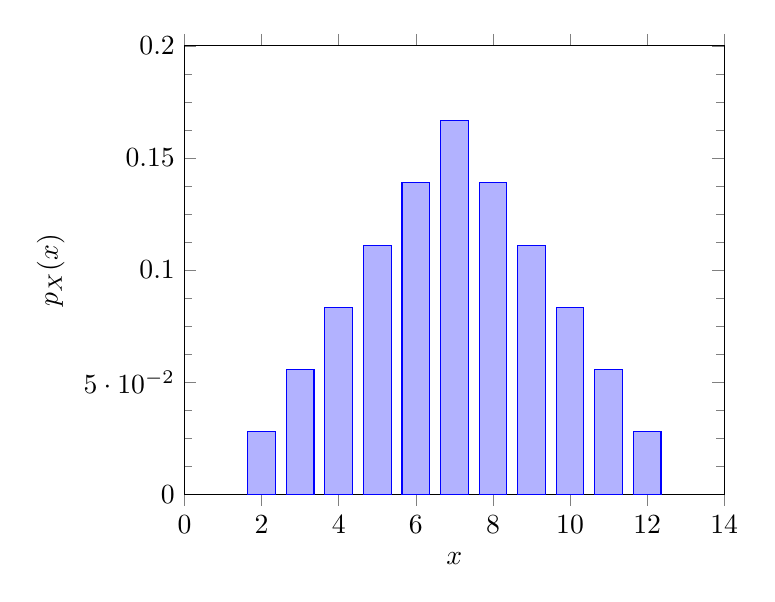
\begin{tikzpicture}
            \begin{axis}[
                ybar,
                xmin = 0, xmax = 14,
                ymin = 0, ymax = 0.2,
                minor y tick num = 3,
                xlabel = {$x$},
                ylabel = {$p_X(x)$},
                ]
                
                \addplot coordinates {
                    (2, 1/36)
                    (3, 2/36) 
                    (4, 3/36) 
                    (5, 4/36) 
                    (6, 5/36) 
                    (7, 6/36) 
                    (8, 5/36) 
                    (9, 4/36) 
                    (10, 3/36) 
                    (11, 2/36) 
                    (12, 1/36) 
                };
            \end{axis}
        \end{tikzpicture}

        \caption{La funzione di massa per la somma di due lanci di un dado.}
        \label{unif_sum}
    \end{figure}
    
    
    Consideriamo ora un'altra funzione $P_X$ descritta come:
    \[P_X(A) = \sum_{x \in A} p_X(x)\]

    Tale funzione viene invece detta \textbf{distribuzione di probabilità} di $X$.
    
    \begin{frameddefn}{Distribuzione di probabilità}
        Data una v.a. discreta $X$, definiamo la distribuzione di probabilità di $X$ come la funzione $P_X : \mathcal{P}(X(\Omega)) \to [0,1] \subset \R$ tale che:
        \[P_X(A) = \sum_{x \in A} p_X(x)\]
    \end{frameddefn}
    
    Prima di tutto, osserviamo che sia facilmente dimostrabile che la tripla $(X(\Omega), \mathcal{P}(X(\Omega)), P_X)$ corrisponda ad un nuovo spazio di probabilità che restringe il nostro interesse unicamente ai valori assumibili dalla v.a. $X$. Successivamente, osserviamo come:
    \[P_X(A) = \Pr[X^{-1}(A)] = \Pr[\{\omega \in \Omega \mid X(\omega) \in A\}]\]

    ossia che $P_X(A)$ corrisponde alla probabilità dell'evento contenente tutti gli esiti che fanno assumere ad $X$ un valore in $A$. In alcune occasioni, scriveremo $\{X \in A\}$ invece di $\{\omega \in \Omega \mid X(\omega) \in A\}$.

    La rappresentazione grafica della funzione di massa e la definizione di distribuzione di probabilità di una v.a. discreta ci permettono di calcolare immediatamente la probabilità di assumere un valore in un insieme determinato.

    Vediamo ora un altro strumento molto utile defininibile tramite la densità discreta: la \textbf{funzione di ripartizione} (o \textit{di distribuzione}) di una variabile aleatoria.
    
    \begin{frameddefn}{Funzione di ripartizione}
        Data una v.a. $X$, definiamo la funzione di ripartizione di $X$ come la funzione $F_X : \R \to [0,1] \subset \R$ tale che:
        \[F_X(x) = \Pr[X \leq x]\]
    \end{frameddefn}
    
    Intuitivamente, l'evento $\{X \leq x\}$ nella definizione riportata sopra corrisponde all'evento $\{\omega \in \Omega \mid X(\omega) \leq x\}$. Inoltre, osserviamo che la definizione data \underline{non sia esclusiva} per le v.a. discrete, bensì sia valida anche per le v.a. continue (torneremo su esse più avanti). Nel caso particolare delle v.a. discrete, notiamo come:
    \[\begin{split}
        F_X(x) &= \Pr[\{\omega \in \Omega \mid X(\omega) \leq x\}] \\
        &= \sum_{\substack{\omega \in \Omega \,:\\ X(\omega) \leq x}} \Pr[\{\omega\}] \\
        &= \sum_{\substack{x \in X(\Omega) \,:\\ x' \leq x}} p_X(x')
    \end{split}\]

    In altre parole, la funzione di ripartizione di una v.a. discreta non è altro che la somma cumulativa delle densità discrete fino ad un certo valore.

    \begin{figure}[H]
        \centering
        \pgfkeys{/pgf/number format/fixed}
        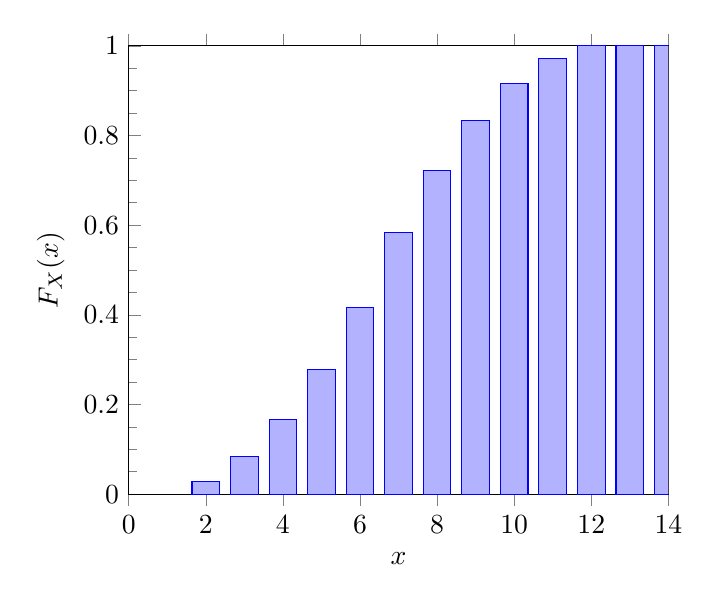
\begin{tikzpicture}
            \begin{axis}[
                ybar,
                xmin = 0, xmax = 14,
                ymin = 0, ymax = 1,
                minor y tick num = 3,
                xlabel = {$x$},
                ylabel = {$F_X(x)$},
                ]
                
                \addplot coordinates {
                    (2, 1/36)
                    (3, 3/36) 
                    (4, 6/36) 
                    (5, 10/36) 
                    (6, 15/36) 
                    (7, 21/36) 
                    (8, 26/36) 
                    (9, 30/36) 
                    (10, 33/36) 
                    (11, 35/36) 
                    (12, 36/36) 
                    (13, 36/36) 
                    (14, 36/36) 
                };
            \end{axis}
        \end{tikzpicture}

        \caption{La funzione di ripartizione per la somma di due lanci di un dado.}
    \end{figure}

    Nel caso particolare delle v.a. discrete a valori interi, dunque le v.a. $X$ con $X(\Omega) \subseteq \Z$, conoscere la funzione di ripartizione è sufficiente a poter ricavare l'intera funzione di massa della variabile stessa. Difatti, dato $k \in \Z$, abbiamo che:
    \[\begin{split}
        p_X(k) &= \Pr[X = k] \\
        &= \Pr[X \leq k] - \Pr[X \leq k-1] \\
        &= F_X(k) - F_X(k-1) 
    \end{split}\]

    In altri casi particolari, se la v.a. (discreta o meno) può assumere un valore minimo $x_{\min}$ e/o un valore massimo $x_{\max}$, dove:
    \[x_{\min} = \min_{\omega \in \Omega} X(\omega) \qquad\qquad x_{\max} = \max_{\omega \in \Omega} X(\omega)\]

    allora avremo che $F_X(x) = 0$ per ogni $x < x_{\min}$ e $F_X(x') = 1$ per ogni $x' \geq x_{\min}$.


    \section{Densità congiunte, condizionate e marginali}

    \label{va_cong_cond_marg}
    Dopo essere tornati dalla loro passeggiata, Marco e Giada decidono di giocare ad un gioco con dadi e monete. In ogni turno del gioco viene lanciato un dado. Il punteggio del turno è definito come l'esito ottenuto dal lancio. Per ogni punto ottenuto, viene lanciata una moneta. Se il numero di teste è superiore al numero di croci, il turno viene vinto da Marco. Viceversa, se il numero di croci è superiore al numero di teste il turno viene vinto da Giada. Nel caso in cui i due numeri siano uguali, il turno finisce in pareggio.

    Essendo molto competitiva, Giada vuole calcolare la sua probabilità di vittoria in un singolo turno. Decidiamo quindi di modellare il problema tramite due variabili aleatorie: la v.a. $X$ che misura il punteggio ottenuto dal lancio del dado e la v.a. $Y$ che misura il numero di lanci di monete con esito croce.
    
    In questo caso, è facile vedere che la variabile $Y$ sia \textbf{dipendente} dalla variabile $X$, poiché il punteggio del dado definisce il numero di monete lanciate. Diamo quindi la definizione di variabili aleatorie discrete indipendenti.

    \begin{frameddefn}{Indipendenza tra v.a. discrete}
        Diciamo che $n$ v.a. discrete $X_1, \ldots, X_n$ sono indipendenti quando per ogni sottoinsieme $I = \{i_1, \ldots, i_k\} \subseteq \{1,\ldots,n\}$ e per ogni $x_{i_1}, \ldots, x_{i_k} \in \R$ si ha che:
        \[\Pr\sbk{\bigcap_{i \in I} X_i = x_i} = \prod_{i \in I} \Pr[X_i = x_i]\]
    \end{frameddefn}
    
    Essendo le due variabili dipendenti, Giada è consapevole che calcolare le sue chance di vittoria, ossia la probabilità dell'evento $\{Y > X/2\}$ non sarà facile. Sfruttando la probabilità totale, Giada ottiene che:
    \[\begin{split}
        \Pr\sbk{Y > \frac{X}{2}} &= \sum_{i = 1}^{6} \Pr\sbk{X = i, Y > \frac{i}{2}} \\
        &= \sum_{i = 1}^{6} \sum_{j = \floor{\frac{i}{2}}+1}^i \Pr[X = i, Y = j] \\
        &= \sum_{i = 1}^{6} \sum_{j = \floor{\frac{i}{2}}+1}^i \Pr[X = i] \Pr[Y = j \mid X = i]\\
    \end{split}\]

    Osserviamo che nel momento in cui il valore di $X = i$ è noto, calcolare la probabilità di ottenere un determinato numero di croci è semplice in quanto si tratta di una probabilità binomiale. Per tanto, concludiamo che:
    \[\begin{split}
        \Pr\sbk{Y > \frac{X}{2}} &= \sum_{i = 1}^{6} \sum_{j = \floor{\frac{i}{2}}+1}^i \frac{1}{6} \binom{i}{j} \rbk{\frac{1}{2}}^i \\
        &= \frac{1}{6} \sum_{i = 1}^{6} \rbk{\frac{1}{2}}^i \rbk{\sum_{j = \floor{\frac{i}{2}}+1}^i \binom{i}{j}} \\
    \end{split}\]

    Non potendo semplificare ulteriormente i conti, a Giada non rimane altro che espandere le due sommatorie annidate e calcolare il valore finale, ottenendo che:
    \[\Pr\sbk{Y > \frac{X}{2}} = \frac{77}{192} \approx 0.4\]

    Per verificare che i suoi conti siano corretti, Giada decide di stendere una tabella che tenga conto di tutti i casi possibili, ossia tutte le probabilità $\Pr[X = x, Y = y]$ per ogni coppia $(x,y) \in X(\Omega) \times Y(\Omega)$.

    \begin{figure}[H]
        \centering

        \resizebox{0.75\textwidth}{!}{
            \begin{tabular}{cc|cccccc}
                & & \multicolumn{6}{c}{$X = x$}{} \\
                & & 1 & 2 & 3 & 4 & 5 & 6 \\
                \hline
                \multirow{7}{*}{\rotatebox{90}{$Y = y$ \hspace{65pt}}}
                & 0 & $\frac{1}{6} \frac{1}{2^1} \binom{1}{0}$  & $\frac{1}{6} \frac{1}{2^2} \binom{2}{0}$  & $\frac{1}{6} \frac{1}{2^3} \binom{3}{0}$  & $\frac{1}{6} \frac{1}{2^4} \binom{4}{0}$  & $\frac{1}{6} \frac{1}{2^5} \binom{5}{0}$  & $\frac{1}{6} \frac{1}{2^6} \binom{6}{0}$  \\[10pt]

                & 1 & $\frac{1}{6} \frac{1}{2^1} \binom{1}{1}$  & $\frac{1}{6} \frac{1}{2^2} \binom{2}{1}$  & $\frac{1}{6} \frac{1}{2^3} \binom{3}{1}$  & $\frac{1}{6} \frac{1}{2^4} \binom{4}{1}$  & $\frac{1}{6} \frac{1}{2^5} \binom{5}{1}$  & $\frac{1}{6} \frac{1}{2^6} \binom{6}{1}$  \\[10pt]

                & 2 & $\frac{1}{6} \frac{1}{2^1} \binom{1}{2}$  & $\frac{1}{6} \frac{1}{2^2} \binom{2}{2}$  & $\frac{1}{6} \frac{1}{2^3} \binom{3}{2}$  & $\frac{1}{6} \frac{1}{2^4} \binom{4}{2}$  & $\frac{1}{6} \frac{1}{2^5} \binom{5}{2}$  & $\frac{1}{6} \frac{1}{2^6} \binom{6}{2}$  \\[10pt]

                & 3 & $\frac{1}{6} \frac{1}{2^1} \binom{1}{3}$  & $\frac{1}{6} \frac{1}{2^2} \binom{2}{3}$  & $\frac{1}{6} \frac{1}{2^3} \binom{3}{3}$  & $\frac{1}{6} \frac{1}{2^6} \binom{4}{3}$  & $\frac{1}{6} \frac{1}{2^5} \binom{5}{3}$  & $\frac{1}{6} \frac{1}{2^6} \binom{6}{3}$  \\[10pt]

                & 4 & $\frac{1}{6} \frac{1}{2^1} \binom{1}{4}$  & $\frac{1}{6} \frac{1}{2^2} \binom{2}{4}$  & $\frac{1}{6} \frac{1}{2^3} \binom{3}{4}$  & $\frac{1}{6} \frac{1}{2^4} \binom{4}{4}$  & $\frac{1}{6} \frac{1}{2^5} \binom{5}{4}$  & $\frac{1}{6} \frac{1}{2^6} \binom{6}{4}$  \\[10pt]

                & 5 & $\frac{1}{6} \frac{1}{2^1} \binom{1}{5}$  & $\frac{1}{6} \frac{1}{2^2} \binom{2}{5}$  & $\frac{1}{6} \frac{1}{2^3} \binom{3}{5}$  & $\frac{1}{6} \frac{1}{2^4} \binom{4}{5}$  & $\frac{1}{6} \frac{1}{2^5} \binom{5}{5}$  & $\frac{1}{6} \frac{1}{2^6} \binom{6}{5}$  \\[10pt]

                & 6 & $\frac{1}{6} \frac{1}{2^1} \binom{1}{6}$  & $\frac{1}{6} \frac{1}{2^2} \binom{2}{6}$  & $\frac{1}{6} \frac{1}{2^3} \binom{3}{6}$  & $\frac{1}{6} \frac{1}{2^4} \binom{4}{6}$  & $\frac{1}{6} \frac{1}{2^5} \binom{5}{6}$  & $\frac{1}{6} \frac{1}{2^6} \binom{6}{6}$  \\[10pt]

            \end{tabular}
        }

        \caption{Funzione di massa di $\Pr[X = x, Y = y]$}
    \end{figure}

    Implicitamente, Giada non ha fatto altro che calcolare la \textbf{densità discreta congiunta} delle variabili $X$ ed $Y$.
    
    \begin{frameddefn}{Densità discreta congiunta}
        Date due v.a. discrete $X$ ed $Y$, definiamo la densità discreta congiunta di $X$ ed $Y$ come la funzione $p_{X,Y} : \R^2 \to [0,1] \subset \R$ tale che:
        \[p_{X,Y}(x,y) = \Pr[X=x, Y=y]\]
    \end{frameddefn}
    
    Una volta computati i valori della tabella, Giada può calcolare la probabiltà dell'evento che descrive la sua vittoria, ossia l'evento  $\{Y > X/2\}$, sommando le densità congiunte di tutte le coppie $x,y$ per cui $y > x/2$, confermando che:
    \[\Pr\sbk{Y > \frac{X}{2}} = \frac{77}{192}\]

    \begin{figure}[H]
        \centering

        \resizebox{0.45\textwidth}{!}{
            \begin{tabular}{cc|cccccc}
                & & \multicolumn{6}{c}{$X = x$}{} \\
                & & 1 & 2 & 3 & 4 & 5 & 6 \\
                \hline
                \multirow{7}{*}{\rotatebox{90}{$Y = y$ \hspace{65pt}}}
                & 0 & $\frac{1}{12}$  & $\frac{1}{24}$  & $\frac{1}{48}$  & $\frac{1}{96}$  & $\frac{1}{192}$  & $\frac{1}{384}$  \\[10pt]

                & 1 & \cellcolor[HTML]{ccccff}$\frac{1}{12}$ & $\frac{2}{24}$  & $\frac{3}{48}$  & $\frac{4}{96}$  & $\frac{5}{192}$  & $\frac{6}{384}$  \\[10pt]

                & 2 & \cellcolor[HTML]{ccccff}$0$  & \cellcolor[HTML]{ccccff}$\frac{1}{24}$  & \cellcolor[HTML]{ccccff}$\frac{3}{48}$  & $\frac{6}{96}$  & $\frac{10}{192}$  & $\frac{15}{384}$  \\[10pt]

                & 3 & \cellcolor[HTML]{ccccff}$0$  & \cellcolor[HTML]{ccccff}$0$  & \cellcolor[HTML]{ccccff}$\frac{1}{48}$  & \cellcolor[HTML]{ccccff}$\frac{4}{96}$  & \cellcolor[HTML]{ccccff}$\frac{10}{192}$  & $\frac{20}{384}$  \\[10pt]

                & 4 & \cellcolor[HTML]{ccccff}$0$  & \cellcolor[HTML]{ccccff}$0$  & \cellcolor[HTML]{ccccff}$0$  & \cellcolor[HTML]{ccccff}$\frac{1}{96}$  & \cellcolor[HTML]{ccccff}$\frac{5}{192}$  & \cellcolor[HTML]{ccccff}$\frac{15}{384}$  \\[10pt]

                & 5 & \cellcolor[HTML]{ccccff}$0$  & \cellcolor[HTML]{ccccff}$0$  & \cellcolor[HTML]{ccccff}$0$  & \cellcolor[HTML]{ccccff}$0$  & \cellcolor[HTML]{ccccff}$\frac{1}{192}$  & \cellcolor[HTML]{ccccff}$\frac{6}{384}$  \\[10pt]

                & 6 & \cellcolor[HTML]{ccccff}$0$  & \cellcolor[HTML]{ccccff}$0$  & \cellcolor[HTML]{ccccff}$0$  & \cellcolor[HTML]{ccccff}$0$  & \cellcolor[HTML]{ccccff}$0$  & \cellcolor[HTML]{ccccff}$\frac{1}{384}$  \\[10pt]

            \end{tabular}
        }

        \caption{La somma tra le probabilità evidenziate di azzurro corrisponde a $\Pr[Y > X/2]$}
    \end{figure}

    Tabelle che esprimono a pieno la densità congiunta di due variabili risultano estremamente utili per osservare l'interazione tra le due variabili. Tipicamente, esse vengono estese anche con le \textbf{probabilità marginali} delle due variabili, cioè le loro probabilità totali ottenute fissando un valore per una delle due variabili e sommando tutte le probabilità congiunte per tutti i valori assumibili dall'altra variabile. Ad esempio, la probabilità marginale dell'evento $\{Y = y\}$ è data da:
    \[\Pr[Y = y] = \sum_{x \in X(\Omega)} \Pr[X = x, Y = y]\]

    Osserviamo che tali probabilità marginali sono facilmente computabili tramite la tabella riportata. Ad esempio, per ogni $y \in Y(\Omega)$, possiamo calcolare $\Pr[Y = y]$ sommando l'intera riga del valore $y$. Viceversa, per ogni $x \in X(\Omega)$ possiamo calcolare $\Pr[X = x]$ sommando l'intera colonna del valore $x$.

    \begin{figure}[H]
        \centering

        \resizebox{0.5\textwidth}{!}{
            \begin{tabular}{cc|cccccc|c}
                & & \multicolumn{6}{c|}{$X = x$} & \\
                & & 1 & 2 & 3 & 4 & 5 & 6 \\
                \hline
                \multirow{7}{*}{\rotatebox{90}{$Y = y$ \hspace{65pt}}}
                & 0 & $\frac{1}{12}$  & $\frac{1}{24}$  & $\frac{1}{48}$  & $\frac{1}{96}$  & $\frac{1}{192}$  & $\frac{1}{384}$  & $\frac{21}{128}$\\[10pt]

                & 1 & $\frac{1}{12}$ & $\frac{2}{24}$  & $\frac{3}{48}$  & $\frac{4}{96}$  & $\frac{5}{192}$  & $\frac{6}{384}$  & $\frac{5}{16}$\\[10pt]

                & 2 & $0$  & $\frac{1}{24}$  & $\frac{3}{48}$  & $\frac{6}{96}$  & $\frac{10}{192}$  & $\frac{15}{384}$  & $\frac{33}{128}$\\[10pt]

                & 3 & $0$  & $0$  & $\frac{1}{48}$  & $\frac{4}{96}$  & $\frac{10}{192}$  & $\frac{20}{384}$ & $\frac{1}{6}$ \\[10pt]

                & 4 & $0$  & $0$  & $0$  & $\frac{1}{96}$  & $\frac{5}{192}$  & $\frac{15}{384}$  & $\frac{29}{384}$\\[10pt]

                & 5 & $0$  & $0$  & $0$  & $0$  & $\frac{1}{192}$  & $\frac{6}{384}$  & $\frac{17}{384}$\\[10pt]

                & 6 & $0$  & $0$  & $0$  & $0$  & $0$  & $\frac{1}{384}$  & $\frac{1}{184}$\\[10pt]
                \hline

                &  & $\frac{1}{6}$  & $\frac{1}{6}$  & $\frac{1}{6}$  & $\frac{1}{6}$  & $\frac{1}{6}$  & $\frac{1}{6}$  & $1$ \\[10pt]

            \end{tabular}
        }

        \caption{Estensione della tabella con le sue probabilità marginali.}
    \end{figure}

    Notiamo inoltre che tale tabella possa essere utilizzata anche per calcolare la \textbf{densità discreta condizionata} delle variabili $X$ ed $Y$.

    \begin{frameddefn}{Densità discreta condizionata}
        Date due v.a. discrete $X$ ed $Y$, definiamo la densità discreta condizionata di $X$ su $Y$ come la funzione $p_{X \mid Y} : \R^2 \to [0,1] \subset \R$ tale che:
        \[p_{X \mid Y}(x \mid y) = \Pr[X=x \mid Y=y]\]
    \end{frameddefn}

    Per definizione, sappiamo che:
    \[\Pr[X = x \mid Y = y] = \frac{\Pr[X = x, Y = y]}{\Pr[Y = y]}\]

    Ciò implica che per calcolare la densità $p_{X \mid Y}$ è sufficiente dividere ogni cella della tabella per la probabilità marginale dell'evento il cui esito è già saputo. Ad esempio, nella tabella riportata precedentemente è sufficiente dividere il valore della cella $(0,1)$ per la probabilità marginale della 0-esima riga al fine di ottenere il valore di $p_{X \mid Y}(1 \mid 0)$:
    \[p_{X \mid Y}(1 \mid 0) = \frac{p_{X,Y}(1,0)}{p_{Y}(0)} = \frac{1}{12} \frac{128}{21} = \frac{32}{63}\]

    Per le densità discrete congiunte possiamo individuare anche un analogo $F_{X,Y}$ della funzione di ripartizione, definita come:
    \[F_{X,Y}(x,y) = \Pr[X \leq x, Y \leq y] \]

    Evidenziamo alcune proprietà banali di tale funzione di ripartizione, ossia:
    \[\begin{split}
        \lim_{x \to -\infty} F_{X,Y}(x,y) = 0 \quad&\quad \lim_{y \to -\infty} F_{X,Y}(x,y) = 0 \\
        \lim_{x \to +\infty} F_{X,Y}(x,y) = F_{Y}(y) \quad&\quad \lim_{y \to +\infty} F_{X,Y}(x,y) = F_X(x) \\
    \end{split}\]

    Proprietà meno scontata è la possibilità di esprimere la funzione di ripartizione congiunta come prodotto delle due funzioni di ripartizione. Intuitivamente, ciò risulta certamente vero se le due v.a. sono \underline{indipendenti}. Difatti, abbiamo che:
    \[\begin{split}
        F_{X,Y}(x,y) &= \Pr[X \leq x, Y \leq y]\\
        &= \sum_{\substack{x' \in X(\Omega) \,: \\ x' \leq x}}  \sum_{\substack{y' \in Y(\Omega) \,: \\ y' \leq y}} \Pr[X = x, Y = y] \\
        &= \sum_{\substack{x' \in X(\Omega) \,: \\ x' \leq x}}  \sum_{\substack{y' \in Y(\Omega) \,: \\ y' \leq y}} \Pr[X = x] \Pr[Y = y] \\
        &= \sum_{\substack{x' \in X(\Omega) \,: \\ x' \leq x}} \Pr[X = x] \rbk{\sum_{\substack{y' \in Y(\Omega) \,: \\ y' \leq y}}  \Pr[Y = y]} \\
        &= \Pr[Y \leq y] \sum_{\substack{x' \in X(\Omega) \,: \\ x' \leq x}} \Pr[X = x] \\
        &= \Pr[Y \leq y] \Pr[X \leq x] \\
        &= F_X(x) F_Y(y) \\
    \end{split}\]

    Per quanto riguarda v.a. dipendenti, invece, risulta diretto chiedersi se valga l'opposto, vale a dire se l'egualianza non valga mai. A questa domanda, la risposta è negativa.

    \section{Distribuzioni discrete note}

    \subsection{Distribuzione uniforme, degenere e di Bernoulli}

    Dopo aver introdotto il concetto generale di variabile aleatoria, vediamo alcuni esempi di \textbf{distribuzioni note}, ossia distribuzioni che vengono frequentemente utilizzate per modellare problemi. L'utilizzo di distribuzioni note ci permette di astrarre ulteriormente il concetto di probabilità: invece di ragionare sulla probabilità con cui calcolare un'incertezza matematica, ci basta ragionare su che tipo di distribuzione corrisponda al problema ed applicare ciò che è già noto della distribuzione scelta. Per ora, continueremo a concentrarci solo ed esclusivamente su variabili aleatorie discrete.

    Il primo tipo di distribuzione discreta nota che vedremo è anche il più semplice ed immediato. Come suggerisce il nome, la \textbf{distribuzione uniforme discreta} descrive una variabile aleatoria la cui probabilità è \textit{uniforme} su un intervallo $\{a, \ldots, b\} \subset \Z$ con $a \leq b$, ossia non esistono valori più \curlyquotes{probabili} di altri: tutti i punti dell'intervallo sono equiprobabili tra loro. Formalmente, la funzione di massa di una v.a. discreta $X$ a distribuzione uniforme sull'intervallo $\{a,\ldots, b\} \subset \Z$ è definita come:
    \[p_X(x) = \soe{ll}{
        \frac{1}{b-(a-1)} & \text{se } a \leq x \leq b \\
        0 & \text{altrimenti}
    }\]

    in modo tale che:
    \[\sum_{k = a}^b \Pr[X = k] = \sum_{k = a}^b \frac{1}{b-(a-1)} = \frac{b-(a-1)}{b-(a-1)} = 1\]

    \begin{frameddefn}{Distribuzione uniforme discreta}
        Una v.a. $X$ è detta a distribuzione uniforme discreta di parametri $a$ e $b$, indicato con $X \sim \mathcal{U}\{a,b\}$, quando tutti i valori dell'intervallo $[a,b] \subset \Z$ sono equiprobabilmente assumibili da $X$.

        Per ogni v.a $X \sim \mathcal{U}\{a,b\}$ vale che:
        \begin{itemize}
            \item $X(\Omega) = \{a, \ldots, b\}$
            \item La funzione di massa è dettata da:
            \[p_X(x) = \soe{ll}{
                \frac{1}{b-(a-1)} & \text{se } a \leq x \leq b \\
                0 & \text{altrimenti}
            }\]
        \end{itemize}
    \end{frameddefn}

    \begin{figure}[H]
        \centering
        \resizebox{0.6\textwidth}{!}{
            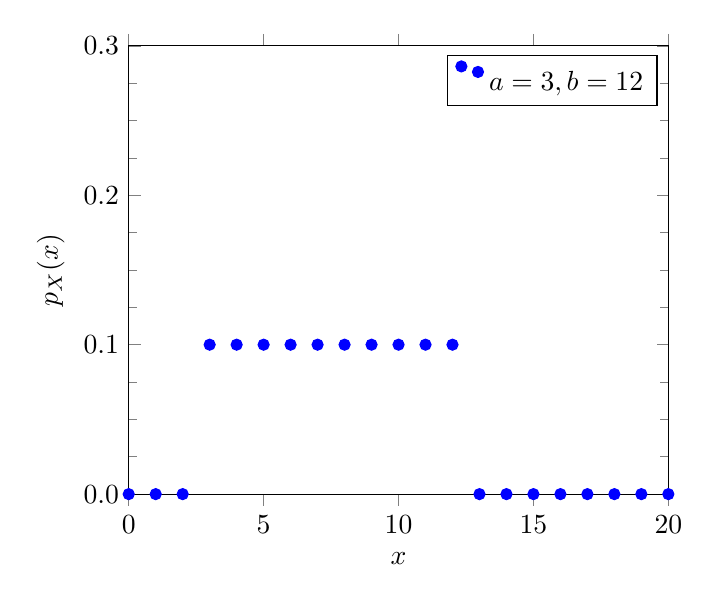
\begin{tikzpicture}[
                declare function={uniform(\x,\xl,\xu)= (\x>=\xl)*(\x<=\xu)*1/(\xu-\xl+1);}
            ]
                \begin{axis}[
                    ybar,
                    xmin = 0, xmax = 20,
                    ymin = 0, ymax = 0.3,
                    minor y tick num = 3,
                    xlabel = {$x$},
                    ylabel = {$p_X(x)$},
                    samples at={0,...,20},
                    yticklabel style={
                        /pgf/number format/fixed,
                        /pgf/number format/fixed zerofill,
                        /pgf/number format/precision=1
                    }
                    ]

                \addplot [only marks, blue] {uniform(x,3,12)}; \addlegendentry{$a = 3, b = 12$}
                \end{axis}
            \end{tikzpicture}
        }

        \caption{Funzioni di massa di una distribuzione uniforme discreta.}
    \end{figure}
    
    Quando una $a = b$ in una distribuzione uniforme, l'intera probabilità è accentrata verso un singolo valore. Chiaramente, ogni variabile aleatoria per cui $\abs{X(\Omega)} = 1$ corrisponde ad un'uniforme discreta con estremi coincidenti in $x_0$. Una distribuzione di questo tipo viene detta \textbf{distribuzione degenere}.

    \begin{frameddefn}{Distribuzione degenere}
        Una v.a. $X$ è detta a distribuzione degere se $X(\Omega) = \{x_0\}$.
    \end{frameddefn}

    Visto che essa può assumere un solo valore, la funzione di massa di ogni v.a. degenere $X$ con $X(\Omega) = \{x_0\}$ concentra tutta la probabilità verso il valore $x$, ossia:
    \[\Pr[X = x_0] = 1 \qquad \Pr[X \neq x_0] = 0\]

    Osserviamo quindi che la funzione di massa possa essere descritta completamente da una semplice \textbf{funzione indicatrice} $\1_{\{x_0\}}(x)$, dove per ogni $A \subseteq \Omega$ si ha che:
    \[\1_{A}(x) = \soe{ll}{
        1 & \text{se } x \in A \\
        0 & \text{se } x \notin A \\
    }\]

    Per questo motivo, è di comune uso utilizzare direttamente una funzione indicatrice al posto di tali variabili aleatorie.

    Il secondo tipo di distribuzione nota che introduciamo è la \textbf{distribuzione di Bernoulli}. Questa distribuzione modella tutti i processi che danno luce a solo ed esclusivamente due possibilità: un \textit{successo} (indicato con 1) e un \textit{fallimento} (indicato con 0).

    \begin{frameddefn}{Distribuzione di Bernoulli}
        Una v.a. $X$ è detta a distribuzione di Bernoulli di parametro $p$, indicato con $X \sim \mathcal{B}(p)$, quando:
        \begin{itemize}
            \item $X(\Omega) = \{0,1\}$
            \item La funzione di massa è dettata da:
            \[p_X(k)  = \soe{ll}{
                p & \text{se } k = 1 \\
                1-p & \text{se } k = 0 \\
            }\]
        \end{itemize}
    \end{frameddefn}
    
    Osserviamo che le distribuzioni di Bernoulli possono essere utilizzate per modellare \underline{ogni} processo stocastico che può assumere solo due valori generici $a$ e $b$ e non unicamente i valori $0$ ed $1$. Ad esempio, per descrivere la v.a. discreta $Y$ tale che $Y(\Omega) = \{a,b\}$ e con funzione di massa dettata da $p_Y(a) = p$ e $p_Y(b) = 1-p$ in termini di distribuzione di Bernoulli, possiamo definire una nuova v.a. $X \sim \mathcal{B}(p)$ per poi porre semplicemente $Y = (a-b)X + b$. In questo modo, si ha che:
    \[\Pr[Y = a] = \Pr[(a-b)X + b = a] = \Pr[(a-b)X = a-b] = \Pr[X = 1] = p\]
    \[\Pr[Y = b] = \Pr[(a-b)X + b = b] = \Pr[(a-b)X = 0] = \Pr[X = 0] = 1-p\]

    Similmente, le distribuzioni di Bernoulli possono anche essere utilizzate per modellare le distribuzioni degeneri. Ad esempio, la distribuzione $\1_{\{x_0\}}(x)$ con $x_0 \neq 0$ può essere modellata da una variabile $Y' = x_0X'$ con $X' \sim \mathcal{B}(1)$:
    \[\Pr[Y' = x_0] = \Pr[x_0X' = x_0] = \Pr[X' = 1] = 1\]
    \[\Pr[Y' \neq x_0] = \Pr[x_0X' \neq x_0] = \Pr[X' = 0] = 0\]

    Per $x_0 = 0$, invece, possiamo definire una variabile $Y'' = 1-X''$ con $X'' \sim \mathcal{B}(1)$:
    \[\Pr[Y'' = 0] = \Pr[1-X'' = 0] = \Pr[X'' = 1] = 1\]
    \[\Pr[Y'' \neq 0] = \Pr[1-X'' \neq 0] = \Pr[X'' \neq 1] = 0\]

    \subsection{Distribuzione binomiale e geometrica}

    Come mostrato nella sezione precedente, la distribuzione di Bernoulli risulta fondamentale nel calcolo delle probabilità. Essa ci permette comodamente di modellare una molteplicità infinita di processi stocastici detti \textbf{processi di Bernoulli}. Un processo di Bernoulli è una successione di $n$ v.a. \textbf{indipendenti ed identicamente distribuite (i.i.d.)} $X_1, \ldots, X_n \sim \mathcal{B}(p)$ dette \textit{prove di Bernoulli}. Tipicamente, siamo interessati a sapere informazioni come la probabilità che vi siano $k$ successi o la probabilità che il primo successo si verifichi al $t$-esimo tentativo.
    
    Nel primo problema, possiamo modellare il numero di successi come una v.a. $X$ corrispondente alla somma degli esiti di tutte le prove, ossia $X = X_1 + \ldots + X_n$.  Risulta evidente che la probabilità $\Pr[X = k]$, con $k \in \{0, \ldots, n\}$, corrisponde ad una probabilità binomiale:
    \[\Pr[X = k] = \Pr[X_1 + \ldots + X_n = k] = \binom{n}{k} p^k (1-p)^{n-k}\]

    Tale distribuzione è anch'essa nota ed è detta \textbf{distribuzione binomiale}, la quale modella il numero di successi in un processo di Bernoulli.

    \begin{frameddefn}{Distribuzione binomiale}
        Una v.a. $X$ è detta a distribuzione binomiale di parametri $n$ e $p$, indicato con $X \sim \mathrm{Bin}(n,p)$, quando $X = X_1+\ldots + X_n$ per $X_1, \ldots, X_n \sim \mathcal{B}(p)$.

        Per ogni v.a $X \sim \mathrm{Bin}(n,p)$ vale che:
        \begin{itemize}
            \item $X(\Omega) = \{0,\ldots,n\}$ con $n\in \N$ e $p \in [0,1] \subset \R$
            \item La funzione di massa è dettata da:
            \[p_X(k)  = \binom{n}{k} p^k (1-p)^k\]
        \end{itemize}
    \end{frameddefn}

    \begin{figure}[H]
        \centering
        \resizebox{0.6\textwidth}{!}{
            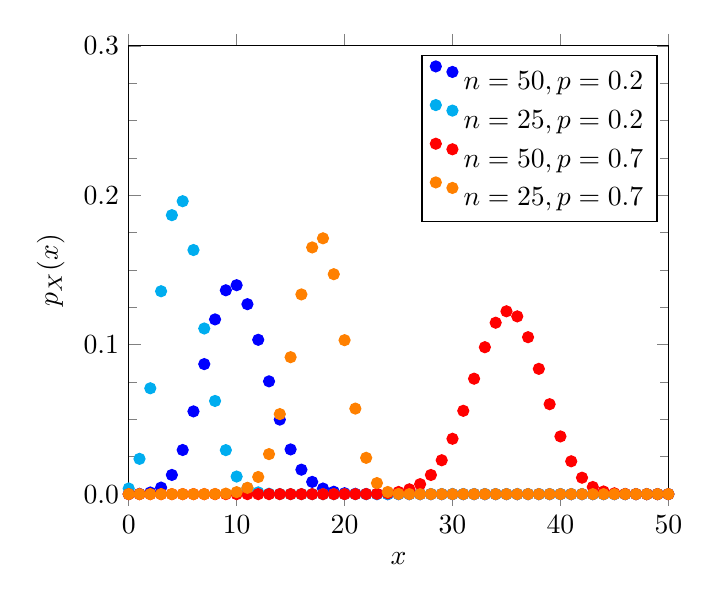
\begin{tikzpicture}[
                declare function={binom(\k,\n,\p)=\n!/(\k!*(\n-\k)!)*\p^\k*(1-\p)^(\n-\k);}
            ]
                \begin{axis}[
                    ybar,
                    xmin = 0, xmax = 50,
                    ymin = 0, ymax = 0.3,
                    minor y tick num = 3,
                    xlabel = {$x$},
                    ylabel = {$p_X(x)$},
                    samples at={0,...,50},
                    yticklabel style={
                        /pgf/number format/fixed,
                        /pgf/number format/fixed zerofill,
                        /pgf/number format/precision=1
                    }
                    ]

                    \addplot [only marks, blue] {binom(x,50,0.2)}; \addlegendentry{$n = 50, p=0.2$}
                    \addplot [only marks, cyan] {binom(x,25,0.2)}; \addlegendentry{$n = 25, p=0.2$}
                    \addplot [only marks, red] {binom(x,50,0.7)}; \addlegendentry{$n = 50, p=0.7$}
                    \addplot [only marks, orange] {binom(x,25,0.7)}; \addlegendentry{$n = 25, p=0.7$}
                \end{axis}
            \end{tikzpicture}
        }

        \caption{Funzioni di massa di quattro distribuzioni binomiali.}
    \end{figure}

    Nel secondo problema, per definizione stessa il primo successo potrebbe verificarsi dopo un numero indeterminato di prove. Questo implica che il processo descrivente il problema deve essere descritto da una successione infinita di prove $Y_1, Y_2, \ldots \sim \mathcal{B}(p)$. Possiamo modellare il primo successo come una v.a. $Y$ il cui valore corrisponde al minimo indice in $\N$ per cui si ha un successo.
    \[Y = \min\{i \in \N-\{0\} \mid Y_i = 1\}\]

    Osserviamo quindi che, essendo $Y_1, Y_2, \ldots$ i.i.d., per $k \in \N-\{0\}$ vale che:
    \[\begin{split}
        \Pr[Y = k] &= \Pr[Y_1 = 0, \ldots, Y_{k-1} = 0, Y_k = 1] \\
        &= \Pr[Y_1 = 0] \cdot \ldots \cdot \Pr[Y_{k-1} = 0] \Pr[Y_k = 1]\\
        &= (1-p)^k p
    \end{split}\]

    \begin{frameddefn}{Distribuzione geometrica}
        Una v.a. $X$ è detta a distribuzione geometrica di parametro $p$, indicato con $X \sim \mathrm{Geom}(p)$, quando $X = \min\{i \in \N-\{0\} \mid X_i = 1\}$ per $X_1, X_2, \ldots \sim \mathcal{B}(p)$.

        Per ogni v.a $X \sim \mathrm{Geom}(p)$ vale che:
        \begin{itemize}
            \item $X(\Omega) = \N-\{0\}$ e $p \in [0,1] \subset \R$
            \item La funzione di massa è dettata da:
            \[p_X(k) = (1-p)^{k-1} p\]
        \end{itemize}
    \end{frameddefn}

    \begin{figure}[H]
        \centering
        \resizebox{0.6\textwidth}{!}{
            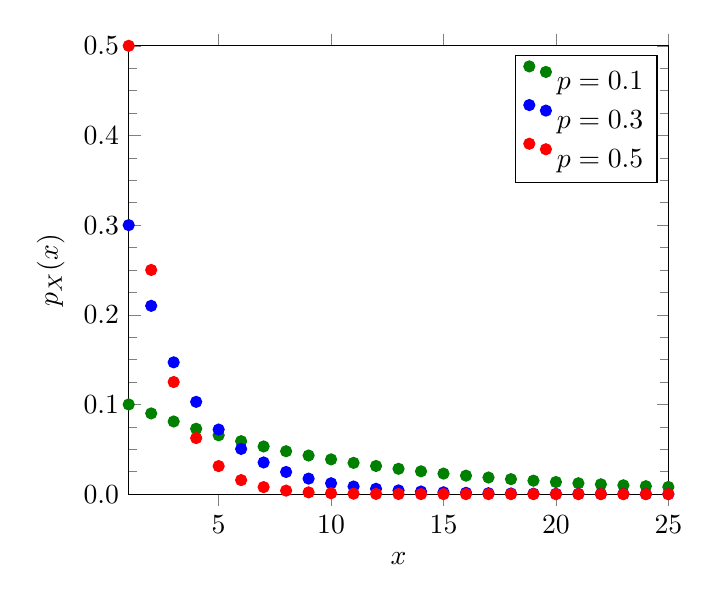
\begin{tikzpicture}[
                declare function={geo(\k,\p)=(1-\p)^(\k-1)*\p;}
            ]
                \begin{axis}[
                    ybar,
                    xmin = 1, xmax = 25,
                    ymin = 0, ymax = 0.5,
                    minor y tick num = 3,
                    xlabel = {$x$},
                    ylabel = {$p_X(x)$},
                    samples at={1,...,25},
                    yticklabel style={
                        /pgf/number format/fixed,
                        /pgf/number format/fixed zerofill,
                        /pgf/number format/precision=1
                    }
                    ]

                    \addplot [only marks, Green] {geo(x,0.1)}; \addlegendentry{$p=0.1$}
                    \addplot [only marks, blue] {geo(x,0.3)}; \addlegendentry{$p=0.3$}
                    \addplot [only marks, red] {geo(x,0.5)}; \addlegendentry{$p=0.5$}
                \end{axis}
            \end{tikzpicture}
        }

        \caption{Funzioni di massa di tre distribuzioni geometriche.}
    \end{figure}

    \subsection{Distribuzione ipergeometrica}

    A questo punto risulta naturale chiedersi se anche la probabilità ipergeometrica già incontrata in precedenza possa essere descritta come un processo di Bernoulli. In questo caso, la risposta è negativa: ogni estrazione è dipendente da quelle precedenti poiché potrebbero aver tolto o meno degli elementi di nostro interesse. In particolare, dati $N$ esiti totali di cui $K \leq N$ positivi, se $X$ è il numero di esiti positivi tra $n \leq K$ esiti scelti a caso degli $N$ totali allora possiamo descrivere $X$ come $X = X_1 + \ldots + X_n$, dove $\forall i \in \{1, \ldots, n\}$ abbiamo:
    \[X_i \sim \mathcal{B}\rbk{\frac{K-\sum_{j = 1}^{i-1} X_j}{N-(i-1)}}\]

    Risulta evidente che trovare una formula chiusa per la densità discreta assunta da $X$ per ogni valore $k \in \{0, \ldots, K\}$. Cerchiamo quindi un'altra strada.

    Siano quindi $X'_1, \ldots, X'_N$ le $N$ prove di Bernoulli effettuate, ognuna dipendente dalle precedenti. Dato $I = \{1, \ldots, N\}$, sia $T = \{i \in I \mid X'_i = 1\}$ l'insieme di successi totali, dove $\abs{T_1} = K$. Sia inoltre $S \subseteq I$ il sottoinsieme degli indici delle prove prese in analisi tra le $N$ totali, dove $\abs{S} = n$.

    Per ogni $i \in I$, siano $Y_i$ e $Z_i$ le v.a. definite come $Y_i = \1_{T}(i)$ e $Z_i =\1_{S}(i)$. Per i vincoli del problema, abbiamo che:
    \[\sum_{i = 1}^N Y_i = K \qquad \sum_{i = 1}^N Z_i = n\]

    Tramite le v.a. appena definite, possiamo definire $X$ come:
    \[X = \sum_{i = 1}^N Y_iZ_i\]

    Per ottenre la densità di $X$, è necessario svolgere alcune manipolazioni algebriche non banali. Sia $A$ l'evento definito come:
    \[A \equiv \cbk{\sum_{i = 1}^N Y_i = K, \sum_{i = 1}^N Z_i = n}\]

    Abbiamo che:
    \[\begin{split}
        \Pr[X = x] &= \Pr\sbk{\left . \sum_{i = 1}^N Y_iZ_i = k \, \right | A} \\
        &= \sum_{z_1, \ldots, z_N \in \{0,1\}^N} \Pr\sbk{\left . \sum_{i = 1}^N Y_iZ_i = k \, \right | \forall i \in I \; Z_i = z_i, A } \Pr\sbk{\forall i \in I \; Z_i = z_i \left | A \right .}\\
        &= \frac{1}{\binom{N}{n}} \sum_{z_1, \ldots, z_N \in \{0,1\}^N} \Pr\sbk{\left . \sum_{i = 1}^N Y_iZ_i = k \, \right | \forall i \in I \; Z_i = z_i, A} \\
        &= \frac{1}{\binom{N}{n}} \sum_{z_1, \ldots, z_N \in \{0,1\}^N} \Pr\sbk{\left . \sum_{i = 1}^N Y_iZ_i = k \, \right | \forall i \in I \; Z_i = z_i, A} \\
        &= \frac{1}{\binom{N}{n}} \binom{K}{k} \binom{N-K}{n-k} \\
    \end{split}\] 

    \begin{frameddefn}{Distribuzione ipergeometrica}
        Una v.a. $X$ è detta a distribuzione ipergeometrica di parametri $N,K,n$, indicato con $X \sim \mathrm{Hyp}(N,K,n)$, quando $X$ descrive il numero di esiti positivi tra $n$ esiti scelti da $N$ totali sapendo che $K$ degli $N$ totali sono positivi.

        Per ogni v.a $X \sim \mathrm{Hyp}(N,K,n)$ vale che:
        \begin{itemize}
            \item $N,K,n \in \N$ con $0 \leq n,K \leq N$
            \item $X(\Omega) = \{0, \ldots, K\}$
            \item La funzione di massa è dettata da:
            \[p_X(k)  = \frac{\binom{K}{k} \binom{N-K}{n-k}}{\binom{N}{n}} \]
            per $0 \leq k \leq n,K$, altrimenti 0.
        \end{itemize}
    \end{frameddefn}

    \begin{figure}[H]
        \centering
        \resizebox{0.6\textwidth}{!}{
            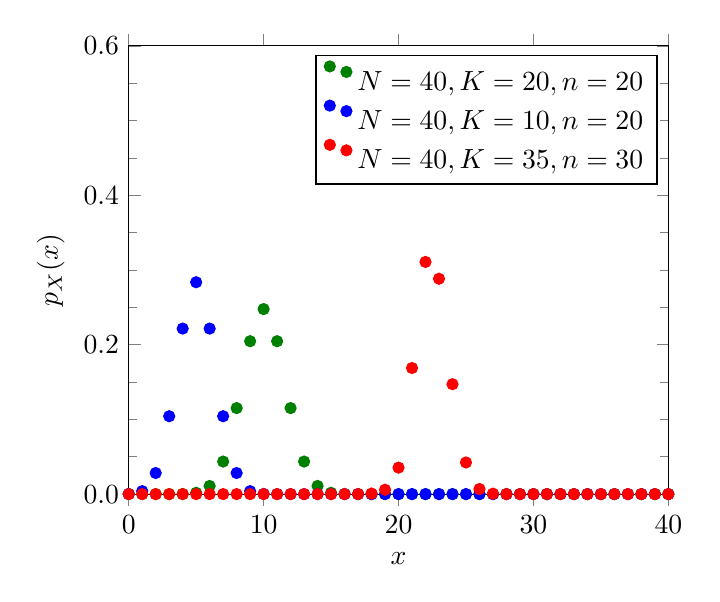
\begin{tikzpicture}[
                declare function={
                    hyp(\k,\N,\K,\n) = (\K!/(\k!*(\K-\k)!)*((\N-\K)!/((\n-\k)!*(\N-\K-\n+\k)!)))/(\N!/(\n!*(\N-\n)!));
                }
            ]
                \begin{axis}[
                    ybar,
                    xmin = 0, xmax = 40,
                    ymin = 0, ymax = 0.6,
                    minor y tick num = 3,
                    xlabel = {$x$},
                    ylabel = {$p_X(x)$},
                    samples at={0,...,40},
                    yticklabel style={
                        /pgf/number format/fixed,
                        /pgf/number format/fixed zerofill,
                        /pgf/number format/precision=1
                    }
                    ]

                    \addplot [only marks, Green] {hyp(x,40,20,20)}; \addlegendentry{$N = 40, K=20, n=20$}
                    \addplot [only marks, blue] {hyp(x,40,10,20)}; \addlegendentry{$N = 40, K=10, n=20$}
                    \addplot [only marks, red] {hyp(x,40,30,30)}; \addlegendentry{$N = 40, K=35, n=30$}
                \end{axis}
            \end{tikzpicture}
        }

        \caption{Funzioni di massa di tre distribuzioni ipergeometriche.}
    \end{figure}

    \subsection{Distribuzione di Poisson}

    Abbiamo visto come la distribuzione binomiale descrive il numero di successi all'interno di un processo di Bernoulli formato da $n$ prove indipendenti, ognuna con probabilità di successo $p$. In molti casi pratici, la distriuzione binomiale può diventa \curlyquotes{pesante} per via dei parametri in gioco. Ad esempio, in numerose applicazioni (come il numero di difetti in un prodotto, visti come un successo in questo caso, o il numero di telefonate ricevute da un call-center in un minuto), abbiamo un numero di prove $n$ molto grande e una probabilità di successo $p$ molto piccola.
    
    In questi casi, calcolare la probabilità binomiale diventa molto scomodo: si pensi banalmente al fatto che per valori di $n$ molto grandi il coefficiente binomiale all'interno del calcolo tenda ad \curlyquotes{esplodere}. Cerchiamo quindi un modello più semplice che vada ad approssimare il comportamento di tali processo stocastici.

    Consideriamo la v.a. binomiale $X \sim B(n,p)$ con un valore di $n$ è un numero molto grande e $p$ un numero molto piccolo (dunque con $n \to +\infty$ e con $p \to 0$). Sia $\lambda$ il valore definito come $\lambda = np$. Osserviamo che:
    \[\begin{split}
        p_X(k) &= \binom{n}{k} p^k (1-p)^{n-k} \\
        &= \frac{n!}{(n-k)! \cdot k!} \left ( \frac{\lambda}{n}\right )^k \left (1- \frac{\lambda}{n}\right )^{n-k} \\
        &= \frac{n!}{(n-k)! \cdot k! } \rbk{\frac{\lambda^k}{n^k}} \left (1- \frac{\lambda}{n}\right )^{n} \left (1- \frac{\lambda}{n}\right )^{-k}
    \end{split} \]

    A questo punto, osserviamo che per $n \to +\infty$ si abbia che:
    \[ \lim_{n \to +\infty} \left (1- \frac{\lambda}{n}\right )^n = e^{-\lambda}\]
    \[\lim_{n \to +\infty} \left (1- \frac{\lambda}{n}\right )^{-k} = (1-0)^{-k} = 1\]
    \[\lim_{n \to +\infty} \frac{n!}{(n-k)! \cdot n^k} = \lim_{n \to +\infty} \frac{n \cdot (n-1) \cdot \ldots \cdot (n-k+1)}{n^k} = 1\]

    Concludiamo quindi che:    
    \[ \lim_{n \to +\infty} P_X(k) = \lim_{n \to +\infty} \frac{n!}{(n-k)! \cdot k! } \rbk{\frac{\lambda^k}{n^k}} \left (1- \frac{\lambda}{n}\right )^{n} \left (1- \frac{\lambda}{n}\right )^{-k} = e^{-\lambda} \frac{\lambda^k}{k!}\]

    La variabile aleatoria descritta da tale densità viene detta a \textbf{distribuzione di Poisson} (o anche \textit{distribuzione ad eventi rari}).

    \begin{frameddefn}{Distribuzione di Poisson}
        Una v.a. $X$ è detta a distribuzione di Poisson di parametro $\lambda$, indicato con $X \sim \mathrm{Poiss}(\lambda)$, quando $X$ descrive il numero di successi che si verificano molto raramente ed indipendentemente in un dato intervallo di tempo.

        Per ogni v.a $X \sim \mathrm{Poiss}(\lambda)$ vale che:
        \begin{itemize}
            \item $X(\Omega) = \{0, \ldots, n\}$ e $\lambda > 0$
            \item La funzione di massa è dettata da:
            \[p_X(k)  = e^{-\lambda} \frac{\lambda^k}{k!}\]
        \end{itemize}
    \end{frameddefn}

    \begin{figure}[H]
        \centering
        \resizebox{0.6\textwidth}{!}{
            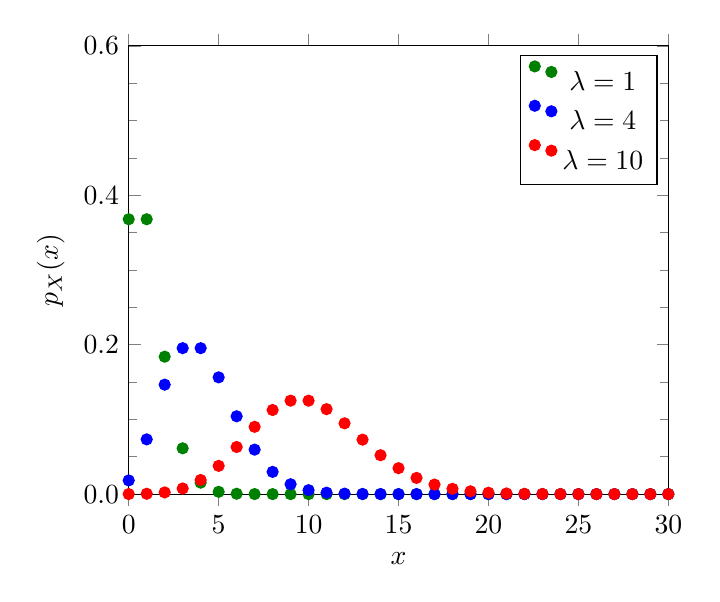
\begin{tikzpicture}[
                declare function={
                    poiss(\k,\lambda) = ((e^(-\lambda)*((\lambda^\k)/(\k!))));
                }
            ]
                \begin{axis}[
                    ybar,
                    xmin = 0, xmax = 30,
                    ymin = 0, ymax = 0.6,
                    minor y tick num = 3,
                    xlabel = {$x$},
                    ylabel = {$p_X(x)$},
                    samples at={0,...,30},
                    yticklabel style={
                        /pgf/number format/fixed,
                        /pgf/number format/fixed zerofill,
                        /pgf/number format/precision=1
                    }
                    ]

                    \addplot [only marks, Green] {poiss(x,1)}; \addlegendentry{$\lambda = 1$}
                    \addplot [only marks, blue] {poiss(x,4)}; \addlegendentry{$\lambda = 4$}
                    \addplot [only marks, red] {poiss(x,10)}; \addlegendentry{$\lambda = 10$}
                \end{axis}
            \end{tikzpicture}
        }

        \caption{Funzioni di massa di tre distribuzioni di Poisson.}
    \end{figure}

    \section{Proprietà delle distribuzioni discrete note}

    \subsection{Proprietà di perdita della memoria}

    Dopo aver visto le principali distribuzioni discrete, vediamo alcune loro proprietà. Partiamo da quella che viene detta \textbf{perdita di memoria}.
    
    Consideriamo il lancio di un dado a 6 facce. Vogliamo calcolare la probabilità che il numero di lanci richiesti prima di ottenere un 6 sia maggiore di 3. Osserviamo che questo problema è facilmente modellabile tramite una variabile aleatoria $X$ che descrive il numero di lanci effettuati. Inoltre, osserviamo che tale v.a. $X$ corrisponda ad una distribuzione geometrica in quanto descrive il numero di esiti richiesti per raggiungere un esito positivo (ossia ottenere un 6) in un processo di Bernoulli con infiniti esiti indipendenti tra loro. In particolare, abbiamo che $X \sim \mathrm{Geom}\rbk{\frac{1}{6}}$.

    Per calcolare $\Pr[X > 3]$ come richiesto dal problema, effettuiamo un passaggio al complemento:
    \[\begin{split}
        \Pr[X > 3] &= 1 - \Pr[X \leq 3] \\
        &= 1 - \sum_{i = 1}^{3} \Pr[X = i] \\
        &= 1 - \sum_{i = 1}^{3} \rbk{1-\frac{1}{6}}^{i-1} \frac{1}{6} \\
        &= \frac{125}{216} \\
    \end{split}\]

    In alternativa, osserviamo che è possibile calcolare più semplicemente tale probabilità:
    \[\Pr[X > 3] = \Pr[\text{i primi tre lanci falliscono}] = \rbk{1-\frac{1}{6}}^3 = \frac{125}{216}\]

    Supponiamo ora di aver già effettuato almeno 5 lanci e di voler calcolare la probabilità che ne siano richiesti altri 3, cioè la probabilità dell'evento $\{X > 3+5 \mid X > 5\}$. Utilizzando la definizione di probabilità condizionata, osserviamo che:
    \[\begin{split}
        \Pr[X > 8 \mid X > 5] &= \frac{\Pr[X > 8 \cap X > 5]}{\Pr[X > 5]} \\
        &= \frac{\Pr[X > 8]}{\Pr[X > 5]} \\
        &= \frac{\rbk{1-\frac{1}{6}}^8}{\rbk{1-\frac{1}{6}}^5} \\
        &= \frac{125}{216} \\
    \end{split}\]

    Concludiamo quindi che $ \Pr[X > 3+5 \mid X > 5] = \Pr[X > 3]$. Ciò non risulta essere un caso: essendo tutti i lanci indipendenti tra loro, il numero di lanci da attendere a partire dal sesto lancio è esattamente lo stesso del numero di lanci da attendere a partire dall'inizio, poiché nessuna informazione in più è giunta sul dado dai lanci precedenti. In questo senso, la distribuzione \curlyquotes{dimentica} quello che è accaduto in passato, dando il nome alla proprietà.
    
    Dimostreremo che tale proprietà di mancanza di memoria vale per qualsiasi coppia di valori nel caso delle distribuzioni geometriche. Più importamente, dimostreremo anche che le distribuzioni geometriche siano \underline{le uniche} distribuzioni discrete a godere di tale proprietà. In altre parole, se una variabile aleatoria discreta rispetta la proprietà allora essa deve obbligatoriamente seguire una distribuzione geometrica.

    \begin{framedthm}{Perdita di memoria della dist. geometrica}
        Data una v.a. discreta $X$ con $X(\Omega) = \N$, allora:
        \[\Pr[X > t + s \mid X > s ] = \Pr[X > t] \]
        vale per ogni $t,s \in \N$ se e solo se $X \sim \mathrm{Geom}(p)$ per qualche $p \in [0,1] \subset \R$.
    \end{framedthm}

    \begin{proof}
        Dimostriamo prima l'implicazione da destra a sinistra. Supponiamo che $X \sim \mathrm{Geom}(p)$ per qualche $p \in [0,1] \subset \R$. Fissati due valori $t,s \in \N$, procediamo analogamente all'esempio precedente:
        \[\begin{split}
            \Pr[X > t+s \mid X > s] &= \frac{\Pr[X > t+s \cap X > s]}{\Pr[X > s]} \\
            &= \frac{\Pr[X > t+s]}{\Pr[X > s]} \\
            &= \frac{(1-p)^{t+s}}{(1-p)^s} \\
            &= (1-p)^t \\
            &= \Pr[X > t] \\
        \end{split}\]

        concludendo che ogni v.a. a distribuzione geometrica goda della proprietà di perdita di memoria. Vediamo ora l'implicazione da sinistra a destra. Supponiamo di avere una v.a. $Y$ (non sappiamo la sua distribuzione) che gode della proprietà di perdita di memoria.

        \textbf{Fatto}: per ogni $k \in \N$ vale che $\Pr[Y > k] = \Pr[Y > 1]^k$

        \begin{proof}[Dimostrazione del fatto]
            Procediamo per induzione su $k \in \N$. Quando $k = 0$, abbiamo banalmente che $\Pr[Y > 0] = 1$ poiché almeno un esito sarà sempre necessario per ottenere un successo. Per tanto, abbiamo che $\Pr[Y > 0] = 1 = \Pr[Y > 1]^0$. 

            Assumiamo ora che il fatto valga per un certo $k \in \N$ e dimostriamo che vale anche per $k+1$. Poiché $Y$ gode di perdita di memoria, abbiamo che:
            \[\Pr[Y > k+1] = \Pr[Y > k+1 \mid Y > 1] \Pr[Y > 1]= \Pr[Y > k] \Pr[Y > 1]\]

            Dunque, utilizzando l'ipotesi induttiva otteniamo che:
            \[\Pr[Y > k+1] = \Pr[Y > k] \Pr[Y > 1] = \Pr[Y > 1]^k \Pr[Y > 1] = \Pr[Y > 1]^{k+1}\]
        \end{proof}

        Una volta dimostrato il fatto, osserviamo che:
        \[\begin{split}
            \Pr[Y = y] &= \Pr[Y > y-1] - \Pr[Y > y] \\
            &= \Pr[Y > 1]^{y-1} - \Pr[Y > 1]^y \\
            &= \Pr[Y > 1]^{y-1} (1- \Pr[Y > 1])
        \end{split}\]

        Ponendo $p' = 1-Pr[Y > 1]$, otteniamo che $\Pr[Y = y] = (1-p')^{y-1}p'$, concludendo che $Y \sim \mathrm{Geom}(p')$.
    \end{proof}

    \subsection{Somme tra distribuzioni simili indipendenti}

    In molte situazioni comuni, potremmo ritrovarci a dover sommare due variabili aleatorie indipendenti con distribuzione simile. In molti casi, la somma tra variabili indipendenti con distribuzione simile assume una distribuzione nota. 
    
    Ad esempio, potremmo essere interessati al numero totale di lanci con esito testa ottenuti in due sequenze di lanci (con quantitativo di lanci potenzialmente diversi) utilizzando la stessa moneta, cioè la somma $X+Y$ delle variabili $X \sim \mathrm{Bin}(n,p)$ e $Y \sim \mathrm{Bin}(m,p)$. Intuitivamente, si ha che $X + Y \sim \mathrm{Bin}(n+m, p)$, cioè $X+Y$ rappresenta il numero di successi su $n+m$ esiti con probabilità $p$ di successo.

    \begin{framedprop}{Somma tra due binomiali indipendenti}
        Date due v.a. $X \sim \mathrm{Bin}(n,p)$ e $Y \sim \mathrm{Bin}(m,p)$ indipendenti tra loro, si ha che $X + Y \sim \mathrm{Bin}(n+m, p)$
    \end{framedprop}

    \begin{proof}
        Siano $X_1, \ldots, X_n \sim \mathcal{B}(p)$ e $Y_1, \ldots, Y_m \sim \mathcal{B}(p)$ i due processi di Bernoulli che descrivono $X$ e $Y$, ossia $X = X_1 + \ldots + X_n$ e $Y = Y_1 + \ldots + Y_m$. Abbiamo quindi che $X+Y = X_1 + \ldots X_n + Y_1 +\ldots + Y_m$.
        
        Poiché $X$ e $Y$ sono indipendenti tra loro, per ogni coppia di indici $i,j$ si ha che $X_i$ e $Y_i$ sono indipendenti tra loro (altrimenti vi sarebbe almeno un evento dipendente per le due variabili). Dunque, $X+Y$ risulta descritta da un processo di Bernoulli $X_1, \ldots, X_n, Y_1, \ldots, Y_n \sim \mathcal{B}(p)$, concludendo che $X+Y \sim \mathrm{Bin}(n+m, p)$.
    \end{proof}

    Poiché la distribuzione di Poisson non è altro che una binomiale con un numero tendente ad infinito di esiti e una probabilità tendente a zero di successi, risulta intuitivo che anche la somma di due Poissoniane indipendenti dia luce ad una nuova Poissoniana ottenuta sommando i due parametri delle distribuzioni iniziali.

    \begin{framedprop}{Somma tra due Poissoniane indipendenti}
        Date due v.a. $X \sim \mathrm{Poiss}(\lambda)$ e $Y \sim \mathrm{Poiss}(\gamma)$ indipendenti tra loro, si ha che $X + Y \sim \mathrm{Bin}(\lambda + \gamma)$
    \end{framedprop}
    
    \begin{proof}
        Applicando la probabilità totale e l'indipendenza tra le due variabili osserviamo che:
        \[\begin{split}
            \Pr[X + Y = k] &= \sum_{i = 0}^{k} \Pr[X+Y = k \mid X = i] \Pr[X = i] \\
            &= \sum_{i = 0}^{k} \Pr[Y = k-i \mid X = i] \Pr[X = i] \\
            &= \sum_{i = 0}^{k} \Pr[Y = k-i] \Pr[X = i] \\
        \end{split}\]

        A questo punto, sostituiamo le due densità discrete con la loro forma estesa:
        \[\begin{split}
            \Pr[X+Y = k] &= \sum_{i = 0}^{k} e^{-\gamma} \frac{\gamma^{k-i}}{(k-i)!} \cdot e^{-\lambda} \frac{\lambda^{k}}{i!} \\
            &= e^{-(\lambda+\gamma)} \sum_{i = 1}^{k} \frac{\gamma^{k-i}}{(k-i)!} \frac{\lambda^{i}}{i!} \\
            &= e^{-(\lambda+\gamma)} \sum_{i = 1}^{k} \frac{\gamma^{k-i}}{(k-i)!} \frac{\lambda^{i}}{i!} \frac{k!}{k!} \\
            &= \frac{e^{-(\lambda+\gamma)}}{k!} \sum_{i = 1}^{k} \binom{k}{i} \gamma^{k-i} \lambda^i \\
        \end{split}\]

        Per la formula del binomio di Newton, concludiamo che:
        \[\Pr[X+Y = k] = \frac{e^{-(\lambda+\gamma)}}{k!} \sum_{i = 1}^{k} \binom{k}{i} \gamma^{k-i} \lambda^i = \frac{e^{-(\lambda+\gamma)}}{k!}(\lambda+\gamma)^k\]

        Per tanto, abbiamo che $X+Y \sim \mathrm{Poiss}(\lambda+\gamma)$.
    \end{proof}

    \newpage

    \subsection{Tempi di $n$-esimo successo}

    In molti casi, la somma tra due variabili indipendenti di distribuzione identica va a generare una nuova distribuzione completamente diversa. Ad esempio, è il caso della somma tra variabili geometriche.

    \begin{framedprop}{Somma tra due geometriche indipendenti}
        Date due v.a. $X \sim \mathrm{Geom}(p)$ e $Y \sim \mathrm{Geom}(p)$ indipendenti tra loro, si ha che:
        \[\Pr[X+Y = k] = (k-1)(1-p)^{k-2}p^2\]
    \end{framedprop}

    \begin{proof}
        Applicando la probabilità totale e l'indipendenza tra le due variabili osserviamo che:
        \[\begin{split}
            \Pr[X + Y = k] &= \sum_{i = 1}^{k-1} \Pr[X+Y = k \mid X = i] \Pr[X = i] \\
            &= \sum_{i = 1}^{k-1} \Pr[Y = k-i \mid X = i] \Pr[X = i] \\
            &= \sum_{i = 1}^{k-1} \Pr[Y = k-i] \Pr[X = i] \\
        \end{split}\]

        A questo punto, sostituiamo le due densità discrete con la loro forma estesa:
        \[\begin{split}
            \Pr[X+Y = k] &= \sum_{i = 1}^{k-1} (1-p)^{k-i-1}p \cdot (1-p)^{i-1}p \\
            &= \sum_{i = 1}^{k-1} (1-p)^{k-2} p^2 \\
            &= (1-p)^{k-2}p^2 \sum_{i = 1}^{k-1} 1 \\
            &= (k-1)(1-p)^{k-2}p^2
        \end{split}\]
    \end{proof}

    Intuitivamente, la somma $X+Y$ di due v.a. geometriche $X \sim \mathrm{Geom}(p)$ e $Y \sim \mathrm{Geom}(p)$ indipendenti corrisponde al numero di tentativi necessari per ottenere due esiti positivi. Formalmente diremmo che la somma $X+Y$ è un \textit{tempo di secondo successo}.
    
    Date $n$ v.a. $\Delta_1, \ldots, \Delta_n \sim \mathrm{Geom}(p)$ indipendenti, definiamo il \textbf{tempo di $n$-esimo successo} come la variabile aleatoria $T_n = \Delta_1, \ldots, \Delta_n$. Dimostriamo quindi che il tempo di $n$-esimo successo segue una distribuzione ben precisa, estendendo il lemma precedente.

    \begin{framedprop}{}
        Dato un tempo di $n$-esimo successo $T_n$, si ha che:
        \[\Pr[T_n = k] = \binom{k-1}{n-1} (1-p)^{k-n} p^n\]
    \end{framedprop}

    \begin{proof}
        Siano $\Delta_1, \ldots, \Delta_n \sim \mathrm{Geom}(p)$ le v.a. che descrivono $T_n$. Ssserviamo che $T_n$ può essere induttivamente definita come segue:
        \begin{itemize}
            \item $T_1 = \Delta_i$
            \item $T_i = T_{i-1} + \Delta_i$ per ogni $i > 1$
        \end{itemize}

        Procediamo quindi per induzione su $n$. Quando $n = 1$, abbiamo banalmente che:
        \[\Pr[T_n = k] = \Pr[\Delta_1 = k] = (1-p)^{k-1} p^1 = \binom{k-1}{0} (1-p)^{k-1} p^1\]

        Assumiamo quindi che la proposizione valga per un certo $n$ e dimostriamo che vale anche per $n+1$. Osserviamo che $T_{n}$ e $\Delta_{n+1}$ sono indipendenti tra loro poiché $\Delta_{n+1}$ è indipendente da $\Delta_1, \ldots, \Delta_{n}$. Per tanto, applicando la probabilità totale e l'indipendenza tra le due variabili osserviamo che:
        \[\begin{split}
            \Pr[T_{n+1} = k] &= \Pr[T_{n} + \Delta_{n} =k]\\
            &= \sum_{i = n}^{k-1} \Pr[T_{n} + \Delta_{n} = k \mid T_n = i] \Pr[\Delta_n = i] \\
            &= \sum_{i = n}^{k-1} \Pr[\Delta_n = k-i \mid T_n = i] \Pr[\Delta_n = i] \\
            &= \sum_{i = n}^{k-1} \Pr[\Delta_n = k-i] \Pr[T_n = i] \\
        \end{split}\]

        Applicando l'ipotesi induttiva, abbiamo che:
        \[\begin{split}
            \Pr[T_{n+1} = k] &= \sum_{i = n}^{k-1} (1-p)^{k-i-1}p \cdot \binom{i-1}{n-1} (1-p)^{i-n} p^n \\
            &= \sum_{i = n}^{k-1} (1-p)^{k-(n+1)} p^{n+1} \binom{i-1}{n-1} \\
            &= (1-p)^{k-(n+1)} p^{n+1} \sum_{i = n}^{k-1} \binom{i-1}{n-1} \\
        \end{split}\]

        Ora, utilizziamo un'identità nota del triangolo di Pascal (facilmente dimostrabile per induzione su $k$):
        \[\sum_{i = n}^{k-1} \binom{i-1}{n-1} = \binom{k-1}{n}\]

        concludendo il passo induttivo:
        \[\begin{split}
            \Pr[T_{n+1} = k] &= (1-p)^{k-(n+1)} p^{n+1} \sum_{i = n}^{k-1} \binom{i-1}{n-1} \\
            &= \binom{k-1}{(n+1)-1} (1-p)^{k-(n+1)} p^{n+1} \\
        \end{split}\]
    \end{proof}
    
    La distribuzione che descrive il tempo di $n$-esimo successo viene comunemente detta \textbf{distribuzione di Pascal}.
    
    \begin{frameddefn}{Distribuzione di Pascal}
        Una v.a. $X$ è detta a distribuzione di Pascal di parametri $n$ e $p$, indicato con $X \sim \mathrm{Pasc}(n,p)$, quando $X$ descrive il tempo di $n$-esimo successo con probabilità di successo $p$.

        Per ogni v.a $X \sim \mathrm{Pasc}(n,p)$ vale che:
        \begin{itemize}
            \item $X(\Omega) = \N$ con $n > 0$ e $p \in [0,1] \subset \R$
            \item La funzione di massa è dettata da:
            \[p_X(k) = \binom{k-1}{n-1} (1-p)^{k-n} p^n\]
            per $n \leq k$, altrimenti 0.
        \end{itemize}
    \end{frameddefn}
    
    \begin{figure}[H]
        \centering
        \resizebox{0.6\textwidth}{!}{
            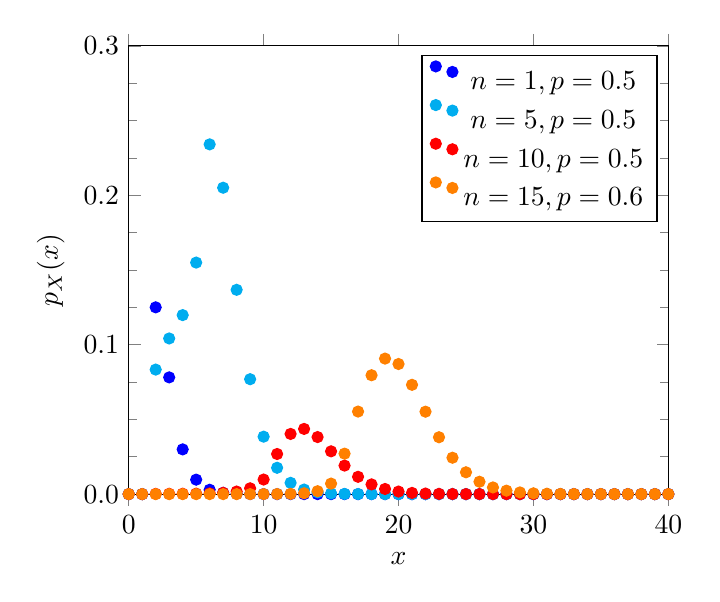
\begin{tikzpicture}[
                declare function={pascal(\k,\n,\p)=(\k!-1)/((\n-1)!*(\k-\n)!)*(1-\p)^(\k-\n)*(\p)^(\k);}
            ]
                \begin{axis}[
                    ybar,
                    xmin = 0, xmax = 40,
                    ymin = 0, ymax = 0.3,
                    minor y tick num = 3,
                    xlabel = {$x$},
                    ylabel = {$p_X(x)$},
                    samples at={0,...,100},
                    yticklabel style={
                        /pgf/number format/fixed,
                        /pgf/number format/fixed zerofill,
                        /pgf/number format/precision=1
                    }
                    ]

                    \addplot [only marks, blue, domain = 1:50] {pascal(x,1,0.5)}; \addlegendentry{$n = 1, p=0.5$}
                    \addplot [only marks, cyan, domain = 5:50] {pascal(x,5,0.5)}; \addlegendentry{$n = 5, p=0.5$}
                    \addplot [only marks, red, domain = 10:50] {pascal(x,10,0.5)}; \addlegendentry{$n = 10, p=0.5$}
                    \addplot [only marks, orange, domain = 15:50] {pascal(x,15,0.6)}; \addlegendentry{$n = 15, p=0.6$}
                \end{axis}
            \end{tikzpicture}
        }

        \caption{Funzioni di massa di quattro distribuzioni di Pascal.}
    \end{figure}
    

    \chapter{Valore atteso, Varianza e Covarianza}

    \section{Valore atteso}

    \subsection{Intuizione e definizione}

    Consideriamo il lancio di un classico dado a sei facce. Ci chiediamo quale sia in media il valore che ci aspettiamo come risultato del lancio. Decidiamo di calcolare tale valore come la media di tutti i risultati possibili, dunque:
    \[\frac{1+2+3+4+5+6}{6} = \frac{21}{6} = 3.5\]

    concludendo che il valore medio del lancio sia $3.5$. Immaginiamo ora di avere un dado modificato, dove la faccia 4 è stata sostituita con un'altra faccia 3 e la faccia 5 è stata sostituita con un'altra faccia 2. In tal caso, il valore medio dei possibili risultati risulta essere:
    \[\frac{1+2+3+3+2+6}{6} = \frac{21}{6} = 3.5\]

    Manipolando algebricamente il conto ottenuto, abbiamo che:
    \[\frac{1+2+3+3+2+6}{6} = \frac{1+2 \cdot 2 + 3 \cdot 2 + 6}{6} = 1 \cdot \frac{1}{6} + 2 \cdot \frac{2}{6} + 3 \cdot \frac{2}{6} + 4 \cdot \frac{1}{6} + 6 \cdot \frac{1}{6}\]

    Ponendo $X$ come la v.a. che descrive il lancio di tale dado modificato, osserviamo che:
    \[1 \cdot \frac{1}{6} + 2 \cdot \frac{2}{6} + 3 \cdot \frac{2}{6} + 4 \cdot \frac{1}{6} + 6 \cdot \frac{1}{6} = 1 \cdot p_X(1) + 2 \cdot p_X(2) + 3 \cdot p_X(3) + 4 \cdot p_X(4) + 6 \cdot p_X(6)\]

    tale somma di tutti i prodotti tra i valori possibili di $X$ e le probabilità che tali valori si verifichino viene detta \textbf{valore atteso} di $X$, tipicamente indicato come $\Exp[X]$.

    \begin{frameddefn}{Valore atteso (v.a. discrete)}
        Data una v.a. discreta $X$, definiamo il valore atteso di $X$, indicato con $\Exp[X]$, come:
        \[\Exp[X] = \sum\limits_{x \in X(\Omega)} x \Pr[X = x]\]
    \end{frameddefn}

    Oltre a rappresentare una sorta di \curlyquotes{media pesata dalla probabilità}, il valore atteso ha anche molte applicazioni pratiche dalle più banali alle più avanzate.
    
    Immaginiamo di star camminando per strada. Un signore dall'aspetto losco ci propone di giocare al suo semplice gioco a premi: lanciando un dado a 6 facce, se il risultato corrisponde a 6 allora il giocatore vince 30€, altrimenti non vince nulla. La quota di partecipazione al gioco è di 10€.

    Prima di scegliere se giocare o no, ci chiediamo se il gioco valga effettivamente la candela (ossia se il guadagno medio che ci aspettiamo sia positivo o negativo). Modelliamo quindi la variabile aleatoria $X$ descrivente il guadagno derivato dal gioco. Poiché la quota fissa è 10€ abbiamo che $X(\Omega) = \{-10, 20\}$, ottenendo quindi che:
    \[\Exp[X] = 20 \Pr[X = 20] + (-10) \Pr[X = -10] = 20 \cdot \frac{1}{6} + (-10) \cdot \frac{5}{6} = -5\]

    Concludiamo quindi che il guadagno atteso dal gioco sia negativo e dunque che esso sia una truffa! Dopo aver inveito verso lo sconosciuto, quest'ultimo ci chiede scusa, rammaricato. Mentre decidiamo di andarcene per la nostra strada, il signore ci ferma nuovamente e ci chiede consiglio su quale potrebbe essere una giusta quota da chiedere in futuro, mantenendo le stesse regole del gioco (dunque una potenziale vincita di 30€ quando esce 6 dal lancio).
    
    Modelliamo quindi la domanda come un'altra variabile aleatoria $Y$ descrivente la vincita derivata dal gioco (dunque non considerando la quota pagata). Osserviamo come:
    \[\Exp[Y] = 30 \Pr[Y = 30] + 0 \Pr[Y = 0] = 30 \cdot \frac{1}{6} + 0 \cdot \frac{5}{6} = 5\]

    Poiché la vincita attesa è 5€, consigliamo al venditore di chiedere una quota di 5€, in modo che la vincita media corrisponda alla quota fissa.
    
    Questa non è altro che la definizione matematica di \textbf{gioco equo}, ossia un gioco in cui, a lungo termine, le probabilità di guadagno e perdita sono uguali per tutti i giocatori. In altre parole, un gioco è equo quando il risultato finale non favorisce né penalizza nessun partecipante in modo sistematico, e il vantaggio per ciascun giocatore deriva solo dalla fortuna o dalle abilità (a seconda del tipo di gioco), non da un meccanismo sbilanciato.
    
    Nel gioco d'azzardo, ad esempio, i casinò cercano di progettare giochi \textit{non equi} (come la roulette o il blackjack) a valore atteso negativo, in modo che il banco abbia una leggero guadagno atteso migliore rispetto a quello dei giocatori. Similmente, nel mercato azionario un piano di investimento è considerabile ottimo quando il valore atteso del guadagno è positivo.

    \subsection{Proprietà del valore atteso}

    Una fondamentale proprietà del valore atteso risulta essere la sua \textbf{linearità}, ossia la caratteristica per cui dati due valori $a,b \in \R$ si abbia che $\Exp[aX + Yb] = a \Exp[X]+b\Exp[Y]$, per ogni coppia $X,Y$ di variabili aleatorie. Questa proprietà permette di scomporre il calcolo del valore atteso di v.a. più complesse tramite la somma dei valori attesi di altre v.a. che lo descrivono.
    
    Ad esempio, riprendendo ancora il nostro problema relativo al lancio di due dadi con $X = X_1 + X_2$, concludiamo immediatamente che:
    \[\Exp[X] = \Exp[X_1 + X_2] = \Exp[X_1] + \Exp[X_2] = 2 \Exp[X_1]\] 

    poiché $X_1$ e $X_2$ sono due v.a. con densità identica.

    Prima di procedere, osserviamo che ogni valore atteso possa essere riscritto come una somma che si estende per tutto lo spazio ambiente, invece che solo sull'immagine della variabile aleatoria. Questa riformulazione ci permette di trattare facilmente le interazioni tra variabili aleatorie.

    \begin{framedlem}{}
        Data una v.a. discreta $X$, si ha che:
        \[\Exp[X] = \sum_{\omega \in \Omega} X(\omega) \Pr[\{\omega\}] \]
    \end{framedlem}

    \begin{proof}
        Per definizione stessa, abbiamo che:
        \[\Exp[X] = \sum_{x \in X(\Omega)} x \Pr[X = x] = \sum_{x \in X(\Omega)} x \rbk{\sum_{\substack{\omega \in \Omega \,: \\X(\omega) = x}} \Pr[\{\omega\}]}\]

        Portando $x$ all'interno della seconda sommatoria e sfruttando il fatto che in essa valga $X(\omega) = x$, otteniamo che:
        \[\begin{split}
            \Exp[X] &= \sum_{x \in X(\Omega)} \sum_{\substack{\omega \in \Omega \,: \\X(\omega) = x}} x \Pr[\{\omega\}] \\
            &= \sum_{x \in X(\Omega)} \sum_{\substack{\omega \in \Omega \,: \\X(\omega) = x}} X(\omega) \Pr[\{\omega\}] \\
            &=\sum_{\omega \in \Omega} X(\omega) \Pr[\{\omega\}]
        \end{split}\]
    \end{proof}

    \begin{framedthm}{Linearità del valore atteso}
        Date due v.a. discrete $X, Y$ e due valori $\alpha,\beta \in \R$, si ha che:
        \[\Exp[\alpha X+ \beta Y] = \alpha \Exp[X] + \beta\Exp[Y]\]
    \end{framedthm}

    \begin{proof}
        Per il lemma precedente abbiamo che:
        \[\Exp[\alpha X + \beta Y] = \sum_{\omega \in \Omega} (\alpha X + \beta Y)(\omega) \Pr[\{\omega\}]\]

        essendo $\alpha, \beta$ due costanti ed essndo $X$ e $Y$ due funzioni, abbiamo che $(\alpha X + \beta Y)(\omega) = \alpha X(\omega) + \beta Y(\omega)$, dunque:
        \[\Exp[\alpha X + \beta Y] = \sum_{\omega \in \Omega} (\alpha X(\omega) + \beta Y(\omega)) \Pr[\{\omega\}]\]

        Infine, distribuendo $\Pr[\{\omega\}]$ concludiamo che:
        \[\begin{split}
            \Exp[\alpha X + \beta Y] &= \sum_{\omega \in \Omega} \alpha X(\omega) \Pr[\{\omega\}] + \beta Y(\omega) \Pr[\{\omega\}] \\
            &= \alpha \sum_{\omega \in \Omega}  X(\omega) \Pr[\{\omega\}] + \beta \sum_{\omega \in \Omega} Y(\omega) \Pr[\{\omega\}] \\
            &= \alpha \Exp[X] + \beta \Exp[Y]
        \end{split}\]
    \end{proof}

    Tramite la linearità è possibile ottenere numerose altre proprietà del valore atteso. La più banale, è la possibilità di estendere la linearità ad un insieme $X_1, \ldots, X_n$ di variabili aleatorie (facilmente dimostrabile per induzione, lo stesso vale per il caso continuo).
    \[\Exp \sbk{\sum_{i = 1}^n X_i} = \sum_{i = 1}^n \Exp[X_i]\]

    La seconda proprietà, invece, richiede essere più scaltri. Data una variabile aleatoria $X$ e due valori $\alpha, \beta \in \R$, si ha che $\Exp[\alpha X + \beta] = \alpha \Exp[X] + \beta$. Osserviamo che questa proprietà può essere derivata dalla linearità del valore atteso considerando una seconda variabile $Y$ che assume sempre e solo il valore $1$. Per tale variabile abbiamo chiaramente che $\Exp[Y] = 1$, dunque ne segue immediatamente che:
    \[\Exp[\alpha X + \beta Y] = \alpha \Exp[X] + \beta \Exp[Y] = \alpha \Exp[X] + \beta\]

    Un'altra proprietà fondamentale del valore atteso è la sua persistenza dei pesi probabilistici quando viene applicato ad una funzione definita su una variabile aleatoria. In generale, data una funzione $f$ ed una variabile aleatoria $X$, applicare $f$ ad $X$ corrisponde a comporre $f$ con $X$, dunque $f(X)(\omega) = f(X(\omega))$.
    
    La proprietà di persistenza è data dalla \textbf{legge dello statistico inconsapevole} (dall'inglese \textit{law of the unconscious statistician}), nome dovuto alla presunta tendenza a pensare alla suddetta legge come la definizione stessa del valore atteso di una funzione $g(X)$ e di una variabile casuale $X$, piuttosto che (più formalmente) come una conseguenza della vera definizione di valore atteso.

    \begin{framedthm}[label={inc_stat}]{Legge dello statistico inconsapevole}
        Data una v.a. discreta $X$ ed una funzione $f$, si ha che:
        \[\Exp[f(X)] = \sum_{x \in X(\Omega)} f(x) p_X(x)\]
    \end{framedthm}

    \begin{proof}
        Per definizione abbiamo che:
        \[\Exp[f(X)] = \sum_{z \in f(X(\Omega))} z \Pr[f(X) = z] = \sum_{z \in f(X(\Omega))} z \sum_{\substack{x \in X(\Omega) \\ f(x) = z}} \Pr[X = x]\]

        Portando $z$ all'interno della seconda sommatoria e sfruttando il fatto che in essa valga $f(x) = z$, otteniamo che:
        \[\begin{split}
            \Exp[f(X)] &= \sum_{z \in f(X(\Omega))} \sum_{\substack{x \in X(\Omega) \\ f(x) = z}} z \Pr[X = x] \\
            &= \sum_{z \in f(X(\Omega))} \sum_{\substack{x \in X(\Omega) \\ f(x) = z}} f(x) \Pr[X = x] \\
            &= \sum_{x \in X(\Omega)} f(x) \Pr[X = x] \\
        \end{split}\]
    \end{proof}

    Tramite la legge appena dimostrata, è possibile dimostrare che il valore atteso sia un operatore \textit{idempotente}, ossia che componendolo con se stesso otteniamo la funzione originale. In altre parole, si ha che $\Exp[\Exp[X]] = \Exp[X]$. Tra tutte le proprietà viste fin'ora, questa risulta decisamente come la più intuitiva: la media della media è uguale alla media!

    \begin{framedprop}{Idempotenza del valore atteso}
        Data una v.a. discreta, si ha che $\Exp[\Exp[X]] = \Exp[X]$
    \end{framedprop}

    \begin{proof}
        Dimostriamo la proposizione solo per il caso discreto. Per il teorema precedente abbiamo che: 
        \[\Exp[\Exp[X]] =  \sum_{x \in X(\Omega)} \Exp[x] \Pr[X = x] = \sum_{x \in X(\Omega)} x \Pr[X = x] = \Exp[X]\]
    \end{proof}

    Un'altra proprietà elementare del valore atteso è la sua monotonia: se due variabili aleatorie $X$ ed $Y$ sono tali che $X(\omega) \geq Y(\omega)$ per ogni $\omega \in \Omega$, abbreviato in $X \geq Y$, allora $\Exp[X] \geq \Exp[Y]$.

    \begin{framedthm}{Monotonia del valore atteso}
        Date due v.a. discrete $X$ e $Y$, se $X \geq Y$ allora $\Exp[X] \geq \Exp[Y]$
    \end{framedthm}

    \begin{proof}
        Assunto $X \geq Y$, sia $Z$ la v.a. definita come $Z = X - Y$. Poiché $X \geq Y$, sappiamo che $Z \geq 0$. Per tanto, deve valere che $\Exp[Z] \geq 0$. Dalla linearità del valore atteso otteniamo quindi che:
        \[0 \leq \Exp[Z] = \Exp[X-Y] = \Exp[X] - \Exp[Y]\]
        Concludiamo dunque che $\Exp[X] \geq \Exp[Y]$. 
    \end{proof}

    Nella sua forma più semplice, cioè con $\alpha, \beta = 1$, la linearità del valore atteso afferma che $\Exp[X + Y] = \Exp[X] + \Exp[Y]$, ossia che il valore atteso della somma di due v.a. è uguale alla somma dei valori attesi delle due v.a. stesse. Risulta naturale quindi chiedersi se lo stesso valga anche per il prodotto tra due v.a., ossia se $\Exp[XY] = \Exp[X] \Exp[Y]$. In questo caso, la risposta alla domanda è \underline{non sempre}.

    Prima di tutto, osserviamo che due qualsiasi v.a. vale che:
    \[\begin{split}
        \Exp[XY] &= \sum_{z \in XY(\Omega)} z \Pr[XY = z] \\
        &= \sum_{z \in XY(\Omega)} z \sum_{x \in X(\Omega)} \Pr\sbk{X = x, Y = \frac{z}{x}} \\
        &= \sum_{x \in X(\Omega)} \sum_{z \in XY(\Omega)} z \Pr\sbk{X = x, Y = \frac{z}{x}} \\
        &= \sum_{x \in X(\Omega)} \sum_{y \in Y(\Omega)} xy \Pr[X = x, Y = y] \\
    \end{split}\]

    Per concludere la dimostrazione, ci basterebbe spezzare la probabilità $\Pr[X = x, Y = y]$ nel prodotto $\Pr[X = x] \Pr[Y = y]$. Tuttavia, ciò è possibile se e solo se le due variabili aleatorie sono indipendenti.
    \label{ind_exp_val}

    \begin{framedthm}{}
        Date due v.a. discrete $X$ ed $Y$, se le due variabili sono indipendenti tra loro allora $\Exp[XY] = \Exp[X]\Exp[Y]$.
    \end{framedthm}

    \begin{proof}
        Assumendo che $X$ ed $Y$ siano indipendenti, dall'osservazione precedente concludiamo immediatamente che:
        \[\begin{split}
            \Exp[XY] &=  \sum_{x \in X(\Omega)} \sum_{y \in Y(\Omega)} xy \Pr[X = x, Y = y] \\
            &= \sum_{x \in X(\Omega)} \sum_{y \in Y(\Omega)} xy \Pr[X = x]\Pr[Y = y] \\
            &= \sum_{x \in X(\Omega)} x \Pr[X = x] \sum_{y \in Y(\Omega)} y\Pr[Y = y] \\
            &= \sum_{x \in X(\Omega)} x \Pr[X = x] \Exp[Y] \\
            &= \Exp[Y] \sum_{x \in X(\Omega)} x \Pr[X = x] \\
            &= \Exp[Y] \Exp[X] \\
        \end{split}\]
    \end{proof}

    Cosa accade invece se le due variabili aleatorie sono \textit{dipendenti}? È sempre vero che il valore atteso del loro prodotto è \textit{diverso} dal prodotto dei loro valori attesi? Consideriamo ad esempio due v.a. $X, Y$ tali che $Y = X^2$, dove $X(\Omega) = \{-1,0,1\}$ e:
    \[\Pr[X = -1] = \frac{1}{5} \qquad \Pr[X = 0] = \frac{3}{5} \qquad \Pr[X = 1] = \frac{1}{5}\]

    Per definizione stessa risulta chiaro che $X$ ed $Y$ siano dipendenti tra loro. Difatti, abbiamo che:
    \[\Pr[X = -1, Y = 0] = 0 \neq \frac{3}{25} = \Pr[X = -1] \Pr[Y = 0]\]

    Usando la legge dello stocastico inconsapevole, calcoliamo facilmente i tre valori attesi di nostro interesse:
    \[\Exp[X] = (-1) \cdot \frac{1}{5} + 0 \cdot \frac{3}{5} + 1 \cdot \frac{1}{5} = 0\]
    \[\Exp[Y] = \Exp[X^2] = (-1)^2 \cdot \frac{1}{5} + 0^2 \cdot \frac{3}{5} + 1^2 \cdot \frac{1}{5} = \frac{2}{5}\]
    \[\Exp[XY] = \Exp[X^3] = \Exp[X^2] = (-1)^3 \cdot \frac{1}{5} + 0^3 \cdot \frac{3}{5} + 1^3 \cdot \frac{1}{5} = 0\]

    concludendo quindi che $\Exp[XY] = 0 = \Exp[X] \Exp[Y]$ nonostante $X$ ed $Y$ siano dipendenti tra loro.

    \begin{framedobs}{}
        Date due v.a. $X$ e $Y$ dipendenti tra loro, non è detto che $\Exp[XY] \neq \Exp[X] \Exp[Y]$
    \end{framedobs}

    Come mostrato nella \Cref{va_cong_cond_marg}, è possibile che il condizionamento di variabili aleatorie su un evento noto generi una seconda variabile aleatoria. In particolare, nell'esempio discusso abbiamo visto come $(Y \mid X = x) \sim \mathrm{Bin}\rbk{x, \frac{1}{6}}$. In generale, quindi, dato un evento $A$ indichiamo con $X \mid A$ la variabile aleatoria ottenuta post-condizionamento.

    \begin{framedprop}{}
        Data una v.a. discreta $X$ ed un evento $A$ si ha che:
        \[\Exp[X \mid A] = \frac{\Exp[X \cdot \1_A]}{\Pr[A]}\]
        Inoltre, se $\{X = x\}$ e $A$ sono indipendenti per ogni $x \in \Omega(A)$ allora:
        \[\Exp[X \mid A] = \Exp[X]\]
    \end{framedprop}

    \begin{proof}
        Applicando la definizione di probabilità condizionata abbiamo che:
        \[\Exp[X \mid A] = \sum_{x \in X(\Omega)} x \Pr[X = x \mid A] = \sum_{x \in X(\Omega)} x \frac{\Pr[X = x], A}{\Pr[A]} = \frac{\Exp[X \cdot \1_A]}{\Pr[A]}\]

        Similmente, applicando l'indipendenza abbiamo che:
        \[\Exp[X \mid A] = \sum_{x \in X(\Omega)} x \Pr[X = x \mid A] = \sum_{x \in X(\Omega)} x \Pr[X = x] = \Exp[X]\]
    \end{proof}

    Il valore atteso condizionato può essere utilizzato anche per calcolare un \curlyquotes{valore atteso totale}, cioè l'equivalente per il valore atteso della probabilità totale.

    \begin{framedprop}{Valore atteso totale }
        Sia $X$ una v.a. discreta. Data una partizione $A_1, \ldots, A_n$ di $\Omega$ si ha che:
        \[\Exp[X] = \sum_{i = 1}^n \Exp[X \mid A_i] \cdot \Pr[A_i]\]
    \end{framedprop}
    
    \begin{proof}
        Utilizzando la probabilità totale abbiamo che:
        \[\begin{split}
            \Exp[X] &= \sum_{x \in X(\Omega)} x \Pr[X = x] \\
            &= \sum_{x \in X(\Omega)} x \sum_{i = 1}^n \Pr[X = x \mid A_i] \Pr[A_i] \\
            &= \sum_{i = 1}^n  \Pr[A_i] \sum_{x \in X(\Omega)} x \Pr[X = x \mid A_i]  \\
            &= \sum_{i = 1}^n  \Pr[A_i] \Exp[X \mid A_i]  \\
        \end{split}\]
    \end{proof}

    Supponiamo ora di avere due variabili aleatorie $X$ e $Y$ e di essere interessati a conoscere il valore atteso del valore atteso su tutti i condizionamenti possibili su $Y$ dati da $X$. Formalmente, ciò corrisponde al valore atteso $\Exp[f(x)]$ dove $f(x) = \Exp[Y \mid X = x]$. Per brevità, scriveremo $\Exp[Y \mid X]$ per indicare la funzione su variabile aleatoria $f(X)$. Il valore $\Exp[\Exp[Y \mid X]]$ rappresenta quindi, intuitivamente, la media tra tutte le medie ottenute dai condizionamenti, dando una visione di insieme.
    
    Non così sorprendentemente, questo valore coincide esattamente con $\Exp[Y]$. Difatti, $\Exp[\Exp[Y \mid X]]$ può essere visto come un \curlyquotes{valore atteso totale}. Questo ci permette quindi di calcolare $\Exp[Y]$ passando per i valori attesi condizionati $\Exp[Y \mid X = x]$, ovviamente nel caso in cui essi siano più facili da calcolare.

    \begin{framedthm}{}
        Date due v.a. discrete $X$ e $Y$ si ha che $\Exp[\Exp[Y \mid X]] = \Exp[Y]$.
    \end{framedthm}

    \begin{proof}
        Sia $f$ la funzione definita come $f(x) = \Exp[Y \mid X = x]$. Tramite il \Cref{inc_stat} e la proposizione precedente abbiamo che:
        \[\begin{split}
            \Exp[\Exp[Y \mid X]] &= \Exp[f(X)] \\
            &= \sum_{x \in X(\Omega)} f(x) \Pr[X = x] \\
            &= \sum_{x \in X(\Omega)} \Exp[Y \mid X = x] \Pr[X = x] \\
            &= \Exp[Y] \\
        \end{split}\]
    \end{proof}


    \subsection{Valore atteso di distribuzioni note}
    \label{exp_noti}

    Nel capitolo precedente abbiamo discusso come individuare la distribuzione del fenomeno aleatorio che vogliamo descrivere ci permetta di calcolare rapidamente le probabilità che lo riguardano. Per estensione, risulta naturale pensare che le distribuzioni più comuni abbiano dei valori attesi già noti.

    Consideriamo ad esempio una variabile di Bernoulli $X \sim \mathcal{B}(p)$. Osserviamo facilmente che:
    \[\Exp[X] = 0 \cdot \Pr[X = 0] + 1 \cdot \Pr[X = 1] = \Pr[X = 1] = p\]

    In altre parole, il valore medio assunto da un esito di Bernoulli è precisamente la probabilità che esso sia un esito positivo.

    \begin{framedprop}{Valore atteso di una Bernoulliana}
        Data una v.a. $X$ tale che $X \sim \mathcal{B}(p)$, si ha che:
        \[\Exp[X] = p\]
    \end{framedprop}

    Procedendo sulla stessa onda, dimostriamo i valori attesi di tutte le distribuzioni discrete introdotte.

    \begin{framedprop}{Valore atteso di una uniforme discreta}
        Data una v.a. $X$ tale che $X \sim \mathcal{U}\{a,b\}$, si ha che:
        \[\Exp[X] = \frac{a+b}{2}\]
    \end{framedprop}

    \begin{proof}
        Trattandosi di un'uniforme discreta abbiamo che:
        \[\begin{split}
            \Exp[X] &= \sum_{k =a}^b k \Pr[X = k]\sum_{k = a}^b k \frac{1}{b-(a-1)} \\
            &= \frac{1}{b-(a-1)} \rbk{\sum_{k = 1}^{b} k - \sum_{k}^{a-1} k} \\
            &= \frac{1}{b-a+1} \rbk{\frac{b(b+1)}{2} - \frac{(a-1)a}{2}}\\
            &= \frac{(a+b)(b-a+1)}{2(b-a+1)} \\
            &= \frac{a+b}{2}
        \end{split}\]
    \end{proof}
    
    \begin{framedprop}{Valore atteso di una binomiale}
        Data una v.a. $X$ tale che $X \sim \mathrm{Bin}(n,p)$, si ha che:
        \[\Exp[X] = np\]
    \end{framedprop}

    \begin{proof}
        Siano $X_1, \ldots, X_n \sim \mathcal{B}(p)$ le v.a. che definiscono il processo di Bernoulli descritto da $X$, dunque $X = X_1 + \ldots + X_n$. Tramite la linearità del valore atteso e la proposizione precedente, concludiamo immediatamente che:
        \[\Exp[X] = \Exp[X_1 + \ldots + X_n] = \Exp[X_1] + \ldots + \Exp[X_n] = np\]
    \end{proof}

    \begin{framedprop}{Valore atteso di una geometrica}
        Data una v.a. $X$ tale che $X \sim \mathrm{Geom}(p)$, si ha che:
        \[\Exp[X] = \frac{1}{p}\]
    \end{framedprop}

    \begin{proof}
        Trattandosi di una geometrica abbiamo che:
        \[\begin{split}
            \Exp[X] &= \sum_{k = 1}^{+\infty} k \Pr[X = k] = \sum_{k = 1}^{+\infty} k (1-p)^{k-1} p = p \sum_{k = 1}^{+\infty} k (1-p)^{k-1}\\
        \end{split}\]

        Osserviamo come ogni termine $k$-esimo della somma infinita corrisponda alla derivata in $p$ di $-(1-p)^k$. Per tanto, abbiamo che:
        \[\begin{split}
            \Exp[X] &= p\sum_{k = 1}^{+\infty} k (1-p)^{k-1}  = p\sum_{k = 1}^{+\infty} \frac{\diff}{\diff p} \rbk{- (1-p)^{k}} \\
        \end{split}\]

        dove $\frac{\diff}{\diff p}$ è l'operatore di derivata in $p$. Poiché una somma di derivate è uguale alla derivata della somma, otteniamo che:
        \[\begin{split}
            \Exp[X] &= p\sum_{k = 1}^{+\infty} \frac{\diff}{\diff p} (1-p)^{k}  = p \, \frac{\diff}{\diff p} \rbk{- \sum_{k = 1}^{+\infty} (1-p)^{k}}  \\
        \end{split}\]

        A questo punto, osserviamo che la somma ottenuta sia nota e corrisponde alla somma geometrica di ragione $q = 1-p$. Poiché $-1 < q < 1$, otteniamo che:
        \[\begin{split}
            \Exp[X] &= p \, \frac{\diff}{\diff p} \rbk{- \sum_{k = 1}^{+\infty} (1-p)^{k}} \\
            &= p \, \frac{\diff}{\diff p} \rbk{- \frac{1}{1-(1-p)}} \\
            &= p \, \frac{\diff}{\diff p} \rbk{- \frac{1}{p}} \\
            &= p \, \frac{1}{p^2} \\
            &= \frac{1}{p} \\
        \end{split}\]
    \end{proof}

    \begin{framedprop}{Valore atteso di una ipergeometrica}
        Data una v.a. $X$ tale che $X \sim \mathrm{Hyp}(N,K,n)$, si ha che:
        \[\Exp[X] = \frac{Kn}{N}\]
    \end{framedprop}

    \begin{proof}
        Trattandosi di una ipergeometrica abbiamo che:
        \[\begin{split}
            \Exp[X] &= \sum_{k = 0}^n k \Pr[X = k] = \sum_{k = 0}^n k \, \frac{\binom{K}{k} \binom{N-K}{n-k}}{\binom{N}{n}} \\
        \end{split}\]

        Osserviamo che il primo termine della sommatoria può essere rimosso in quanto contiene un prodotto con $k = 0$, ottenendo:
        \[\Exp[X] = \sum_{k = 1}^n k \, \frac{\binom{K}{k} \binom{N-K}{n-k}}{\binom{N}{n}}\]

        A questo punto, osserviamo che per qualsiasi coppia $i,j \in \N$ con $i \leq j$ vale che:
        \[\binom{i}{j} = \frac{i!}{j! (i-j)!} = \frac{i}{j} \frac{(i-1)!}{(j-1)! (i-1-(j-1))!} = \frac{i}{j} \binom{i-1}{j-1}\]

        Per tanto, si ha che:
        \[\begin{split}
            \Exp[X] &= \sum_{k = 1}^n k \, \frac{\binom{K}{k} \binom{N-K}{n-k}}{\binom{N}{n}} = \frac{nK}{N} \sum_{k = 1}^n \frac{\binom{K-1}{k-1} \binom{N-1-(K-1)}{n-1-(k-1)}}{\binom{N-1}{n-1}}\\
        \end{split}\]

        Poniamo quindi $j = k-1$ per riaggiustare gli indici della sommatoria:
        \[\begin{split}
            \Exp[X] &= \frac{nK}{N} \sum_{j = 0}^n \frac{\binom{K-1}{j} \binom{N-1-(K-1)}{n-1-j}}{\binom{N-1}{n-1}}\\
        \end{split}\]

        Notiamo quindi che la somma ottenuta corrisponde alla somma di tutte le probabilità di una variabile $Y \sim \mathrm{Hyp}(N-1, K-1, n-1)$, implicando che essa equivalga 1 e dunque che:
        \[\begin{split}
            \Exp[X] &= \frac{nK}{N}
        \end{split}\]
    \end{proof}


    \begin{framedprop}{Valore atteso di una Poissoniana}
        Data una v.a. $X$ tale che $X \sim \mathrm{Poiss}(\lambda)$, si ha che:
        \[\Exp[X] = \lambda\]
    \end{framedprop}
    
    \begin{proof}
        Trattandosi di una Poissoniana abbiamo che:
        \[\begin{split}
            \Exp[X] &= \sum_{k=0}^{\infty} k \Pr[X = k] = \sum_{k=0}^{\infty} k e^{-\lambda} \frac{\lambda^k}{k!} = e^{-\lambda} \lambda \sum_{k=0}^{\infty} k  \frac{\lambda^{k-1}}{k!}
        \end{split}\]

        Osserviamo che il primo termine della sommatoria può essere rimosso in quanto contiene un prodotto con $k = 0$: 
        \[\begin{split}
            \Exp[X] &= e^{-\lambda} \lambda \sum_{k=1}^{\infty} k  \frac{\lambda^{k-1}}{k!} = e^{-\lambda} \lambda \sum_{k=1}^{\infty} \frac{\lambda^{k-1}}{(k-1)!} \\
        \end{split}\]

        Poniamo quindi $j = k-1$ per riaggiustare gli indici della sommatoria:
        \[\Exp[X] = e^{-\lambda} \lambda \sum_{j=0}^{\infty} \frac{\lambda^{j}}{j!}\]
        
        Notiamo quindi che la somma ottenuta corrisponda alla serie di Taylor di ordine infinito della funzione esponenziale, concludendo immediatamente che:
        \[ \Exp[X] = e^{-\lambda} \lambda \sum_{j=0}^{\infty} \frac{\lambda^{j}}{j!} = e^{-\lambda} \lambda e^{\lambda} = \lambda \]
    \end{proof}

    \begin{framedprop}{Valore atteso di una Pascaliana}
        Data una v.a. $X$ tale che $X \sim \mathrm{Pasc}(n,p)$, si ha che:
        \[\Exp[X] = \frac{n}{p}\]
    \end{framedprop}

    \begin{proof}
        Siano $\Delta_1, \ldots, \Delta_n \sim \mathrm{Geom}(p)$ le v.a. che definiscono il tempo di $n$-esimo successo $T_n = X$. Tramite la linearità del valore atteso e il valore atteso noto di una geometrica, concludiamo immediatamente che:
        \[\Exp[X] = \Exp[\Delta_1 + \ldots + \Delta_n] = \Exp[\Delta_1] + \ldots + \Exp[\Delta_n] = \frac{n}{p}\]
    \end{proof}

    \section{Varianza e covarianza}

    \subsection{Intuizione e definizione}

    Dopo aver formalizzato il concetto di media pesata probabilisticamente, ossia il valore atteso, introduciamo altri strumenti che ci permettono di studiare il comportamento di una distribuzione.

    Consideriamo ad esempio le seguenti due variabili aleatorie $X \sim \mathrm{Bin}(150, 0.1)$ e $Y \sim \mathrm{Bin}(20, 0.75)$. Essendo due distribuzioni binomiali, i loro valori attesi sono noti (\Cref{exp_noti}) ed equivalgono a $\Exp[X] = 150 \cdot 0.1 = 15$ e $\Exp[Y] = 150 \cdot 0.75 = 15$. Notiamo quindi che le due distribuzioni condividono lo stesso valore atteso. Tuttavia, graficando le distribuzioni osserviamo facilmente che la distribuzione della variabile $X$ tende a \textit{discostarsi} dalla media -- ossia le sue probabilità tendono ad allontanarsi da essa -- mentre quella della variabile $Y$ tende ad \textit{aggregarsi} alla media.

    \begin{figure}[H]
        \centering
        \resizebox{0.6\textwidth}{!}{
            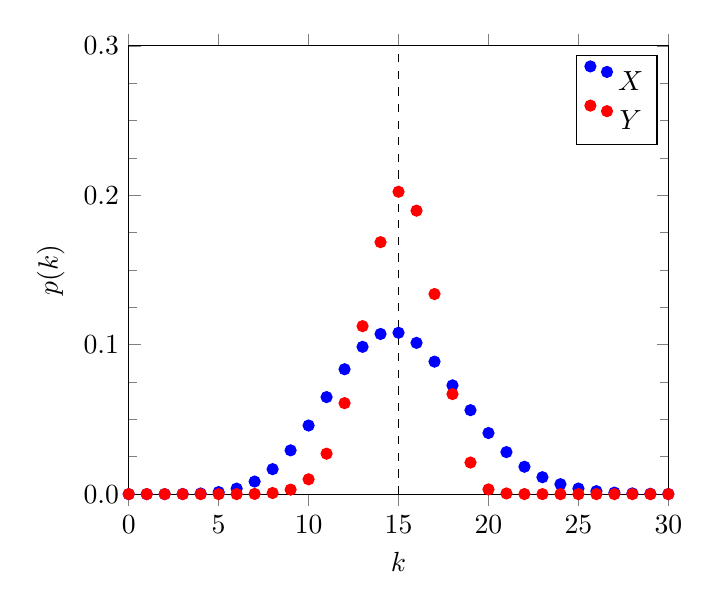
\begin{tikzpicture}[
                declare function={binom(\k,\n,\p)=\n!/(\k!*(\n-\k)!)*\p^\k*(1-\p)^(\n-\k);}
            ]
                \begin{axis}[
                    ybar,
                    xmin = 0, xmax = 30,
                    ymin = 0, ymax = 0.3,
                    minor y tick num = 3,
                    xlabel = {$k$},
                    ylabel = {$p(k)$},
                    samples at={0,...,50},
                    yticklabel style={
                        /pgf/number format/fixed,
                        /pgf/number format/fixed zerofill,
                        /pgf/number format/precision=1
                    }
                    ]

                    \addplot [only marks, blue] {binom(x,150,0.1)}; \addlegendentry{$X$}
                    \addplot [only marks, red] {binom(x,20,0.75)}; \addlegendentry{$Y$}
                    \draw[dashed] (axis cs:15,0) -- (axis cs:15,0.3);

                \end{axis}
            \end{tikzpicture}
        }

        \caption{Le due distribuzioni e la loro media comune.}
    \end{figure}

    Formalmente, diciamo che la \textbf{varianza} della variabile $X$ è maggiore da quella della variabile $Y$. La varianza è una misura di dispersione, ossia una misura di quanto un dato insieme di numeri si discosta (o \textit{varia}) dal suo valore medio. Se una v.a. assume valori lontani dalla sua media, la sua varianza sarà grande. Al contrario, se la variabile aleatoria rimane costante, la sua varianza sarà nulla. Nello specifico, la varianza è definita come il valore atteso del quadrato della variabile aleatoria centrata $X - \Exp[X]$.

    \begin{frameddefn}{Varianza}
        Data una v.a. $X$, definiamo la varianza di $X$, indicata con $\mathrm{Var}(X)$, come:
        \[\mathrm{Var}(X) = \Exp[(X-\Exp[X])^2]\]
    \end{frameddefn}

    Osserviamo facilmente che la varianza risulta essere una funzione non-negativa in quanto l'elevamento al quadrato ci assicura che tutti i valori siano positivi:
    \[\mathrm{Var}(X) = \Exp[(X-\Exp[X])^2] = \sum_{x \in X(\Omega)} (x-\Exp[X])^2 p_X(x) \geq 0\]

    Ma perchè proprio il valore atteso del quadrato del ricentramento della variabile con la sua media? Intuitivamente, i valori assunti dalla variabile aleatoria $Z = X - \Exp[X]$ corrispondono alle differenze tra i singoli valori di $X$ e la media. Elevando il tutto al quadrato, dunque la variabile $Z^2$, ognuna delle differenze assume valore non-negativo, permettendoci di considerarle come \curlyquotes{distanze}. Chiaramente, anche l'utilizzo del valore assoluto sarebbe sufficiente per raggiungere tale obiettivo, ma l'uso del quadrato ci permette di ottenere un'ulteriore proprietà: le differenze molto piccole -- ossia nell'intervallo aperto $(-1,1) \subset \R$ -- vengono \textit{sminuite} in quanto il loro quadrato sarà ancora più piccolo, mentre differenze molto grandi -- ossia al di fuori di tale intervallo -- vengono \textit{accentutate}.

    In molte occasioni, può tornare più utile la seguente riformulazione della varianza, equivalente alla definizione data.

    \begin{framedthm}{Varianza (2° def.)}
        Data una v.a. $X$ si ha che $\mathrm{Var}(X) = \Exp[X^2]-\Exp[X]^2$
    \end{framedthm}

    \begin{proof}
        Sia $\mu = \Exp[X]$. Tramite la linearità e l'idempotenza del valore atteso concludiamo facilmente che:
        \[\begin{split}
            \mathrm{Var}(X) &= \Exp[(X-\mu)^2] \\
            &= \Exp[X^2 - 2X\mu + \mu^2] \\
            &= \Exp[X^2]- 2\mu\Exp[X] + \Exp[\mu^2] \\
            &= \Exp[X^2]- 2\mu^2 + \mu^2 \\
            &= \Exp[X^2]- \Exp[X]^2 \\
        \end{split}\]
    \end{proof}

    Supponiamo ora di voler studiare quanto due variabili aleatorie $X$ ed $Y$ \textit{varino assieme}, cioè quanto i valori della prima vari in base ai valori della seconda. Questa misura viene detta \textbf{covarianza}.

    \begin{frameddefn}{Covarianza}
        Date due v.a. $X$ e $Y$, definiamo la covarianza tra $X$ e $Y$, indicata con $\mathrm{Cov}(X,Y)$, come:
        \[\mathrm{Cov}(X,Y) = \Exp[(X-\Exp[X])(Y-\Exp[Y])]\]
    \end{frameddefn}

    Dalla definizione di covarianza risulta immediato che $\mathrm{Cov}(X,X) = \mathrm{Var}(X)$, vale a dire che la varianza tra $X$ e se stessa corrisponda alla varianza stessa.

    Differentemente dalla varianza, la covarianza può anche assumere valori negativi. Difatti, è proprio il segno della covarianza tra due variabili aleatorie a descrivere la loro \textbf{correlazione}, ossia quanto ciascuna cambi in base al valore dell'altra.
    \begin{itemize}
        \item Se $\mathrm{Cov}(X,Y) > 0$ allora all'aumentare di $X$ aumenterà anche $Y$. Maggiore è il valore della covarianza, maggiore sarà l'aumento proporzionale.
        \item Se $\mathrm{Cov}(X,Y) = 0$ allora all'aumentare di $X$ non è detto che $Y$ aumenti. Quando la covarianza è 0, le due variabili vengono dette \textbf{incorrelate}.
        \item Se $\mathrm{Cov}(X,Y) < 0$ allora all'aumentare di $X$ diminuirà $Y$. Minore è il valore della covarianza, maggiore sarà l'aumento inversamente proporzionale.
    \end{itemize}

    Come per la varianza, anche la covarianza può essere espressa in forma alternativa.

    In molte occasioni, può tornare più utile la seguente riformulazione della varianza, equivalente alla definizione data.

    \begin{framedthm}{Covarianza (2° def.)}
        Date due v.a. $X$ e $Y$ si ha che $\mathrm{Cov}(X,Y) = \Exp[XY]-\Exp[X]\Exp[Y]$
    \end{framedthm}

    \begin{proof}
        Siano $\mu = \Exp[X]$ e $\eta = \Exp[Y]$. Tramite la linearità e l'idempotenza del valore atteso concludiamo facilmente che:
        \[\begin{split}
            \mathrm{Cov}(X,Y) &= \Exp[(X-\mu)(Y-\eta)] \\
            &= \Exp[XY - \eta X - \mu Y - \eta\mu] \\
            &= \Exp[XY] - \eta \mu- \mu \eta - \eta\mu \\
            &= \Exp[XY] - \Exp[X]\Exp[Y] \\
        \end{split}\]
    \end{proof}

    

    \subsection{Proprietà di varianza e covarianza}

    Poiché definita tramite il valore atteso, ci aspettiamo che anche la varianza goda di una proprietà di linearità. Tuttavia, la presenza dell'elevamento al quadrato non ci permette di ottenere una \curlyquotes{linearità pulita} come quella del valore atteso: la costante moltiplicativa viene elevata al quadrato mentre viene portata fuori dall'operatore e il termine costante viene eliminato. Questa proprietà viene detta \textbf{invarianza per traslazione}.

    \begin{framedthm}{Invarianza per traslazione della varianza}
        Data una v.a. $X$ e due valori $\alpha, \beta \in \R$ si ha che:
        \[\mathrm{Var}(\alpha X + \beta) = \alpha^2 \mathrm{Var}(X)\]
    \end{framedthm}

    \begin{proof}
        Applicando la seconda definizione di varianza abbiamo che:
        \[\begin{split}
            \mathrm{Var}(\alpha X+\beta) &= \Exp[(\alpha X + \beta)^2] - \Exp[\alpha X + \beta]^2 \\
            &= \Exp[\alpha^2 X^2 + 2 \alpha \beta X + \beta^2] - \Exp[\alpha X + \beta]^2 \\
        \end{split}\]

        Infine, per la linearità del valore atteso concludiamo che:
        \[\begin{split}
            \mathrm{Var}(\alpha X + \beta) &= \Exp[\alpha^2 X^2 + 2 \alpha \beta X + \beta^2] - \Exp[\alpha X + \beta]^2 \\
            &= \alpha^2 \Exp[X^2] + 2 \alpha \beta \Exp[X] + \beta^2 - (\alpha \Exp[X] + \beta)^2 \\
            &= \alpha^2 \Exp[X^2] + 2 \alpha \beta \Exp[X] + \beta^2 - \alpha^2 \Exp[X]^2 - 2\alpha \beta \Exp[X] - \beta^2 \\
            &= \alpha^2 (\Exp[X^2] - \Exp[X]^2) \\
            &= \alpha^2 \mathrm{Var}(X) \\
        \end{split}\]
    \end{proof}

    Similmente, anche per quanto riguarda la somma tra variabili aleatorie non possiamo stabilire una vera proprietà di linearità, ma solo una linearità parziale. In particolare, varianza della somma tra due v.a. è uguale alla somma delle varianze delle due v.a. e il doppio della loro covarianza.
    
    \begin{framedprop}{}
        Date due v.a. $X$ e $Y$, si ha che:
        \[\mathrm{Var}(X+Y) = \mathrm{Var}(X) + \mathrm{Var}(Y) + 2\mathrm{Cov}(X,Y)\]
    \end{framedprop}

    \begin{proof}
        Applicando la seconda definizione di varianza abbiamo che:
        \[\begin{split}
            \mathrm{Var}(X+Y) &= \Exp[(X+Y)^2] - \Exp[X+Y]^2 \\
            &= \Exp[X^2+2XY+Y^2] - (\Exp[X]+\Exp[Y])^2 \\
            &= \Exp[X^2]+2\Exp[XY]+\Exp[Y^2] - \Exp[X]^2 - 2\Exp[X]\Exp[Y] - \Exp[Y]^2 \\
            &= \mathrm{Var}(X) + \mathrm{Var}(Y) + 2\mathrm{Cov}(X,Y)
        \end{split}\]
    \end{proof}

    \begin{framedcor}{}
        Date due v.a. $X$ e $Y$ incorrelate, ossia con $\mathrm{Cov}(X,Y) = 0$, si ha che:
        \[\mathrm{Var}(X+Y) = \mathrm{Var}(X) + \mathrm{Var}(Y)\]
    \end{framedcor}

    Per quanto riguarda la covarianza, invece, possiamo stabilire una relazione ben più forte anche senza l'indipendenza o l'incorrelazione delle due variabili.

    \begin{framedthm}{}
        Date tre v.a. $X, Y, Z$ e due valori $\alpha,\beta \in \R$ si ha che:
        \[\mathrm{Cov}(\alpha X + \beta Y, Z) = \alpha \mathrm{Cov}(X,Z) + \beta \mathrm{Cov}(Y,Z)\] 
    \end{framedthm}

    \begin{proof}
        Applicando la seconda definizione di covarianza e le proprietà del valore atteso abbiamo che:
        \[\begin{split}
            \mathrm{Cov}(\alpha X + \beta Y, Z) &= \Exp[(\alpha X + \beta Y) Z] - \Exp[\alpha X + \beta Y]\Exp[Z] \\
            &= \Exp[\alpha XZ + \beta Y Z] - \Exp[\alpha X + \beta Y]\Exp[Z] \\
            &= \alpha \Exp[XZ] + \beta \Exp[YZ] - (\alpha \Exp[X] + \beta Y)\Exp[Z] \\
            &= \alpha \mathrm{Cov}(X,Z) + \beta \mathrm{Cov}(Y,Z) \\
        \end{split}\]
    \end{proof}

    Come visto nella \Cref{ind_exp_val}, quando due variabili aleatorie $X$ e $Y$ sono indipendenti tra loro si ha che $\Exp[XY] = \Exp[X]\Exp[Y]$. Questo ci permette di concludere immediatamente che, come da aspettarsi, due v.a. indipendenti sono anche incorrelate.

    \begin{framedthm}{}
        Date due v.a. $X$ ed $Y$, se le due variabili sono indipendenti tra loro allora sono anche incorrelate, ossia $\mathrm{Cov}(X,Y) = 0$.
    \end{framedthm}

    \begin{proof}
        Tramite la seconda definizione di covarianza concludiamo subito che:
        \[\mathrm{Cov}(X,Y) = \Exp[XY] - \Exp[X]\Exp[Y] = \Exp[X]\Exp[Y] - \Exp[X]\Exp[Y] = 0\]
    \end{proof}

    Similmente al caso del valore atteso, se le due variabili aleatorie sono dipendenti allora non è detto che esse siano correlate (positivamente o negativamente). Difatti, riprendendo lo stesso esempio con le v.a. $X, Y$ tali che $Y = X^2$, dove $X(\Omega) = \{-1,0,1\}$ e:
    \[\Pr[X = -1] = \frac{1}{5} \qquad \Pr[X = 0] = \frac{3}{5} \qquad \Pr[X = 1] = \frac{1}{5}\]

    Avevamo già concluso come $\Exp[X] = 0, \Exp[Y] = \frac{2}{5}$ e $\Exp[XY] = 0$, implicando che:
    \[\mathrm{Cov}(X,Y) = \Exp[XY] - \Exp[X]\Exp[Y] = 0 - 0 \cdot \frac{2}{5} = 0\]
    nonostante le due variabili siano dipendenti.
    
    \begin{framedobs}{}
        Date due v.a. $X$ e $Y$ dipendenti tra loro, non è detto che esse siano correlate, ossia che $\mathrm{Cov}(X,Y) \neq 0$
    \end{framedobs}

    \subsection{Varianze di distribuzioni note}

    Come nel per il valore atteso, è possibile trovare le varianze delle distribuzioni note in funzione dei loro parametri, permettendo un calcolo rapido. In particolare, rispetto al valore atteso, conoscere il valore finito delle varianze risulta di estrema comodità, poiché altrimenti sarebbe necessario calcolare ogni volta somme molto complesse.

    \begin{framedprop}{Varianza di una Bernoulliana}
        Data una v.a. $X$ tale che $X \sim \mathcal{B}(p)$, si ha che:
        \[\mathrm{Var}(X) = p(1-p)\]
    \end{framedprop}

    \begin{proof}
        Trattandosi di una Bernoulliana, sappiamo che $\Exp[X] = p$. Per tanto, abbiamo che:
        \[\begin{split}
            \mathrm{Var}(X) &= \Exp[X^2] - \Exp[X]^2 \\
            &= 0^2 \cdot \Pr[X = x] + 1^2 \Pr[X=x] - p^2 \\
            &= p-p^2 \\
            &= p(1-p) \\
        \end{split}\]
    \end{proof}

    \begin{framedprop}{Varianza di una uniforme discreta}
        Data una v.a. $X$ tale che $X \sim \mathcal{U}\{a,b\}$, si ha che:
        \[\mathrm{Var}(X) = \frac{(b-a)(b-a+2)}{12}\]
    \end{framedprop}

    \begin{proof}
        Trattandosi di un'uniforme discreta abbiamo che:
        \[\begin{split}
            \Exp[X^2] &= \sum_{k =a}^b k^2 \Pr[X = k]\sum_{k = a}^b k^2 \frac{1}{b-(a-1)} \\
            &= \frac{1}{b-(a-1)} \rbk{\sum_{k = 1}^{b} k^2 - \sum_{k}^{a-1} k^2} \\
            &= \frac{1}{b-a+1} \rbk{\frac{b(b+1)(2b+1)}{6}- \frac{(a-1)a(2(a-1)+1)}{6}}\\
            &= \frac{2b^3+3b^2+b - 2a^3+3a^2-a}{6(b-a+1)} \\
        \end{split}\]

        Dunque, concludiamo che:
        \[\begin{split}
            \mathrm{Var}(X) &= \Exp[X^2] - \Exp[X]^2 \\
            &= \frac{2b^3+3b^2+b - 2a^3+3a^2-a}{6(b-a+1)} - \frac{a^2+2ab+b^2}{4} \\
            &= \frac{(b-a)(b-a+2)}{12}
        \end{split}\]
    \end{proof}
    
    \begin{framedprop}{Varianza di una binomiale}
        Data una v.a. $X$ tale che $X \sim \mathrm{Bin}(n,p)$, si ha che:
        \[\mathrm{Var}(X) = np\]
    \end{framedprop}

    \begin{proof}
        Siano $X_1, \ldots, X_n \sim \mathcal{B}(p)$ le v.a. che definiscono il processo di Bernoulli descritto da $X$, dunque $X = X_1 + \ldots + X_n$. Poiché $X_1, \ldots, X_n$ sono indipendenti tra loro, sappiamo che:
        \[\mathrm{Var}(X) = \mathrm{Var}(X_1 + \ldots + X_n) = \mathrm{Var}(X_1) + \ldots + \mathrm{Var}(X_n) = n \mathrm{Var}(X_1)\]

        Infine, poiché $X_1$ è una Bernoulliana concludiamo immediatamente che $\mathrm{Var}(X_1) = p(1-p)$ e dunque che $\mathrm{Var}(X) = np(1-p)$
    \end{proof}

    \begin{framedprop}{Varianza di una geometrica}
        Data una v.a. $X$ tale che $X \sim \mathrm{Geom}(p)$, si ha che:
        \[\mathrm{Var}(X) = \frac{1-p}{p^2}\]
    \end{framedprop}

    \begin{proof}
        Trattandosi di una geometrica abbiamo che:
        \[\begin{split}
            \Exp[X^2] &= \sum_{k = 1}^{+\infty} k^2 \Pr[X = k] = \sum_{k = 1}^{+\infty} k^2 (1-p)^{k-1} p = p \sum_{k = 1}^{+\infty} k^2 (1-p)^{k-1}\\
        \end{split}\]

        Procedendo in modo del analogo al calcolo di $\Exp[X]$ già svolto in precedenza, osserviamo come ogni termine $k$-esimo della somma infinita corrisponda alla derivata in $p$ di $-k(1-p)^k$. Per tanto, abbiamo che:
        \[\begin{split}
            \Exp[X^2] &= p\sum_{k = 1}^{+\infty} k^2 (1-p)^{k-1} \\
            &= p \sum_{k = 1}^{+\infty} \frac{\diff}{\diff p} \rbk{-k (1-p)^{k}} \\
            &= p \, \frac{\diff}{\diff p} \rbk{- \sum_{k = 1}^{+\infty} k (1-p)^{k}}  \\
            &= p \, \frac{\diff}{\diff p} \rbk{- \frac{1-p}{p} \sum_{k = 1}^{+\infty} k (1-p)^{k-1}p}  \\
        \end{split}\]

        Notiamo quindi che la somma ottenuta corrisponda al valore atteso $\Exp[X]$, implicando che:
        \[\begin{split}
        \Exp[X^2] &= p \, \frac{\diff}{\diff p} \rbk{- \frac{1-p}{p} \Exp[X]} \\
        &= p \, \frac{\diff}{\diff p} \rbk{ \frac{p-1}{p^2}} \\
        &= p \, \frac{2-p}{p^3} \\
        &= \frac{2-p}{p^2} \\
        \end{split}\]

        Concludiamo quindi che:
        \[\begin{split}
            \mathrm{Var}(X) &= \Exp[X^2] - \Exp[X]^2 = \frac{2-p}{p^2} - \frac{1}{p^2} = \frac{1-p}{p^2}
        \end{split}\]
    \end{proof}

    \begin{framedprop}{Varianza di una ipergeometrica}
        Data una v.a. $X$ tale che $X \sim \mathrm{Hyp}(N,K,n)$, si ha che:
        \[\mathrm{Var}(X) = \frac{nK(N-n)(N-K)}{N^2(N-1)}\]
    \end{framedprop}

    \begin{proof}
        Trattandosi di una ipergeometrica abbiamo che:
        \[\begin{split}
            \Exp[X^2] &= \sum_{k = 0}^n k^2 \Pr[X = k] = \sum_{k = 0}^n k^2 \, \frac{\binom{K}{k} \binom{N-K}{n-k}}{\binom{N}{n}} \\
        \end{split}\]

        Osserviamo che il primo termine della sommatoria può essere rimosso in quanto contiene un prodotto con $k^2 = 0$, ottenendo:
        \[\Exp[X] = \sum_{k = 1}^n k^2 \, \frac{\binom{K}{k} \binom{N-K}{n-k}}{\binom{N}{n}}\]

        A questo punto, procedendo in modo del analogo al calcolo di $\Exp[X]$ già svolto in precedenza, osserviamo come:
        \[\begin{split}
            \Exp[X^2] &= \sum_{k = 1}^n k^2 \, \frac{\binom{K}{k} \binom{N-K}{n-k}}{\binom{N}{n}} = \frac{nK}{N} \sum_{k = 1}^n k \frac{\binom{K-1}{k-1} \binom{N-1-(K-1)}{n-1-(k-1)}}{\binom{N-1}{n-1}}\\
        \end{split}\]

        Poniamo quindi $j = k-1$ per riaggiustare gli indici della sommatoria:
        \[\begin{split}
            \Exp[X^2] &= \frac{nK}{N} \sum_{j = 0}^n (j+1) \frac{\binom{K-1}{j} \binom{N-1-(K-1)}{n-1-j}}{\binom{N-1}{n-1}}\\
        \end{split}\]

        Notiamo quindi che la somma ottenuta corrisponde al valore atteso $\Exp[Y+1]$ con $Y \sim \mathrm{Hyp}(N-1, K-1, n-1)$, implicando che:
        \[\begin{split}
            \Exp[X^2] &= \frac{nK}{N} \Exp[Y+1] = \frac{nK}{N}\rbk{\frac{(n-1)(K-1)}{N-1} + 1}
        \end{split}\]

        Concludiamo quindi che:
        \[\begin{split}
            \mathrm{Var}(X) &= \Exp[X^2] - \Exp[X]^2 \\
            &= \frac{nK}{N}\rbk{\frac{(n-1)(K-1)}{N-1} + 1} - \rbk{\frac{nK}{N}}^2 \\
            &= \frac{nK(N-n)(N-K)}{N^2(N-1)}
        \end{split}\]
    \end{proof}

    \begin{framedprop}{Varianza di una Poissoniana}
        Data una v.a. $X$ tale che $X \sim \mathrm{Poiss}(\lambda)$, si ha che:
        \[\mathrm{Var}(X) = \lambda\]
    \end{framedprop}

    \begin{proof}
        Trattandosi di una Poissoniana abbiamo che:
        \[\begin{split}
            \Exp[X^2] &= \sum_{k=0}^{\infty} k^2 \Pr[X = k] = \sum_{k=0}^{\infty} k^2 e^{-\lambda} \frac{\lambda^k}{k!}
        \end{split}\]

        Osserviamo che il primo termine della sommatoria può essere rimosso in quanto contiene un prodotto con $k^2 = 0$: 
        \[\begin{split}
            \Exp[X^2] &= e^{-\lambda} \lambda \sum_{k=1}^{\infty} k^2 e^{-\lambda} \frac{\lambda^{k-1}}{k!} = \lambda \sum_{k=1}^{\infty} k e^{-\lambda} \frac{\lambda^{k-1}}{(k-1)!} \\
        \end{split}\]

        Poniamo quindi $j = k-1$ per riaggiustare gli indici della sommatoria:
        \[\Exp[X^2] = \lambda \sum_{j=0}^{\infty} (j+1) e^{-\lambda} \frac{\lambda^{j}}{j!}\]
        
        Notiamo quindi che la somma ottenuta corrisponda al valore atteso $\Exp[X+1]$, concludendo immediatamente che:
        \[ \Exp[X^2] = \lambda \Exp[X+1] = \lambda^2 + \lambda\]

        Concludiamo quindi che:
        \[\mathrm{Var}(X) = \mathrm{Exp}[X^2] - \Exp[X]^2 = \lambda^2 + \lambda - \lambda^2 = \lambda\]
    \end{proof}

    \begin{framedprop}{Varianza di una Pascaliana}
        Data una v.a. $X$ tale che $X \sim \mathrm{Pasc}(n,p)$, si ha che:
        \[\mathrm{Var}(X) = \frac{n(1-p)}{p^2}\]
    \end{framedprop}

    \begin{proof}
        Siano $\Delta_1, \ldots, \Delta_n \sim \mathrm{Geom}(p)$ le v.a. che definiscono il tempo di $n$-esimo successo $T_n = X$. Tramite la linearità del valore atteso e il valore atteso noto di una geometrica, concludiamo immediatamente che:
        \[\mathrm{Var}(X) = \mathrm{Var}[\Delta_1 + \ldots + \Delta_n] = \mathrm{Var}[\Delta_1] + \ldots + \mathrm{Var}[\Delta_n] = \frac{n(1-p)}{p^2}\]
    \end{proof}

    \section{Standardizzazione di variabili aleatorie}
    \label{standard}

    In alcuni casi, potremmo non essere interessati allo sminuimento e all'accentuamento delle differenze ottenuto tramite l'elevamento a potenza. Per \textit{attenuare} tale processo -- ma non invertire -- preservando il segno positivo viene considerata la radice quadrata della varianza, anche detta \textbf{deviazione standard} (o \textit{scarto quadratico medio}, o \textit{scarto tipo}). In questo modo, la deviazione standard risulta essere una misura \textit{più grezza} per il discostamento dalla media.

    \begin{frameddefn}{Deviazione standard}
        Data una v.a. $X$, definiamo la deviazione standard di $X$, indicata con $\sigma_X$ (o direttamente $\sigma$ se il contesto non è ambiguo), come:
        \[\sigma_X = \sqrt{\mathrm{Var}(X)}\]
    \end{frameddefn}
    
    Per dare un'intuizione dietro l'uso della deviazione standard, consideriamo la variabile $X \sim \mathrm{Bin}(36, 0.5)$. Essendo una distribuzione nota, sappiamo che:
    \[\Exp[X] = 36 \cdot 0.5 = 18 \qquad\quad \sigma = \sqrt{\mathrm{Var}} = \sqrt{36 \cdot 0.5 \cdot 0.5} = 3\]

    Una volta calcolata la deviazione standard, essa può essere utilizzata per sapere il \textit{discostamento dalla media}. Comunemente, è di interesse sapere la probabilità che la variabile $X$ di discosti entro $m$ deviazioni dalla media, vale a dire la probabilità $\Pr[\mu - m\sigma \leq X \leq \mu + m\sigma]$, dove $\mu = \Exp[X]$.

    \begin{figure}[H]
        \centering
        \resizebox{0.6\textwidth}{!}{
            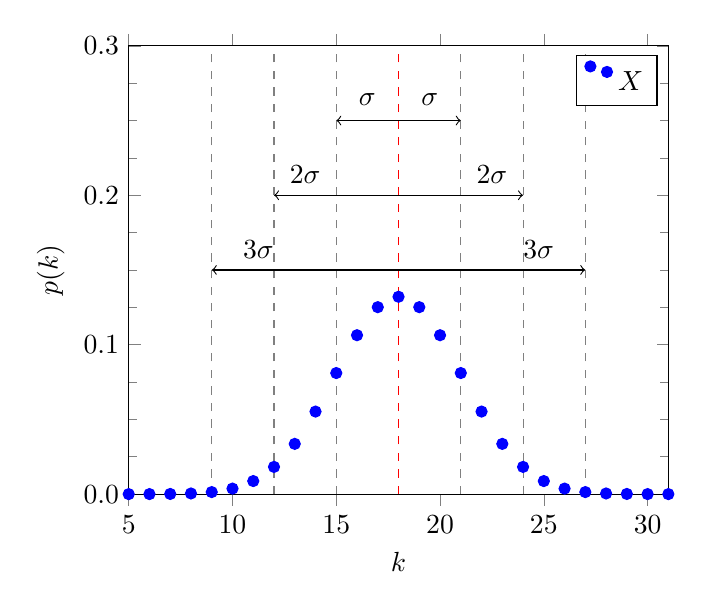
\begin{tikzpicture}[
                declare function={binom(\k,\n,\p)=\n!/(\k!*(\n-\k)!)*\p^\k*(1-\p)^(\n-\k);}
            ]
                \begin{axis}[
                    ybar,
                    xmin = 5, xmax = 31,
                    ymin = 0, ymax = 0.3,
                    minor y tick num = 3,
                    xlabel = {$k$},
                    ylabel = {$p(k)$},
                    samples at={0,...,50},
                    yticklabel style={
                        /pgf/number format/fixed,
                        /pgf/number format/fixed zerofill,
                        /pgf/number format/precision=1
                    }
                    ]

                    \addplot [only marks, blue] {binom(x,36,0.5)}; \addlegendentry{$X$}
                    \draw[dashed, red] (axis cs:18,0) -- (axis cs:18,0.3); \addlegendentry{$\Exp[X]$}

                    \draw[->] (axis cs:18,0.25) -- node[yshift = 7.5]{$\sigma$}(axis cs:15,0.25);
                    \draw[->] (axis cs:18,0.25) -- node[yshift = 7.5]{$\sigma$} (axis cs:21,0.25);
                    \draw[dashed, gray] (axis cs:15,0) -- (axis cs:15,0.3);
                    \draw[dashed, gray] (axis cs:21,0) -- (axis cs:21,0.3);

                    \draw[->] (axis cs:18,0.2) -- node[yshift = 7.5, near end]{$2\sigma$}(axis cs:12,0.2);
                    \draw[->] (axis cs:18,0.2) -- node[yshift = 7.5, near end]{$2\sigma$} (axis cs:24,0.2);
                    \draw[dashed, gray] (axis cs:12,0) -- (axis cs:12,0.3);
                    \draw[dashed, gray] (axis cs:24,0) -- (axis cs:24,0.3);

                    \draw[->] (axis cs:18,0.15) -- node[yshift = 7.5, near end]{$3\sigma$}(axis cs:9,0.15);
                    \draw[->] (axis cs:18,0.15) -- node[yshift = 7.5, near end]{$3\sigma$} (axis cs:27,0.15);
                    \draw[dashed, gray] (axis cs:9,0) -- (axis cs:9,0.3);
                    \draw[dashed, gray] (axis cs:27,0) -- (axis cs:27,0.3);
                \end{axis}
            \end{tikzpicture}
        }

        \caption{La distribuzione della variabile $X$ in esempio e i suoi intervalli di deviazione.}
    \end{figure}

    Il \textbf{punteggio standard} (o \textit{z-score}) di ogni valore $x$ assumibile da una variabile aleatoria $X$ corrisponde al numero di deviazioni standard per cui $x$ si discosta dal valore atteso $\Exp[X] = \mu$. L'insieme di tutti i punteggi standard da vita ad una variabile aleatoria $Z$ detta \textbf{standardizzata} di $X$.

    \begin{frameddefn}{Standardizzata di una variabile aleatoria}
        Data una v.a. $X$ con $\mathrm{Var}(X) > 0$, la standardardizzata di $X$ è la v.a. $Z$ definita da $X = \sigma_X Z + \mu$, dove $\Exp[X] = \mu$.
    \end{frameddefn}

    \begin{figure}[H]
        \centering
        \resizebox{0.6\textwidth}{!}{
            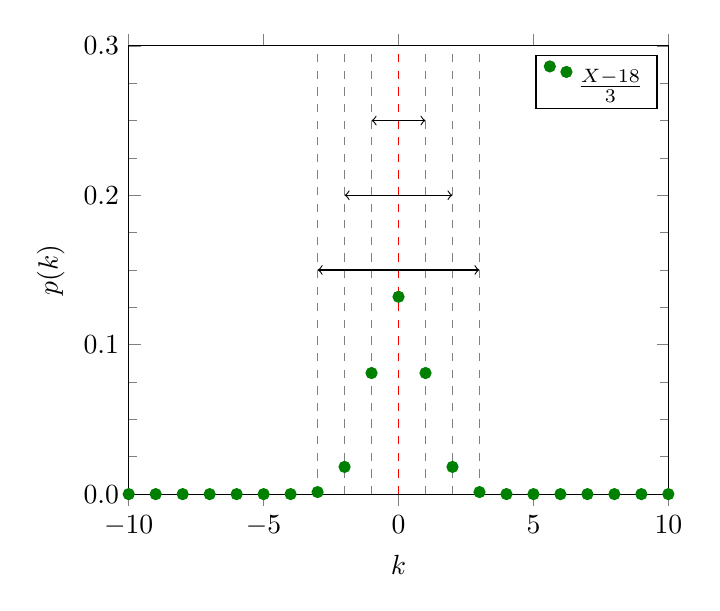
\begin{tikzpicture}[
                declare function={binom(\k,\n,\p)=\n!/(\k!*(\n-\k)!)*\p^\k*(1-\p)^(\n-\k);}
            ]
                \begin{axis}[
                    ybar,
                    xmin = -10, xmax = 10,
                    ymin = 0, ymax = 0.3,
                    minor y tick num = 3,
                    xlabel = {$k$},
                    ylabel = {$p(k)$},
                    samples at={-10,...,10},
                    yticklabel style={
                        /pgf/number format/fixed,
                        /pgf/number format/fixed zerofill,
                        /pgf/number format/precision=1
                    }
                    ]

                    \addplot [only marks, Green] {binom(3*x+18, 36,0.5)}; \addlegendentry{$\frac{X-18}{3}$}
                    \draw[dashed, red] (axis cs:0,0) -- (axis cs:0,0.3); \addlegendentry{$Z$}

                    \draw[->] (axis cs:0,0.25) -- (axis cs:-1,0.25);
                    \draw[->] (axis cs:0,0.25) -- (axis cs:1,0.25);
                    \draw[dashed, gray] (axis cs:-1,0) -- (axis cs:-1,0.3);
                    \draw[dashed, gray] (axis cs:1,0) -- (axis cs:1,0.3);

                    \draw[->] (axis cs:0,0.2) -- (axis cs:-2,0.2);
                    \draw[->] (axis cs:0,0.2) --  (axis cs:2,0.2);
                    \draw[dashed, gray] (axis cs:-2,0) -- (axis cs:-2,0.3);
                    \draw[dashed, gray] (axis cs:2,0) -- (axis cs:2,0.3);

                    \draw[->] (axis cs:0,0.15) -- (axis cs:-3,0.15);
                    \draw[->] (axis cs:0,0.15) -- (axis cs:3,0.15);
                    \draw[dashed, gray] (axis cs:-3,0) -- (axis cs:-3,0.3);
                    \draw[dashed, gray] (axis cs:3,0) -- (axis cs:3,0.3);
                \end{axis}
            \end{tikzpicture}
        }

        \caption{La standardizzata della variabile $X$ in esempio.}
    \end{figure}


    Il nome deviazione standard deriva quindi dall'uso di tale misura per descrivere quanto una variabile aleatoria $X$ si discosti dalla sua versione standardizzata, ossia la variabile aleatoria $Z$. In particolare, osserviamo che ogni standardizzata ha per definizione valore atteso ma con $\Exp[Z] = 0$ e varianza $\mathrm{Var}(Z) = 1$.

    \begin{framedthm}{}
        Data una v.a $X$ e la sua standardizzata $Z$, vale che $\Exp[Z] = 0$ e $\mathrm{Var}(Z) = 1$
    \end{framedthm}

    \begin{proof}
        Sia $\mu = \Exp[X]$. Per linearità del valore atteso si ha che:
        \[\Exp[Z] = \Exp\sbk{\frac{X - \mu}{\sigma_X}} = \frac{\Exp[X]-\mu}{\sigma_X} = \frac{0}{\sigma_X} = 0 \]

        Similmente, per invarianza per traslazione della varianza abbiamo che:
        \[\mathrm{Var}(Z) = \mathrm{Var}\rbk{\frac{X - \mu}{\sigma_X}} = \frac{\mathrm{Var}(X)}{\sigma_X^2} =  1\]
    \end{proof}
    

    \addtocontents{toc}{\protect\newpage}

    \chapter{Variabili aleatorie continue}

    \section{Dal discreto al continuo}

    Dopo aver discusso a pieno le v.a. discrete, siamo ora pronti a spostare la nostra al caso delle \textbf{variabili aleatorie continue}. A differenza delle variabili aleatorie discrete, che possono prendere soltanto un insieme finito o numerabile di valori, nel caso continuo \underline{non è possibile} attribuire probabilità ai singoli punti. Infatti, in un insieme continuo di valori, esistono infiniti possibili risultati: la probabilità che la variabile assuma \textbf{esattamente} un certo valore è quindi nulla. In altre parole, per una variabile aleatoria continua $X$ si ha \underline{sempre} che $\Pr[X = x] = 0$ per ogni $x \in \R$. 

    Per questo motivo, la probabilità non si definisce sui singoli valori, ma su \textbf{intervalli} di valori. Ciò significa che ha senso parlare, ad esempio, solo ed esclusivamente della probabilità che una variabile sia compresa tra 1 e 2, e non della probabilità che valga precisamente 1,5. Per esprimere queste probabilità si introduce la \textbf{funzione di densità di probabilità} $\rho_X : \R \to [0,1] \subset \R$. Essa è una funzione non negativa tale che la probabilità che la variabile assuma un valore     nell'intervallo $I \subset \R$ è data dall'integrale dell'area sottesa alla curva di $\rho_X(x)$ su quell'intervallo.

    \begin{frameddefn}{Variabile aleatoria continua}
        Una v.a. $X$ è detta continua se esiste una funzione di densità di probabilità $\rho_X : \R \to [0, 1]$ tale che per ogni intervallo $I \subseteq \R$ si abbia che:
        \[\Pr[X \in I] = \int_I \rho_X(t) \, \diff t\]

        \textit{Nota}: il simbolo $\rho$ corrisponde al Rho greco minuscolo, non alla lettera $p$
    \end{frameddefn}

    Chiaramente, $\rho_X(x)$ deve anche soddisfare la \textit{condizione di normalizzazione} affinché $X$ sia una variabile aleatoria valida, ossia:
    \[\int_{-\infty}^{+\infty} \rho_X(t) \, \diff t = 1\]

    Supponiamo che una lampadina venga accesa e si voglia modellare il tempo $X$ (misurato in ore) fino al suo guasto. È evidente che $X$ può assumere qualsiasi valore reale positivo, vale a dire non ci sono \curlyquotes{buchi} tra i valori possibili. Ci viene detto che $X$ è descritto dalla seguente funzione di densità di probabilità:
    \[\rho_X(x) = \soe{ll}{
        e^{-x} & \text{se } x \geq 0 \\
        0 & \text{altrimenti} \\
    }\]

    La probabilità che la lampadina duri tra le 1 e le 2 ore è quindi data da:
    \[\Pr[X \in [1,2]] = \int_{1}^{2} e^{-t} \, \diff t = \frac{e-1}{e^2} \approx 0.23\]

    \begin{figure}[H]
        \centering
        \resizebox{0.6\textwidth}{!}{
            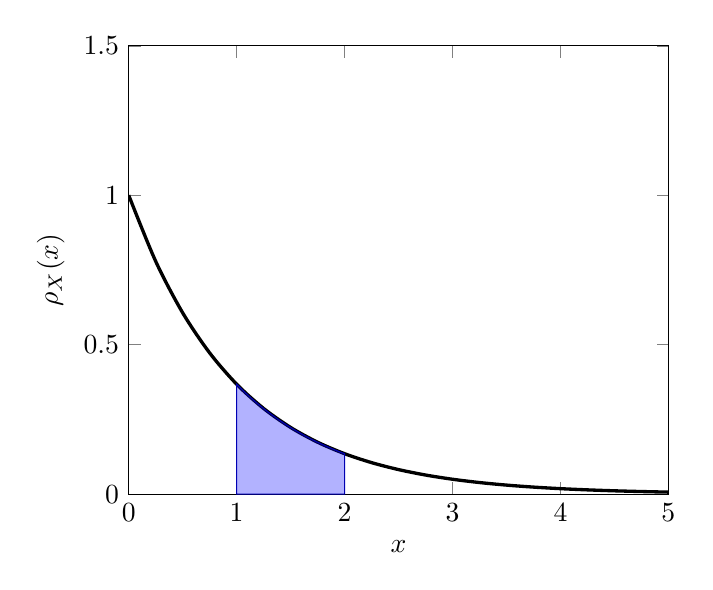
\begin{tikzpicture}[
                declare function={expdist(\x,\lambda)=\lambda*e^(-\lambda*\x);}
            ]
                \begin{axis}[
                    xlabel={$x$},
                    ylabel={$\rho_X(x)$},
                    domain=0:6,
                    ymin=0, ymax=1.5,
                    xmin=0, xmax=5
                ]

                    \addplot [very thick, smooth, black] {expdist(x,1)};
                    \addplot [
                        fill=blue,
                        fill opacity=0.3,
                        draw=blue!70!black,
                        domain=1:2
                    ] {expdist(x,1)} \closedcycle;
                \end{axis}
            \end{tikzpicture}
        }

        \caption{La funzione di densità discreta $\rho_X(x) = e^{-x}$. L'area evidenziata corrisponde alla probabilità $\Pr[X \in [1,2]$].}
    \end{figure}

    Nel caso di intervalli aperti, quindi, è necessario tratta l'integrale come un limite in cui ci si avvicina all'estremo aperto, come ad esempio:
    \[\Pr[X \in (1,2]] = \lim_{a \to 1^+} \int_{a}^2 e^{-t} \diff t\]
    \[\Pr[X \in [1, +\infty)] = \lim_{b \to +\infty} \int_1^{b} e^{-t} \diff t\] 

    Come nel caso discreto, per le variabili aleatorie continue è possibile individuare un analogo della \textbf{funzione di ripartizione}. In questo caso, è facile vedere che $F_X(x) = \Pr[X \leq x]$ corrisponda alla probabilità che la variabile assuma un valore nell'intervallo $(-\infty, x]$.
    \[F_X(x) = \Pr[X \leq x] = \Pr[X \in (-\infty, x]] = \int_{-\infty}^x \rho_X(t) \, \diff t\]

    Infine, diamo anche la definizione analoga di v.a. continue indipendenti.

    \begin{frameddefn}{Indipendenza tra v.a. continue}
        Diciamo che $n$ v.a. continue $X_1, \ldots, X_n$ sono indipendenti quando per ogni sottoinsieme $I \subseteq \{1,\ldots, n\}$, per ogni $a_1, \ldots, a_n \in \R$ ed ogni $b_1, \ldots, b_n \in \R$ si ha che:

        \[\Pr\sbk{\bigcap_{i \in I} a_i \leq X_i \leq b_i} = \prod_{i \in I} \Pr[a_i \leq X_i \leq b_i]\]

    \end{frameddefn}

    Anche nel caso continuo, quando due v.a. $X$ e $Y$ sono indipendenti si ha che $F_{X,Y}(x) = F_X(x)F_Y(x)$. Infine, introduciamo l'analogo continuo del \textbf{valore atteso}.

    \begin{frameddefn}{Valore atteso (v.a. continue)}
        Data una v.a. continua $X$, definiamo il valore atteso di $X$, indicato con $\Exp[X]$, come:
        \[\Exp[X] = \int\limits_{-\infty}^{+\infty} t \rho_X(t) \, \diff t\]
    \end{frameddefn}

    Ovviamente, il valore atteso delle variabili aleatorie continue preserva tutte le proprietà del normale valore atteso, ossia:
    \begin{itemize}
        \item \textit{Linearità}: $\Exp[\alpha X+\beta Y] = \alpha\Exp[X]+\beta \Exp[Y]$
        \item \textit{Monotonia}: $\Exp[X] \geq \Exp[Y]$ se $X \geq Y$
        \item \textit{Idempotenza}: $\Exp[\Exp[X]] = \Exp[X]$
        \item \textit{Legge dello statistico inconsapevole}: \[\Exp[f(X)] = \int_{-\infty}^{+\infty} f(x) \rho_X(x) \, dx\]
    \end{itemize}
    
    Omettiamo le loro dimostrazioni in quanto simili al caso discreto. Per quanto riguarda la \textbf{varianza} e la \textbf{covarianza}, invece, le definizioni restano analoghe, dunque anche le loro proprietà.
    
    \section{Distribuzioni continue come limite di discrete}

    \subsection{Distribuzione uniforme continua}

    Come per le v.a. discrete, il primo tipo di v.a. continua che introducialo è la \textbf{distribuzione uniforme continua}. Questo tipo di variabile non è altro che l'analogo continuo della distribuzione uniforme discreta: la probabilità è \textit{uniforme} su un intervallo $[a,b] \subset \R$, invece che su un intervallo $\{a, \ldots, b\} \subset \Z$.
    
    \begin{frameddefn}{Distribuzione uniforme continua}
        Una v.a. $X$ è detta a distribuzione uniforme continua di parametri $a$ e $b$, indicato con $X \sim \mathcal{U}[a,b]$, quando tutti i valori dell'intervallo $[a,b] \subset \R$ sono equiprobabilmente assumibili da $X$.

        Per ogni v.a $X \sim \mathcal{U}[a,b]$ vale che:
        \begin{itemize}
            \item $X(\Omega) = [a,b]$
            \item La funzione di densità di probabilità è dettata da:
            \[\rho_X(x) = \soe{ll}{
                \frac{1}{b-a} & \text{se } a \leq x \leq b \\
                0 & \text{altrimenti}
            }\]
        \end{itemize}
    \end{frameddefn}

    \begin{figure}[H]
        \centering
        \resizebox{0.6\textwidth}{!}{
            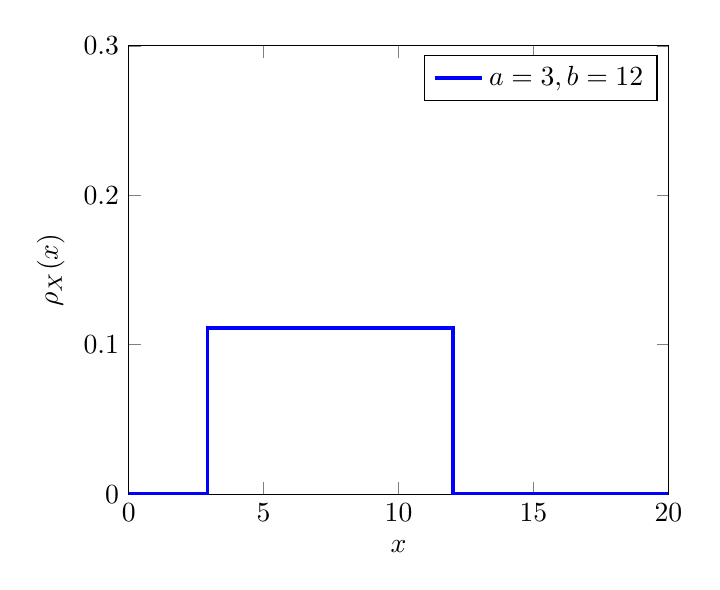
\begin{tikzpicture}[
                declare function={uniform(\x,\xl,\xu)= (\x>\xl)*(\x<\xu)*1/(\xu-\xl);}
            ]
            \begin{axis}[
                xlabel={$x$},
                ylabel={$\rho_X(x)$},
                domain=0:20,
                ymin=0, ymax=0.3,
                xmin=0, xmax=20,
                samples=100,
                const plot mark mid,
            ]

                \addplot [very thick, blue] {uniform(x,3,12)}; \addlegendentry{$a = 3, b = 12$}
            \end{axis}
            \end{tikzpicture}
        }

        \caption{Funzioni di densità di probabilità di una distribuzioni uniforme continua.}
    \end{figure}

    \begin{framedprop}{}
        Data una v.a. $X \sim \mathcal{U}[a,b]$ si ha che:
        \begin{itemize}
            \item $\displaystyle F_X(x) = \soe{ll}{
                0 & \text{se } x < a \\
                \dfrac{x-a}{b-a} & \text{se } a \leq x \leq b \\
                1 & \text{se } x > b \\
            }$
            \item $\Exp[X] = \dfrac{a+b}{2}$
            \item $\mathrm{Var}(X) = \dfrac{(b-a)^2}{12}$
        \end{itemize}
    \end{framedprop}

    \begin{proof} \,
        
        \begin{itemize}
            \item Per definzione abbiamo che:
            \[F_X(x) = \int_{-\infty}^x \frac{1}{b-a} \, \diff t = \soe{ll}{
                0 & \text{se } x < a \\
                \dfrac{x-a}{b-a} & \text{se } a \leq x \leq b \\
                1 & \text{se } x > b \\
            }\]

            \item Trattandosi di una uniforme continua abbiamo che:
            \[\Exp[X] = \int_{-\infty}^{+\infty} t \frac{1}{b-a} \, \diff t = \frac{1}{b-a} \int_a^b t \, \diff t = \frac{b^2-a^2}{2(b-a)} = \frac{a+b}{2}\]

            \item Trattandosi di una uniforme continua abbiamo che:
            \[\Exp[X^2] = \int_{-\infty}^{+\infty} t^2 \frac{1}{b-a} \, \diff t = \frac{1}{b-a} \int_a^b t^2 \, \diff t = \frac{b^3-a^3}{3(b-a)} = \frac{b^2+ab+a^2}{3}\]

            Concludendo quindi che:
            \[\mathrm{Var}(X) = \Exp[X^2] - \Exp[X]^2 = \frac{b^2+ab+a^2}{3} - \frac{b^2+2ab+a^2}{4} = \frac{(b-a)^2}{12}\]
        \end{itemize}
    \end{proof}

    \newpage

    \subsection{Distribuzione esponenziale}

    La \textbf{distribuzione esponenziale} è una distribuzione continua che descrive il tempo che intercorre tra due eventi consecutivi in un processo che avviene in modo casuale e continuo nel tempo, con una frequenza media costante e indipendente dal passato. È ampiamente utilizzata in contesti come l'affidabilità dei sistemi, la teoria delle code e i modelli di decadimento fisico. Dalla descrizione, risulta intuitivo considerare la distribuzione esponenziale come l'analogo continuo della \textit{distribuzione geometrica}, dove il tempo intercorso tra due eventi consecutivi corrisponde al numero di tentativi prima di un secondo successo.

    \begin{frameddefn}{Distribuzione esponenziale}
        Una v.a. $X$ è detta a distribuzione esponenziale di parametro $\lambda$, indicato con $X \sim \mathrm{Exp}(\lambda)$, quando descrive il tempo che intercorre tra due eventi consecutivi in un processo che avviene in modo casuale e continuo nel tempo, con una frequenza media costante e indipendente dal passato.

        Per ogni v.a $X \sim \mathrm{Exp}(\lambda)$ vale che:
        \begin{itemize}
            \item $X(\Omega) = [0,+\infty)$ e $\lambda > 0$
            \item La funzione di densità di probabilità è dettata da:
            \[\rho_X(x) = \lambda e^{-\lambda x}\]
        \end{itemize}
    \end{frameddefn}

    \begin{figure}[H]
        \centering
        \resizebox{0.6\textwidth}{!}{
            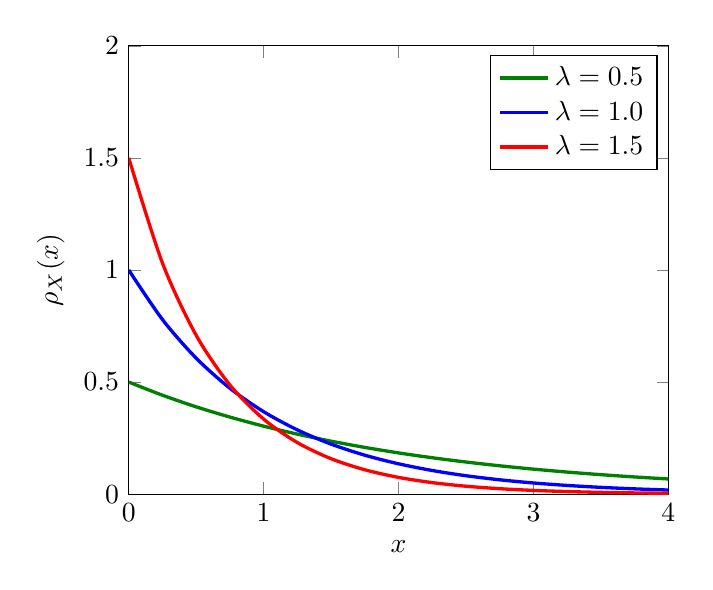
\begin{tikzpicture}[
                declare function={expdist(\x,\lambda)=\lambda*e^(-\lambda*\x);}
            ]
            \begin{axis}[
                xlabel={$x$},
                ylabel={$\rho_X(x)$},
                domain=0:6,
                ymin=0, ymax=2,
                xmin=0, xmax=4
            ]

                \addplot [very thick, smooth, Green] {expdist(x,0.5)}; \addlegendentry{$\lambda = 0.5$}
                \addplot [very thick, smooth, blue] {expdist(x,1.0)}; \addlegendentry{$\lambda = 1.0$}
                \addplot [very thick, smooth, red] {expdist(x,1.5)}; \addlegendentry{$\lambda = 1.5$}
            \end{axis}
            \end{tikzpicture}
        }

        \caption{Funzioni di densità di probabilità di tre distribuzioni esponenziali.}
    \end{figure}

    \begin{framedprop}{}
        Data una v.a. $X \sim \mathrm{Exp}(\lambda)$ si ha che:
        \begin{itemize}
            \item $\displaystyle F_X(x) = \soe{ll}{
                0 & \text{se } x < 0 \\
                1-e^{-\lambda x} & \text{se } x \geq 0 \\
            }$
            \item $\Exp[X] = \dfrac{1}{\lambda}$
            \item $\mathrm{Var}(X) = \dfrac{1}{\lambda^2}$
        \end{itemize}
    \end{framedprop}

    \begin{proof} \,
        
        \begin{itemize}
            \item Per $x < 0$ il risultato è banale. Per $x \geq 0$ invece, abbiamo che:
            \[F_X(x) = \int_{-\infty}^x \lambda e^{-\lambda t} \, \diff t = \left . -e^{\lambda t} \right |_{0}^{x} = 1-e^{-\lambda x}\]

            \item Trattandosi di una esponenziale abbiamo che:
            \[\Exp[X] = \int_{-\infty}^{+\infty} t \lambda e^{-\lambda t} \, \diff t = \lim_{b \to +\infty}\left . \frac{-e^{-\lambda t}(\lambda t + 1)}{\lambda}\right |_{0}^{b} = \frac{1}{\lambda}\]

            \item Trattandosi di una esponenziale abbiamo che:
            \[\Exp[X^2] = \int_{-\infty}^{+\infty} t^2 \lambda e^{-\lambda t} \, \diff t = \lim_{b \to +\infty} \left . \frac{-e^{-\lambda t}(\lambda^2 t^2 + 2 \lambda t + 2)}{\lambda^2}\right |_{0}^{b} = \frac{2}{\lambda^2}\]

            Concludendo quindi che:
            \[\mathrm{Var}(X) = \Exp[X^2] - \Exp[X]^2 = \frac{2}{\lambda^2} - \frac{1}{\lambda^2} = \frac{1}{\lambda^2}\]
        \end{itemize}
    \end{proof}

    Essendo il suo analogo continuo, la distribuzione esponenziale condivide alcune proprietà fondamentali con della distribuzione geometrica, in particolare la proprietà di \textbf{perdita di memoria}. Come nel caso discreto, è possibile dimostrare che la distribuzione esponenziale sia l'unica distribuzione continua a godere di tale proprietà.
    
    \begin{framedthm}{Perdita di memoria della dist. esponenziale}
        Data una v.a. continua $X$ allora:
        \[\Pr[X > t + s \mid X > s ] = \Pr[X > t] \]
        vale per ogni $t,s \in \R$ se e solo se $X \sim \mathrm{Exp}(\lambda)$ per qualche $\lambda > 0$.
    \end{framedthm}

    \begin{proof}
        Omessa in quanto simile al caso discreto.
    \end{proof}

    \section{Distribuzione normale}

    La \textbf{distribuzione normale} è una delle distribuzioni di probabilità più importanti dell'intera statistica. La densità di probabilità della distribuzione normale è descritta da una curva continua, simmetrica rispetto al suo centro, descrivendo la gelebre \curlyquotes{forma a campana}, con valori più frequenti attorno alla media e probabilità che decrescono rapidamente man mano che ci si allontana da essa. Formalmente, questa distribuzioe è descritta da una funzione di densità di probabilità ricordante l'\textit{integrale di Gauss}, ossia:
    \[\int_{-\infty}^{+\infty} e^{-x^2} \diff x = \sqrt{\pi}\]
    
    motivo per cui essa viene anche riferita come \textit{distribuzione di Gauss}. Differentemente dalle altre distribuzioni viste fin'ora, i parametri della distribuzione normale non dettano il numero di esiti considerati, la probabilità che essi si verifichino o un'unione di essi. Bensì, essi descrivono direttamente la media e la varianza della distribuzione stessa.
    
    \begin{frameddefn}{Distribuzione normale}
        Una v.a. $X$ è detta a distribuzione normale di parametri $\mu$ e $\sigma^2$, indicato con $X \sim \mathcal{N}(\mu, \sigma^2)$, quando descrive una curva a campana di media $\mu$ e varianza $\sigma^2$.

        Per ogni v.a $X \sim \mathcal{N}(\mu, \sigma^2)$ vale che:
        \begin{itemize}
            \item $X(\Omega) = \R$
            \item La funzione di densità di probabilità è dettata da:
            \[\rho_X(x) = \frac{1}{\sqrt{2 \pi \sigma^2}} e^{- \frac{(x-\mu)^2}{2\sigma^2}}\]
        \end{itemize}
    \end{frameddefn}


    \begin{figure}[H]
        \centering
        \resizebox{0.6\textwidth}{!}{
            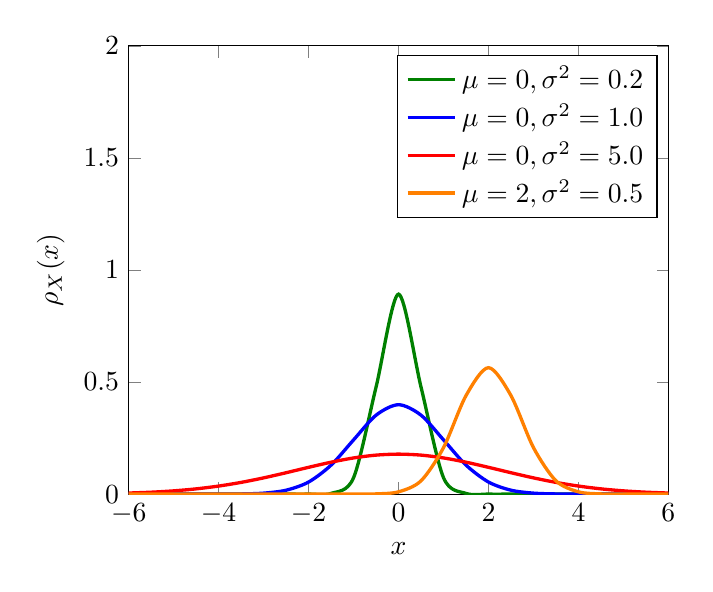
\begin{tikzpicture}[
                declare function={ normal(\x,\mu,\sigmasq) = 1/(sqrt(2*pi*\sigmasq)) * exp(-((\x - \mu)^2) / (2*\sigmasq)); }
            ]
            \begin{axis}[
                xlabel={$x$},
                ylabel={$\rho_X(x)$},
                domain=-6:6,
                ymin=0, ymax=2,
                xmin=-6, xmax=6
            ]

                \addplot [very thick, smooth, Green] {normal(x,0, 0.2)}; \addlegendentry{$\mu = 0, \sigma^2 = 0.2$}
                \addplot [very thick, smooth, blue] {normal(x,0, 1.0)}; \addlegendentry{$\mu = 0, \sigma^2 = 1.0$}
                \addplot [very thick, smooth, red] {normal(x,0, 5.0)}; \addlegendentry{$\mu = 0, \sigma^2 = 5.0$}
                \addplot [very thick, smooth, orange] {normal(x, 2, 0.5)}; \addlegendentry{$\mu = 2, \sigma^2 = 0.5$}
            \end{axis}
            \end{tikzpicture}
        }

        \caption{Funzioni di densità di probabilità di quattro distribuzioni normali.}
    \end{figure}

    Il ruolo centrale nella probabilità e nella statistica della distribuzione normale deriva non solo dalla sua eleganza matematica, ma anche dal fatto che molti fenomeni naturali e sociali, se osservati nel loro comportamento complessivo, tendono ad assumere una forma che ricorda la curva a campana tipica della normale. La distribuzione normale ricopre un ruolo fondamentale in numerosi ambiti:
    \begin{itemize}
        \item \textit{Statistica inferenziale}: molte tecniche di stima e verifica di ipotesi assumono che i dati (o certe trasformazioni degli stessi) seguano una distribuzione normale.

        \item \textit{Fisica e scienze naturali}: errori di misura, fluttuazioni termiche e rumore naturale spesso presentano una componente casuale che può essere modellata come normale.

        \item \textit{Finanza ed economia}: anche se la realtà può essere più complessa, numerosi modelli iniziano assumendo che i rendimenti o le variazioni di certe grandezze abbiano distribuzioni vicine alla normale.

        \item \textit{Psicologia e scienze sociali}: molte variabili aggregate, come punteggi medi o comportamenti collettivi, tendono a distribuirsi in modo approssimativamente normale.
    \end{itemize}

    Un'importante giustificazione teorica all'uso estensivo della distribuzione normale deriva dal \textit{teorema del limite centrale}. Senza entrare nei dettagli, questo risultato afferma in termini molto generali che la somma di molte piccole cause indipendenti tende a produrre una variabile casuale con comportamento vicino a quello della normale. Questo spiega perché la curva a campana ricorre così frequentemente in natura e nelle applicazioni. Torneremo su questo teorema fondamentale nel capitolo successivo.

    \begin{framedprop}{}
        Data una v.a. $X \sim \mathcal{N}(\mu, \sigma^2)$ si ha che:
        \begin{itemize}
            \item $\displaystyle F_X(x) = \frac{1}{2} + \frac{1}{\sqrt{\pi}} \int_{0}^{\frac{x-\mu}{\sigma \sqrt{2}}} e^{-t^2} \diff t$
            \item $\Exp[X] = \mu$
            \item $\mathrm{Var}(X) = \sigma^2$
        \end{itemize}
    \end{framedprop}

    \begin{proof}
        Omessa.
    \end{proof}

    \chapter{Teoremi Limite}

    \section{Limiti superiori di probabilità}

    \subsection{Disuguaglianza di Markov}

    La \textbf{disuguaglianza di Markov} è uno dei risultati fondamentali della teoria della probabilità. Fornisce un limite superiore alla probabilità che una variabile aleatoria positiva assuma valori molto grandi rispetto alla sua media. Informalmente, la disuguaglianza afferma che la probabilità che una v.a. $X$ assume valori molto grandi è molto piccola, proporzionalemnte al suo valore atteso. Conseguentemente, se il valore atteso di $X$ è molto piccolo, è estremamente improbabile che $X$ assuma valori lontani da essa.

    \begin{framedthm}{Disuguaglianza di Markov}
        Sia $X$ una v.a. tale che $X \geq 0$. Allora, per ogni $\ell > 0$ vale che:
        \[\Pr[X \geq \ell] \leq \frac{\Exp[X]}{\ell} \qquad \Pr[X > \ell] < \frac{\Exp[X]}{\ell}\]
        \textit{Nota}: $\Exp[X]$ deve assumere un valore finito. 
    \end{framedthm}

    \begin{proof}
        Consideriamo la funzione indicatrice $\1_{X \geq \ell}$. Poiché $X > 0$, si ha che $X \geq \ell \cdot \1_{X \geq \ell}$ e dunque che:
        \[\1_{X \geq \ell} \leq \frac{X}{\ell}\]

        Per monotonia e linearità del valore atteso, otteniamo che:
        \[\Exp[\1_{X \geq \ell}] \leq \Exp \rbk{\frac{\Exp[X]}{\ell}}\]

        Essendo $\1_{X \geq \ell}$ una Bernoulliana di parametro $p = \Pr[X \geq \ell]$, concludiamo immediatamente che:
        \[\Pr[X \geq \ell] \leq \Exp \rbk{\frac{\Exp[X]}{\ell}}\]

        Procedendo analogamente, possiamo dimostrare anche la seconda disegualianza.
    \end{proof}

    Per capire l'importanza della disuguaglianza di Markov, vediamo alcune sue applicazioni. Prima di tutto, osserviamo che sia possibile generalizzare la disuguaglianza ad una qualsiasi funzione di v.a. $f(X) \geq 0$, ottenendo che:
    \[\Pr[f(X) \geq f(\ell)] \leq \frac{\Exp[f(X)]}{f(\ell)}\]

    Inoltre, è possibile sfruttare la disuguaglianza per ottenere anche un limite inferiore sulla probabilità che una v.a. $X$ si trovi in un determinato intervallo:
    \[\begin{split}
        \Pr[a \leq X \leq b] &= \Pr[X \leq b] - \Pr[X > a] \\
        &= 1 - \Pr[X > b] - \Pr[X > a]\\
        &> 1- \frac{\mu}{b} - \frac{\mu}{a} \\
        &= 1- \frac{\mu(a-b)}{ab}
    \end{split}\] 

    dove $\Exp[X] = \mu$, da cui ne segue anche che:
    \[\Pr[X < a \text{ e } X > b] = 1 - \Pr[a \leq X \leq b] < \frac{\mu(a-b)}{ab}\]

    Riprendiamo ad esempio la variabile $X \sim \mathrm{Bin}(36, 0.5)$ della sezione \Cref{standard}, dove avevamo già calcolato $\mu = 18$ e $\sigma = 3$. Otteniamo quindi che la probabilità che il valore assunto dalla v.a. $X$ si trovi entro due deviazioni dalla media è limitata inferiormente da:
    \[\begin{split}
        \Pr[\abs{X - \mu} \leq 2\sigma] &= \Pr[\mu - 2\sigma \leq X \leq \mu + 2\sigma] \\
        &> 1- \frac{\mu(\mu-2\sigma - \mu - 2\sigma)}{(\mu - 2\sigma)(\mu + 2\sigma)} \\
        &= 1- \frac{\mu(\mu - 4\sigma)}{\mu^2-(2\sigma)^2} \\
        &= 1- \frac{18 (18 - 4 \cdot 3)}{18^2 - (2 \cdot 3)^2} \\
        &= 1- \frac{108}{288} \\
        &\approx 0.6
    \end{split} \]
        
    \subsection{Disuguaglianza di Čebyšëv}

    Nella sezione precedente abbiamo visto come possiamo utilizzare la disuguaglianza di Markov per ottenere un limite inferiore sulla probabilità che una v.a. si discosti entro un certo valore dalla sua media. In particolare, abbiamo visto come il limite inferiore ottenuto sia espresso tramite la media stessa. In alcuni casi, tuttavia, potremmo non essere a conoscenza della media della v.a. in analisi, ma solo della sua varianza (magari attraverso una stima o tramite un parametro dato). In tal caso, può essere utilizzata la \textbf{disuguaglianza di Čebyšëv} (pronunciato \textit{Cebi-shòv} in italiano), la quale invece può fornisce un limite inferiore in termini di varianza.

    \begin{framedthm}{Disuguaglianza di Čebyšëv}
        Sia $X$ una v.a. tale che $X \geq 0$. Allora, per ogni $\ell > 0$ vale che:
        \[\Pr[\abs{X-\mu} \geq \ell] \leq \frac{\mathrm{Var}(X)}{\ell^2} \qquad \Pr[\abs{X-\mu} > \ell] < \frac{\mathrm{Var}(X)}{\ell^2}\]
        \textit{Nota}: $\mathrm{Var}(X)$ deve assumere un valore finito. 
    \end{framedthm}

    \begin{proof}
        Sia $Y = \abs{X-\mu}$ e sia $f(z) = z^2$. Poiché $Y \geq 0$, tramite la disuguaglianza di Markov, abbiamo che:
        \[\Pr[f(Y) \geq f(\ell)] \leq \frac{\Exp[Y]}{f(\ell)}\]
        vale a dire che:
        \[\Pr[\abs{X-\mu}^2 \geq \ell^2] \leq \frac{\Exp[\abs{X-\mu}^2]}{\ell^2}\]

        Per positività de valore assoluto, abbiamo che $\abs{X-\mu}^2 = (X-\mu)^2$, per tanto:
        \[\Pr[\abs{X-\mu}^2 \geq \ell^2] \leq \frac{\Exp[(X-\mu)^2]}{\ell^2} = \frac{\mathrm{Var}(X)}{\ell^2}\]

        Infine, per monotonia di $f(z) = z^2$ nell'intervallo $[0, +\infty)$, abbiamo che $\abs{X-\mu}^2 \geq \ell^2$ se e solo se $\abs{X-\mu} \geq \ell$, concludendo che:
        \[\Pr[\abs{X-\mu} \geq \ell] = \Pr[\abs{X-\mu}^2 \geq \ell^2]  \leq \frac{\mathrm{Var}(X)}{\ell^2}\]

        Procedendo analogamente, possiamo dimostrare anche la seconda disegualianza.
    \end{proof}

    Una volta enunciato il teorema, risulta naturale compararlo con la disuguaglianza di Markov nello stesso esempio precedentemente visto. Sia $X$ sempre la v.a. $X \sim \mathrm{Bin}(36, 0.5)$, dove $\mu = 18$ e $\sigma = 3$. Applicando la disuguaglianza di Čebyšëv otteniamo che:
    \[\begin{split}
        \Pr[\abs{X-\mu} \leq 2\sigma] &= 1 - \Pr[\abs{X-\mu} > 2\sigma] \\
        &> 1 - \frac{\mathrm{Var}(X)}{(2\sigma)^2} \\
        &= 1 - \frac{1}{4} \\
        &= \frac{3}{4} \\
        &= 0.75
    \end{split}\]

    Otteniamo quindi un limite inferiore di $0.75$, molto più stretto rispetto al limite inferiore di circa $0.6$ trovato precedentemente. Generalizzando il processo svolto nell'esempio sopra, affermiamo una versione equivalente della disuguaglianza.

    \begin{framedcor}{Disuguaglianza di Čebyšëv (2° versione)}
        Sia $X$ una v.a. tale che $X \geq 0$ e con $\mathrm{Var}(X)$ finita. Allora, per ogni $\ell > 0$ vale che:
        \[\Pr[\abs{X-\mu} \geq k\sigma] \leq \frac{1}{k^2} \qquad \Pr[\abs{X-\mu} > k\sigma] < \frac{1}{k^2}\]
        \textit{Nota}: $\mathrm{Var}(X)$ deve assumere un valore finito. 
    \end{framedcor}

    \begin{proof}
        Omessa poiché analoga all'esempio precedente.
    \end{proof}
    
    \subsection{Disuguaglianza di Chernoff}

    Concludiamo la nostra discussione sulle disuguaglianze fondamentali del calcolo delle probabilità con la \textbf{disuguaglianza di Chernoff}. A differenza delle disuguaglianze di Markov e Čebyšëv, la disuguaglianza di Chernoff fornisce un limite massimo di forma esponenziale. Questa caratteristica rende la disuguaglianza di fondamentale importanza in contesti con una grande mole di dati in analisi o di parametri molto grandi (calcolo asintotico, machine learning, \dots).
    
    \begin{framedthm}{Disuguaglianza di Chernoff}
        Sia $X$ una v.a. tale che $X \geq 0$. Allora, per ogni $\ell,t > 0$ vale che:
        \[\Pr[X \geq \ell] \leq \frac{\Exp[e^{tX}]}{e^{t\ell}} \qquad \Pr[X > \ell] < \frac{\Exp[e^{tX}]}{e^{t\ell}}\]

        \textit{Nota}: $\Exp[e^{tX}]$ deve assumere un valore finito. 
    \end{framedthm}

    \begin{proof}
        Fissiamo $t > 0$. Per monotonia della funzione $f(z) = e^{tz}$, osserviamo che $X \geq \ell$ se e solo se $e^{tX} \geq e^{t\ell}$, per tando vale che:
        \[\Pr[X \geq \ell] = \Pr[e^{tX} \geq e^{t\ell}]\]

        Poiché $f(X) \geq 0$, tramite la disuguaglianza di Markov concludiamo che:
        \[\Pr[X \geq \ell] = \Pr[f(X) \geq e^{t\ell}] \leq \frac{\Exp[f(X)]}{\ell} = \frac{\Exp[e^{tX}]}{\ell}\]

        Procedendo analogamente, possiamo dimostrare anche la seconda disegualianza.
    \end{proof}

    Poiché il limite superiore ottenuto tramite la disuguaglianza di Chernoff dipende dal valore $\Exp[e^{tX}]$, detto \textit{funzione generatrice dei momenti}, risulta evidente che in base al tipo di variabile aleatoria è possibile rendere il limite molto più specifico. Ad esempio, per le v.a. binomiali è possibile ottenere la seguente disuguaglianza, detta \textbf{errore relativo}.  

    \begin{framedprop}{Errore relativo per binomiali}
        Data una v.a. $X \sim \mathrm{Bin}(n,p)$, per ogni $\delta > 0$ si ha che:
        \[\Pr[X \geq (1+\delta) \mu] \leq \rbk{\frac{e^\delta}{(1+\delta)^{1+\delta}}}^\mu\]
        dove $\Exp[X] = \mu$.
    \end{framedprop}

    \begin{proof}
        Dato un $t > 0$ qualsiasi, per la disuguaglianza di Chernoff abbiamo che:
        \[\Pr[X \geq (1+\delta) \mu] \leq \frac{\Exp[e^{tX}]}{e^{t(1+\delta)\mu}}\]

        Siano quindi $X_1, \ldots, X_n \in \mathcal{B}(p)$ le v.a. indipendenti tali che $X = X_1 + \ldots + X_n$. Osserviamo che:
        \[\Exp[e^{tX}] = \Exp[e^{t(X_1+ \ldots + X_n)}] = \Exp[e^{tX_1} \cdot \ldots \cdot e^{tX_n}] = \Exp[e^{tX_1}] \cdot \ldots \cdot \Exp[e^{tX_n}] = \Exp[e^{tX_1}]^n\]

        \textbf{Fatto}: $\Exp[e^{tX_1}] \leq e^{np(e^t-1)}$
        
        \begin{proof}
            Data $f(z) = e^{tz}$, abbiamo che:
            \[\begin{split}
                \Exp[e^{tX_1}] &= e^{t\cdot 0} \Pr[X = 0] + e^{t \cdot 1} \Pr[X = 1] \\
                &= (1-p) + pe^t \\
                &= 1+p(e^t-1)
            \end{split}\]

            Tramite la disuguaglianza nota $e^x \geq x+1$, concludiamo che:
            \[\Exp[e^{tX_1}] = 1+p(e^t-1) \leq e^{p(e^t)-1}\]
        \end{proof}

        Otteniamo quindi che:
        \[\begin{split}
            \Pr[X \geq (1+\delta) \mu] &\leq \frac{\Exp[e^{tX_1}]^n}{e^{t(1+\delta)\mu}} \leq  e^{-t(1+\delta)\mu} e^{\mu(e^t-1)}
        \end{split}\]

        A questo punto, scegliendo $t = \log(\delta + 1)$, otteniamo che:
        \[\begin{split}
            \Pr[X \geq (1+\delta) \mu] &\leq  e^{-\log(\delta+1) (1+\delta)\mu} e^{\mu(e^{\log(\delta+1)}-1)}\\
            &= (\delta+1)^{-(1+\delta)} e^{\mu(\delta+1-1)} \\
            &= \rbk{\frac{e^\delta}{(1+\delta)^{1+\delta}}}^\mu
        \end{split}\]
    \end{proof}

    \section{Legge dei grandi numeri}

    Supponiamo di star giocando a testa o croce con il nostro amico Arnaldo, il quale sceglie il segno \textit{croce} -- dunque a noi spetterà il segno \textit{testa}. Supponiamo ora di effettuare $n$ lanci indipendenti con la stessa moneta non truccata, ossia con probabilità $\frac{1}{2}$ per entrambi gli esiti.
    
    Definiamo quindi una variabile aleatoria $X_i \sim \mathcal{B}(0.5)$ per ogni lancio $i$ che effettuiamo, dove $X_i = 1$ se l'esito è testa.Per buonsenso umano, ci aspettiamo che all'aumentare del numero $n$ di lanci la quantità di esiti testa sarà più o meno alla quantità degli esiti croce. In altre parole, ci aspettiamo che la quantità di teste ottenute sia più o meno uguale alla metà dei lanci totali. Formalmente, stiamo affermando che la \textbf{media campionaria} $\overline{X}_n$ si avvicini al valore atteso $\Exp[X_1] = \ldots = \Exp[X_n] = \frac{1}{2}$, dove:
    \[\overline{X}_n = \frac{X_1 + \ldots + X_n}{n}\]

    La \textbf{legge dei grandi numeri} formalizza questo principio affermando che, con l'aumentare del numero di osservazioni \textit{i.i.d. (indipendenti e identicamente distribuite)} dello stesso tipo, la media dei risultati osservati si avvicina alla media teorica del fenomeno. Questo risultato è alla base del metodo scientifico basato sulla misurazione ripetuta e costituisce uno dei pilastri dell'inferenza statistica.
    
    La legge dei grandi numeri riveste un ruolo centrale nella teoria della probabilità e nella statistica perché fornisce una giustificazione matematica al processo di stima dei parametri attraverso osservazioni ripetute. In molte situazioni reali non è possibile conoscere esattamente il valore medio di un fenomeno poiché descritto da variabili aleatorie troppo complesse; tuttavia, raccogliendo un numero sufficientemente ampio di dati, possiamo ottenere stime affidabili.
    
    In particolare, la legge si distingue in due formulazioni dette \textbf{legge debole} e \textbf{legge forte}. La legge debole afferma che per ogni $\varepsilon > 0$ è \textit{asintoticamente quasi certo} che la distanza tra la media campionaria e il valore atteso sia minore di $\varepsilon$, mentre la legge forte afferma che è \textit{quasi certo} che asintoticamente la media campionaria coincida con il valore atteso (si noti il cambio di prospettiva tra le due formulazioni).

    \begin{framedthm}{Legge debole dei grandi numeri}
        Data una successione di v.a. $X_1, \ldots, X_n$ i.i.d., per ogni $\varepsilon > 0$ vale che:
        \[\lim_{n \to +\infty} \Pr[\abs{\overline{X}_n - \mu} < \varepsilon] = 1\]
        dove $\mu = \Exp[X_i]$ per ogni $i \in [n]$. 
    \end{framedthm}

    \begin{proof}
        Essendo $X_1, \ldots, X_n$ i.i.d., si ha che:
        \[\Exp[\overline{X}_n] = \Exp \sbk{\frac{X_1 + \ldots + X_n}{n}} = \frac{1}{n} \sum_{i = 1}^n \Exp[X_i] = \frac{n\mu}{n} = \mu\]
        
        Similmente, abbiamo che:
        \[\mathrm{Var}(\overline{X}_n) = \mathrm{Var}\rbk{\frac{X_1 + \ldots + X_n}{n}} = \frac{1}{n^2} \sum_{i = 1}^n \mathrm{Var}(X_i) = \frac{\mathrm{Var}(X_1)}{n}\]

        Per tanto, tramite la disugualianza di Čebyšëv abbiamo che:
        \[\Pr[\abs{\overline{X}_n - \mu} \geq \varepsilon] \leq \frac{\mathrm{Var}(\overline{X}_n)}{\varepsilon^2} = \frac{\mathrm{Var}(X_1)}{n\varepsilon^2}\]

        A questo punto, ricordando che $\Pr$ è una funzione non-negativa, per il teorema dei carabinieri concludiamo che:
        \[\lim_{n \to +\infty} 0 \leq \lim_{n \to +\infty} \Pr[\abs{\overline{X}_n - \mu} \geq \varepsilon] \leq \lim_{n \to +\infty} \frac{\mathrm{Var}(X_1)}{n\varepsilon^2} = \lim_{n \to +\infty} 0 \]

        vale a dire che:
        \[\lim_{n \to +\infty} \Pr[\abs{\overline{X}_n - \mu} \geq \varepsilon] = 0\]
    \end{proof}

    \begin{framedthm}{Legge forte dei grandi numeri}
        Data una successione di v.a. $X_1, \ldots, X_n$ i.i.d., per ogni $\varepsilon > 0$ vale che:
        \[\Pr\sbk{\lim_{n \to +\infty} \overline{X}_n = \mu} = 1\]
        dove $\mu = \Exp[X_i]$ per ogni $i \in [n]$. 
    \end{framedthm}

    \begin{proof}
        Omessa per complessità.
    \end{proof}

    \section{Teorema del limite centrale}

    Nella sezione precedente abbiamo visto come la legge dei grandi numeri stabilisca che, all'aumentare del numero di osservazioni i.i.d. effettuate, la media campionaria tenda a coincidere con il valore atteso, fornendo una sorta di \curlyquotes{ponte} tra l'evidenza empirica e il formalismo matematico. Procedendo sulla stessa idea, il \textbf{teorema del limite centrale} rafforza questo ponte costituendo uno dei risultati fondamentali della teoria della probabilità e il fondamento dell'inferenza statistica moderna.
    
    Il teorema afferma che, sempre all'aumentare del numero di osservazioni i.i.d. effettuate, la media campionaria e la somma campionaria tendano a seguire una particolare legge di distribuzione, ossia la \textit{distribuzione normale}, indipendentemente dai parametri che descrivono le distribuzioni delle osservazioni. In particolare, la funzione di ripartizione della standardizzata $S_n^*$ della variabile $S_n = X_1 + \ldots + X_n$ con $X_1, \ldots, X_n$ i.i.d., tende alla funzione $\Phi(x)$, definita come la funzione di ripartizione di $\mathcal{N}(0,1)$:
    \[\Phi(x) = \frac{1}{2} + \frac{1}{\sqrt{\pi}} \int_{0}^{\frac{x}{\sqrt{2}}} e^{-t^2} \diff t \] 
    
    Questo risultato fornisce il collegamento tra fenomeni aleatori di natura potenzialmente complessa e l'ampio utilizzo del modello normale nella pratica statistica, mostrando come un vasto insieme insieme di piccole incertezze diano vita a qualcosa di straordinariamente regolare.

    \begin{framedthm}{Teorema del limite centrale}
        Si consideri una successione di v.a. $X_1, \ldots, X_n$ i.i.d. con $\Exp[X_i] = \mu$ e $\mathrm{Var}(X_i) = \sigma^2$. Data la standardizzata $S^*_n$ di $S_n = X_1 + \ldots + X_n$, ossia:
        \[S^*_n = \frac{S_n - n\mu}{\sqrt{n \sigma^2}}\]
        per $n \to +\infty$ la funzione di ripartizione $F_{\overline{X}^*_n}(x)$ tende alla funzione di ripartizione $\Phi$ di $\mathcal{N}(0,1)$. 
        \[\lim_{n \to +\infty} F_{S^*_n}(x) = \Phi(x)\]
    \end{framedthm}

    \begin{proof}
        Omessa per complessità.
    \end{proof}

    L'enunciato riportato è formulato in termini della somma campionaria $S_n$, ma in alcuni libri di testo viene anche formulato in termini della media campionaria $\overline{X}_n$. In tali versioni, data la standardizzata $\overline{X}^*_n$ di $\overline{X}_n$, ossia:
    \[\overline{X}^*_n = \frac{\overline{X}_n - \mu}{\sigma / \sqrt{n}}\]
    per $n \to +\infty$ la funzione di ripartizione $F_{\overline{X}^*_n}(x)$ tende alla funzione di ripartizione $\Phi$ di $\mathcal{N}(0,1)$. 
    \[\lim_{n \to +\infty} F_{\overline{X}^*_n}(x) = \Phi(x)\]

    È possibile ottenere questa formulazione tramite la media campionaria semplicemente applicando la formulazione tramite la somma sulle variabili $Y_1, \ldots, Y_n$ tali che $Y_i = X_i / n$ per ogni $i \in [n]$ (da cui deriva che $\Exp[Y_i] = \Exp[X_i] / n$ e $\mathrm{Var}(Y_i) = \mathrm{Var}(X_i) / n^2$).

    Osserviamo come il teorema del limite centrale abbia una speciale applicazione nel caso delle distribuzioni binomiali. Poiché ogni v.a. binomiale $X \sim \mathrm{Bin}(n,p)$ è per definizione uguale alla somma di $n$ v.a. i.i.d. di Bernoulli $X_1, \ldots, X_n \sim \mathcal{B}(p)$, il teorema del limite centrale ci dice che all'aumentare di $n$ l'intera distribuzione tenderà ad assumere la forma di una curva a campana. Questa particolare proprietà fù inizialmente osservata da De Moivre, ben prima della scoperta del teorema del limite centrale.

    \begin{framedcor}{Teorema di De Moivre}
        Data una v.a. $X \sim \mathrm{Bin}(n,p)$ e la sua standardizzata $Z$, si ha che:
        \[\lim_{n \to +\infty} F_Z(x) = \Phi(x)\]
        dove $\Phi$ è funzione di ripartizione di $\mathcal{N}(0,1)$. 
    \end{framedcor}
    
    \begin{figure}[H]
        \centering
        \includegraphics[scale=0.6]{images/CLTBinomConvergence.pdf}
        \caption{Lo sviluppo di una serie binomiale di valori casuali e la sua convergenza alla distribuzione normale.}
    \end{figure}

    Proviamo ora a ragionare sulle altre distribuzioni discusse, discutendo se esse siano influenzate dal teorema del limite centrale. Nel \Cref{disc_var} abbiamo visto come la distribuzione ipergeometrica sia descrivibile come somma di un tipo molto specifico di variabili di Bernoulli, dando vita quindi ad un ragionamento simile al caso binomiale per quanto riguarda la sua forma a campana. Similmente, abbiamo visto come la distribuzione di Pascal sia definita come una somma di geometriche i.i.d., coincidendo ancora una volta il teorema del limite centrale. Per quanto riguarda la distribuzione di Poisson, invece, abbiamo visto come essa coincida ad un limite particolare della distribuzione binomiale, dunque essa tenderà chiaramente ad una forma a campana. 

    Rimane quindi da considerare solo la distribuzione geometrica (e quella esponenziale essendo la sua versione continua). Sebbene il suo grafico ricordi molto la \curlyquotes{parte destra} della curva a campana, ciò risulta essere solo una coincidenza: non è una diretta influenza del teorema del limite centrale (si pensi al fatto che anche la distribuzione esponenziale è definita da un esponenziale negativo, dunque assumerà una forma simile alla curva di Gauss).

    Osserviamo inoltre che il teorema del limite centrale può essere utilizzato per applicare le cosidette \textbf{approssimazioni normali}. L'idea è quella di approssimare la funzione di ripartizione di una v.a. tramite il fatto che l'errore tra le funzioni di ripartizione della sua standardizzata e della Gaussiana normale tenda a 0.
    
    \begin{framedprop}{Approssimazione normale}
        Si consideri una successione di v.a. $X_1, \ldots, X_n$ i.i.d. con $\Exp[X_i] = \mu$ e $\mathrm{Var}(X_i) = \sigma^2$. Data v.a. $S_n = X_1 + \ldots + X_n$, si ha che:
        \[F_{S_n}(x) \approx \Phi\rbk{\frac{x-n \mu}{\sqrt{n \sigma^2}}}\]
        dove $\Phi$ è la funzione di ripartizione di $\mathcal{N}(0,1)$.
    \end{framedprop}

    \begin{proof}
        Sia $S^*_n$ la standardizzata di $S_n$ e sia $E_n$ la funzione di errore tra le due distribuzioni, ossia:
        \[E_n(x) = F_{S^*_n}(x)-\Phi(x)\]

        Sia inoltre $x_n$ definito come:
        \[x_n = \frac{x - n\mu}{\sqrt{n \sigma^2}}\]

        Tramite semplice manipolazione algebrica, abbiamo che:
        \[\begin{split}
            F_{S_n}(x) &= \Pr[S_n \leq x] \\
            &= \Pr\sbk{\frac{S_n - n\mu}{\sqrt{n \sigma^2}} \leq \frac{x - n\mu}{\sqrt{n \sigma^2}}} \\
            &= F_{S_n^*}(x_n) \\
            &= \Phi(x_n) + E_n(x_n)
        \end{split}\]

        Per tanto, vale che:
        \[\abs{F_{S_n}(x) - \Phi(x_n)} = \abs{E_n(x_n)} \leq \sup_{x' \in \R} \abs{E_n(x')}\]

        Per il teorema del limite centrale, sappiamo che $\sup_{x' \in \R} \abs{E_n(x')} \to 0$ quando $n \to +\infty$, rendendo l'errore trascurabile.
    \end{proof}

    Come conseguenza dell'approssimazione normale, possiamo ottenere una \curlyquotes{versione approssimata} della legge dei grandi numeri. Si consideri una successione di v.a. $X_1, \ldots, X_n$ i.i.d. con $\Exp[X_i] = \mu$ e $\mathrm{Var}(X_i) = \sigma^2$. Data v.a. $S_n = X_1 + \ldots + X_n$, osserviamo che:
    \[\overline{X}_n - \mu = \frac{S_n - n\mu}{n}\]

    da cui deriviamo che:
    \[\begin{split}
        \Pr[\abs{\overline{X}_n - \mu} \leq \varepsilon] &= \Pr[ -\varepsilon \leq \frac{S_n-n\mu}{n} \leq \varepsilon] \\
        &= \Pr\sbk{- \sqrt{\frac{n}{\sigma^2}} \varepsilon \leq \frac{S_n-n\mu}{\sqrt{n \sigma^2}} \leq \sqrt{\frac{n}{\sigma^2}} \varepsilon} \\
        &= F_{S_n^*}\rbk{\sqrt{\frac{n}{\sigma^2}}} + \Pr\sbk{\frac{S_n-n\mu}{\sqrt{n \sigma^2}} = -\sqrt{\frac{n}{\sigma^2}} \varepsilon} - F_{S_n^*}\rbk{-\sqrt{\frac{n}{\sigma^2}}} \\
        &\approx \Phi\rbk{\sqrt{\frac{n}{\sigma^2}}} - \Phi\rbk{-\sqrt{\frac{n}{\sigma^2}}} \\
        & = 2\Phi\rbk{\sqrt{\frac{n}{\sigma^2}}} - 1
    \end{split}\]

    dove $S_n^*$ è la standardizzata di $S_n$. Per $n \to +\infty$, abbiamo che:
    \[\lim_{n \to +\infty} \Phi\rbk{\sqrt{\frac{n}{\sigma^2}}} = \lim_{n \to +\infty} \frac{1}{2} + \frac{1}{\sqrt{\pi}} \int_{0}^{\sqrt{\frac{2n}{\sigma^2}}} e^{-t^2} \diff t = 2\]

    concludendo quindi la stessa tesi della legge dei grandi numeri:
    \[\lim_{n \to +\infty} \Pr[\abs{\overline{X}_n - \mu} \leq \varepsilon] = 2 - 1 = 1\]

\end{document}

